%\documentclass[fontsize=13pt,a4paper,oneside, DIV=calc, chapterprefix=true]{scrbook} % twoside for draft
\documentclass[fontsize=13pt,a4paper]{report}  
 
%\documentclass[13pt,a4paper,oneside]{book} % twoside for draf

%\usepackage{babel}
\usepackage[utf8,nocaptions]{vietnam}
\usepackage[vietnamese]{babel}
%\usepackage{times}
%\usepackage{graphicx}

\usepackage{husthesis-en}
\usepackage{enumitem}

 
\usepackage{tipa}
\usepackage{amssymb}
\usepackage{graphicx}
\usepackage{subcaption}
\usepackage{booktabs}
\usepackage{mathptmx}	% same Time New Roma
\usepackage{amsmath}
\usepackage{amsfonts}
%\usepackage{sty/ipa}
%\renewcommand{\rmdefault}{phv} % Arial
%\renewcommand{\sfdefault}{phv} % Arial
%\renewcommand\thesection{\arabic{section}}

\usepackage{array}
\newcolumntype{P}[1]{>{\centering\arraybackslash}p{#1}}
\newcolumntype{M}[1]{>{\centering\arraybackslash}m{#1}}
\usepackage{fancyhdr}
\usepackage{multirow}
\usepackage[linesnumbered,ruled,vlined]{algorithm2e}
\usepackage{float}
\usepackage{placeins}
\usepackage{listings}
\usepackage{hyperref}
\hypersetup{
    colorlinks=true,
    linkcolor=blue,
    filecolor=magenta,      
    urlcolor=cyan,
}


%\crname{Tiểu luận khoa học}
\ctname{ỨNG DỤNG \\ CÁC MÔ HÌNH QUY HOẠCH TUYẾN TÍNH \\ CHO CÁC LOẠI BÀI TOÁN KNAPSACK}
\cstuname{
Nguyễn Hoàng Đạt - 24001989 \\
Nguyễn Hải Anh - 24001968 \\
Lê Sỹ Thức - 25000312 \\
}

\csMajor{Khoa học máy tính và thông tin}
\cttime{2026}

\thesislayout

\counterwithout{section}{chapter} 
 
\begin{document}

\coverpage

\secondcoverpage

%\frontmatter


% \begin{declaration}
% We, <fullnames of students>, hereby declare that this report titled "<report title>" is our own work. It reflects our understanding and analysis of the documents assigned to us. 

% We confirm that:
% \begin{itemize}
%     \item All sources used are properly cited and acknowledged.
%     \item This report has not been submitted for any other course or purpose.
%     \item While the report may include corrections made with the assistance of ChatGPT or similar tools, it was not generated by such tools.
%     \item We understand that failure to comply with these principles will result in a score of zero for this report.
% \end{itemize}
% \end{declaration}

%\begin{acknowledgments}
 
%\end{acknowledgments}

\begin{abstract}
Ra đời vào năm 1947 và được xem là một trong những thuật toán có ảnh hưởng sâu rộng nhất của thế kỷ XX, thuật toán đơn hình (simplex method) đóng vai trò nền tảng trong lĩnh vực quy hoạch tuyến tính và tối ưu hóa. Sự phát triển của các biến thể như thuật toán đơn hình hai pha và thuật toán đơn hình đối ngẫu đã mở rộng đáng kể khả năng ứng dụng của phương pháp này trong nhiều bài toán tối ưu thực tiễn thuộc khoa học, kỹ thuật và công nghiệp.

Bài toán cái túi (Knapsack Problem) là một trong những bài toán tối ưu tổ hợp kinh điển của khoa học máy tính, với nhiều ứng dụng trong phân bổ tài nguyên, quản lý danh mục đầu tư, lập lịch sản xuất và hỗ trợ ra quyết định. Trong báo cáo này, chúng tôi khảo sát ba biến thể quan trọng của bài toán knapsack gồm fractional knapsack, unbounded knapsack và 0/1 knapsack dưới góc nhìn của quy hoạch tuyến tính và quy hoạch nguyên. Trên cơ sở đó, báo cáo trình bày việc áp dụng các phương pháp đơn hình, bao gồm đơn hình nguyên thủy, đơn hình hai pha và đơn hình đối ngẫu, để giải các mô hình tương ứng.

Ngoài việc phân tích mô hình toán học và cơ chế hoạt động của các thuật toán, báo cáo còn đánh giá hiệu quả thực nghiệm của các phương pháp dựa trên quy hoạch tuyến tính, đồng thời so sánh chúng với các chiến lược thiết kế thuật toán kinh điển như vét cạn, quay lui, nhánh-cận, tham lam và quy hoạch động. Qua đó, báo cáo làm rõ ưu điểm, hạn chế cũng như tiềm năng ứng dụng của các phương pháp đơn hình trong việc giải các bài toán knapsack và các bài toán tối ưu tổ hợp mở rộng.
\end{abstract}
 
% Danh sách từ viết tắt
% \nomenclature{CIS}{Computer and Information Science}
\printnomenclature

\tableofcontents
% \listoftables
% \listoffigures
\vfil\null\endtitlepage
%\listofalgorithms

%\mainmatter

\fancyhead{}  % Clears all page headers and footers
%\rhead{\thepage}  % Sets the right side header to show the page number
%\lhead{}  % Clears the left side page header
%\fancyfoot[positions]{footer}
\renewcommand{\footrulewidth}{0.4pt}

\pagestyle{fancy}  % Finally, use the "fancy" page style to implement the FancyHdr headers
%


% ============================================================================
% SECTION 1: GIỚI THIỆU
% ============================================================================
\section{Giới thiệu}
\label{sec:intro}

Bài toán cái túi (Knapsack Problem) là một trong những bài toán tối ưu tổ hợp nền tảng trong khoa học máy tính và vận trù học. Bài toán được phát biểu đơn giản: cho một tập các vật phẩm, mỗi vật phẩm có trọng lượng và giá trị riêng, hãy chọn một tập con các vật phẩm sao cho tổng giá trị là lớn nhất mà tổng trọng lượng không vượt quá sức chứa của cái túi.

Mặc dù phát biểu đơn giản, bài toán Knapsack thuộc lớp NP-hard~\cite{karp1972reducibility}, nghĩa là chưa tồn tại thuật toán nào giải được mọi trường hợp trong thời gian đa thức (trừ khi P = NP). Điều này khiến bài toán trở thành đối tượng nghiên cứu quan trọng về mặt lý thuyết lẫn thực tiễn.

\textbf{Ứng dụng thực tiễn.} Bài toán Knapsack xuất hiện trong nhiều lĩnh vực:
\begin{itemize}[noitemsep]
    \item \textit{Phân bổ tài nguyên}: phân bổ ngân sách, lập lịch dự án với tài nguyên giới hạn.
    \item \textit{Quản lý danh mục đầu tư}: chọn tổ hợp tài sản tối ưu với vốn giới hạn.
    \item \textit{Logistics}: xếp hàng vào container, xe tải với trọng tải giới hạn.
    \item \textit{Mật mã học}: hệ mã Merkle--Hellman dựa trên bài toán Knapsack.
\end{itemize}

\textbf{Mục tiêu đề tài.} Báo cáo này tiếp cận bài toán Knapsack từ góc độ \textit{quy hoạch tuyến tính} (LP) và \textit{quy hoạch nguyên} (IP). Cụ thể, chúng tôi:
\begin{enumerate}[noitemsep]
    \item Trình bày ba biến thể chính: 0/1, Unbounded và Fractional Knapsack.
    \item Phân tích các chiến lược giải cơ bản: vét cạn, quay lui, nhánh cận, tham lam, quy hoạch động.
    \item Xây dựng mô hình LP/IP và áp dụng các thuật toán Simplex, lời giải đối ngẫu, lát cắt Gomory.
    \item Thực nghiệm so sánh hiệu năng trên bộ dữ liệu benchmark với các mức độ phức tạp khác nhau.
\end{enumerate}


% ============================================================================
% SECTION 2: CÁC LOẠI BÀI TOÁN KNAPSACK
% ============================================================================
\section{Một số loại bài toán Knapsack}
\label{sec:knapsack_intro}

Trong phần này, chúng tôi trình bày ba biến thể phổ biến nhất của bài toán Knapsack~\cite{kellerer2004knapsack}. Sự khác biệt cốt lõi giữa chúng nằm ở \textbf{miền giá trị của biến quyết định} $x_i$: nhị phân (0/1), nguyên không âm (Unbounded), hoặc liên tục trên $[0,1]$ (Fractional).

Xét bài toán tổng quát với $n$ vật phẩm, vật phẩm thứ $i$ có trọng lượng $w_i > 0$, giá trị $v_i > 0$, và cái túi có sức chứa $W > 0$.


% --- 2.1: 0/1 KNAPSACK ---
\subsection{0/1 Knapsack}

Trong bài toán 0/1 Knapsack, mỗi vật phẩm chỉ có thể được \textbf{chọn hoặc không chọn} (không chia nhỏ, không lặp lại). Biến quyết định $x_i \in \{0, 1\}$.

\textbf{Mô hình toán học:}
\begin{align}
    \text{Maximize} \quad & \sum_{i=1}^{n} v_i \cdot x_i \label{eq:01obj} \\
    \text{subject to} \quad & \sum_{i=1}^{n} w_i \cdot x_i \leq W \label{eq:01cap} \\
    & x_i \in \{0, 1\}, \quad \forall i = 1, \ldots, n \label{eq:01bin}
\end{align}

Đây là một bài toán \textbf{quy hoạch nguyên nhị phân} (Binary Integer Programming). Ràng buộc~(\ref{eq:01bin}) khiến bài toán thuộc lớp NP-hard~\cite{karp1972reducibility}, do không gian tìm kiếm có kích thước $2^n$.

\textbf{Ví dụ.} Cho 4 vật phẩm và sức chứa $W = 5$:

\begin{table}[H]
\centering
\begin{tabular}{c|cccc}
\toprule
Vật phẩm $i$ & A & B & C & D \\
\midrule
Trọng lượng $w_i$ & 2 & 1 & 3 & 2 \\
Giá trị $v_i$ & 12 & 10 & 20 & 15 \\
Mật độ $v_i/w_i$ & 6.0 & 10.0 & 6.67 & 7.5 \\
\bottomrule
\end{tabular}
\caption{Dữ liệu ví dụ cho bài toán Knapsack}
\label{tab:example_items}
\end{table}

Nghiệm tối ưu: chọn $\{A, B, D\}$ với tổng trọng lượng $2+1+2=5 = W$, tổng giá trị $12+10+15 = 37$.


% --- 2.2: UNBOUNDED KNAPSACK ---
\subsection{Unbounded Knapsack}

Trong bài toán Unbounded Knapsack, mỗi vật phẩm có thể được chọn \textbf{không giới hạn số lần}. Biến quyết định $x_i \in \mathbb{Z}_{\geq 0}$ (số nguyên không âm).

\textbf{Mô hình toán học:}
\begin{align}
    \text{Maximize} \quad & \sum_{i=1}^{n} v_i \cdot x_i \label{eq:ubobj} \\
    \text{subject to} \quad & \sum_{i=1}^{n} w_i \cdot x_i \leq W \label{eq:ubcap} \\
    & x_i \in \mathbb{Z}_{\geq 0}, \quad \forall i = 1, \ldots, n \label{eq:ubint}
\end{align}

So với 0/1 Knapsack, miền biến mở rộng từ $\{0,1\}$ sang $\mathbb{Z}_{\geq 0}$, cho phép khai thác triệt để các vật phẩm có mật độ giá trị cao. Bài toán vẫn thuộc lớp NP-hard, tuy nhiên có thể giải bằng quy hoạch động với độ phức tạp giả đa thức $O(nW)$.

\textbf{Ví dụ.} Với dữ liệu Bảng~\ref{tab:example_items} và $W=5$: vật phẩm B có mật độ cao nhất ($v/w = 10$), chọn B $\times 5$ lần cho trọng lượng $1 \times 5 = 5$ và giá trị $10 \times 5 = 50$.


% --- 2.3: FRACTIONAL KNAPSACK ---
\subsection{Fractional Knapsack}

Trong bài toán Fractional Knapsack, mỗi vật phẩm có thể được chọn \textbf{một phần} (phân số từ 0 đến 1). Biến quyết định $x_i \in [0, 1]$.

\textbf{Mô hình toán học:}
\begin{align}
    \text{Maximize} \quad & \sum_{i=1}^{n} v_i \cdot x_i \label{eq:frobj} \\
    \text{subject to} \quad & \sum_{i=1}^{n} w_i \cdot x_i \leq W \label{eq:frcap} \\
    & 0 \leq x_i \leq 1, \quad \forall i = 1, \ldots, n \label{eq:frfrac}
\end{align}

Đây chính là bài toán \textbf{quy hoạch tuyến tính} (LP). Khác biệt quan trọng: miền biến liên tục $[0,1]$ thay vì rời rạc, do đó bài toán giải được trong \textbf{thời gian đa thức} bằng chiến lược tham lam hoặc thuật toán Simplex~\cite{dantzig1957discrete}.

Fractional Knapsack đóng vai trò quan trọng như \textbf{LP relaxation} của bài toán 0/1 Knapsack: nới lỏng ràng buộc $x_i \in \{0,1\}$ thành $x_i \in [0,1]$. Nghiệm tối ưu của LP relaxation luôn $\geq$ nghiệm tối ưu 0/1, tạo cận trên cho thuật toán Nhánh cận.

\textbf{Ví dụ.} Với dữ liệu Bảng~\ref{tab:example_items} và $W=5$: sắp xếp theo mật độ giảm dần $B(10) > D(7.5) > C(6.67) > A(6)$, chọn lần lượt:
\begin{itemize}[noitemsep]
    \item B toàn bộ ($x_B=1$): trọng lượng $1$, còn lại $4$.
    \item D toàn bộ ($x_D=1$): trọng lượng $2$, còn lại $2$.
    \item C một phần ($x_C=2/3$): trọng lượng $3 \times 2/3 = 2$, còn lại $0$.
\end{itemize}
Tổng giá trị: $10 + 15 + 20 \times 2/3 = 38.33$. Lưu ý giá trị này cao hơn nghiệm 0/1 tối ưu ($37$).


\textbf{So sánh tổng hợp.} Bảng~\ref{tab:compare_variants} tóm tắt sự khác biệt giữa ba biến thể.

\begin{table}[H]
\centering
\begin{tabular}{l|ccc}
\toprule
\textbf{Đặc điểm} & \textbf{0/1} & \textbf{Unbounded} & \textbf{Fractional} \\
\midrule
Miền biến $x_i$ & $\{0, 1\}$ & $\mathbb{Z}_{\geq 0}$ & $[0, 1]$ \\
Loại mô hình & ILP & IP & LP \\
Độ phức tạp & NP-hard & NP-hard & $O(n \log n)$ \\
Nghiệm ví dụ & 37 & 50 & 38.33 \\
\bottomrule
\end{tabular}
\caption{So sánh ba biến thể bài toán Knapsack}
\label{tab:compare_variants}
\end{table}


% ============================================================================
% SECTION 3: CÁC CHIẾN LƯỢC CƠ BẢN
% ============================================================================
\section{Các chiến lược cơ bản}
\label{sec:basic_strategies}

Phần này trình bày các chiến lược giải cơ bản cho bài toán Knapsack. Với mỗi chiến lược, chúng tôi phân tích: (1) ý tưởng, (2) mã giả, (3) độ phức tạp thời gian và bộ nhớ, (4) tính chính xác của nghiệm.


% --- 3.1: VÉT CẠN, QUAY LUI ---
\subsection{Vét cạn và Quay lui}

\subsubsection*{Vét cạn (Brute Force)}

\textbf{Ý tưởng.} Liệt kê tất cả $2^n$ tập con của $n$ vật phẩm, kiểm tra tính khả thi (tổng trọng lượng $\leq W$), và chọn tập con có giá trị lớn nhất.

Đây là phương pháp đơn giản nhất, luôn tìm được nghiệm tối ưu, nhưng có độ phức tạp theo hàm mũ khiến nó chỉ khả thi với $n$ rất nhỏ.

\begin{itemize}[noitemsep]
    \item \textbf{Độ phức tạp thời gian:} $O(2^n)$ -- duyệt tất cả tập con.
    \item \textbf{Độ phức tạp bộ nhớ:} $O(n)$ -- lưu tập con hiện tại.
    \item \textbf{Tính chính xác:} Luôn cho nghiệm \textbf{tối ưu}.
\end{itemize}

\subsubsection*{Quay lui (Backtracking)}

\textbf{Ý tưởng.} Cải tiến vét cạn bằng cách xây dựng nghiệm dần dần trên cây nhị phân (mỗi nút ứng với quyết định chọn/không chọn vật phẩm $i$), kết hợp \textbf{cắt tỉa} (pruning) để loại bỏ sớm các nhánh không triển vọng.

Chiến lược cắt tỉa: tại mức $i$, nếu giá trị hiện tại cộng tổng giá trị của tất cả vật phẩm còn lại vẫn không vượt qua nghiệm tốt nhất đã biết, ta bỏ qua nhánh này.

\begin{algorithm}[H]
\caption{Quay lui cho 0/1 Knapsack}
\label{alg:backtracking}
\KwIn{Vật phẩm $(w_i, v_i)_{i=1}^{n}$, sức chứa $W$}
\KwOut{Giá trị tối ưu $V^*$, tập chọn $S^*$}
$V^* \leftarrow 0;\; S^* \leftarrow \emptyset$\;
Tính trước: $\text{suffix}[i] = \sum_{j=i}^{n} v_j$ \tcp*{tổng giá trị từ $i$ đến $n$}
\SetKwFunction{FBT}{Backtrack}
\SetKwProg{Fn}{Function}{:}{}
\Fn{\FBT{$i,\; w,\; v,\; S$}}{
    \If{$v > V^*$}{
        $V^* \leftarrow v;\; S^* \leftarrow S$\;
    }
    \If{$i > n$}{\Return}
    \If(\tcp*[f]{Cắt tỉa}){$v + \text{suffix}[i] \leq V^*$}{\Return}
    \If(\tcp*[f]{Chọn vật phẩm $i$}){$w + w_i \leq W$}{
        \FBT{$i+1,\; w+w_i,\; v+v_i,\; S \cup \{i\}$}\;
    }
    \FBT{$i+1,\; w,\; v,\; S$} \tcp*{Không chọn vật phẩm $i$}
}
\FBT{$1,\; 0,\; 0,\; \emptyset$}\;
\Return $V^*,\; S^*$\;
\end{algorithm}

\begin{itemize}[noitemsep]
    \item \textbf{Độ phức tạp thời gian:} $O(2^n)$ trường hợp xấu nhất, nhưng cắt tỉa giúp giảm đáng kể trong thực tế.
    \item \textbf{Độ phức tạp bộ nhớ:} $O(n)$ -- ngăn xếp đệ quy sâu tối đa $n$.
    \item \textbf{Tính chính xác:} Luôn cho nghiệm \textbf{tối ưu} (duyệt đủ không gian nghiệm).
    \item \textbf{Phù hợp:} $n \leq 25$.
\end{itemize}


% --- 3.2: NHÁNH CẬN ---
\subsection{Nhánh cận (Branch and Bound)}

\textbf{Ý tưởng.} Nhánh cận~\cite{land1960automatic} cải tiến quay lui bằng cách sử dụng \textbf{cận trên} (upper bound) chặt hơn để cắt nhánh. Thay vì dùng tổng giá trị còn lại (lỏng), ta tính cận trên từ \textbf{LP relaxation} (Fractional Knapsack) -- nghiệm tối ưu của bài toán phân số luôn $\geq$ nghiệm tối ưu 0/1.

\textbf{Tính cận trên tại nút cây.} Từ mức $i$ với trọng lượng hiện tại $w$ và giá trị $v$:
\begin{enumerate}[noitemsep]
    \item Sắp xếp các vật phẩm từ $i$ trở đi theo mật độ $v_j/w_j$ giảm dần.
    \item Chọn tham lam toàn bộ cho đến khi không đủ sức chứa.
    \item Vật phẩm cuối cùng: lấy phần lẻ (fractional) để tận dụng hết sức chứa.
\end{enumerate}
Cận trên này chặt hơn tổng suffix, giúp cắt nhiều nhánh hơn.

\begin{algorithm}[H]
\caption{Nhánh cận cho 0/1 Knapsack}
\label{alg:bnb}
\KwIn{Vật phẩm $(w_i, v_i)_{i=1}^{n}$ \textbf{đã sắp xếp giảm dần} theo $v_i/w_i$, sức chứa $W$}
\KwOut{Giá trị tối ưu $V^*$, tập chọn $S^*$}
$V^* \leftarrow 0;\; S^* \leftarrow \emptyset$\;

\SetKwFunction{FUB}{UpperBound}
\SetKwProg{Fn}{Function}{:}{}
\Fn{\FUB{$i,\; w,\; v$}}{
    $\text{bound} \leftarrow v;\; \text{rem} \leftarrow W - w$\;
    \For{$j \leftarrow i$ \KwTo $n$}{
        \eIf{$w_j \leq \text{rem}$}{
            $\text{rem} \leftarrow \text{rem} - w_j;\; \text{bound} \leftarrow \text{bound} + v_j$\;
        }{
            $\text{bound} \leftarrow \text{bound} + v_j \times \text{rem} / w_j$\;
            \textbf{break}\;
        }
    }
    \Return bound\;
}

\SetKwFunction{FBranch}{Branch}
\Fn{\FBranch{$i,\; w,\; v,\; S$}}{
    \If{$v > V^*$}{$V^* \leftarrow v;\; S^* \leftarrow S$}
    \If{$i > n$}{\Return}
    \If(\tcp*[f]{Chọn}){$w + w_i \leq W$}{
        \FBranch{$i+1,\; w+w_i,\; v+v_i,\; S \cup \{i\}$}\;
    }
    \If(\tcp*[f]{Cắt nhánh bằng LP bound}){$\FUB(i+1,\; w,\; v) > V^*$}{
        \FBranch{$i+1,\; w,\; v,\; S$} \tcp*{Không chọn}
    }
}
\FBranch{$1,\; 0,\; 0,\; \emptyset$}\;
\Return $V^*,\; S^*$\;
\end{algorithm}

\begin{itemize}[noitemsep]
    \item \textbf{Độ phức tạp thời gian:} $O(2^n)$ trường hợp xấu nhất. Trong thực tế, LP bound cắt tỉa rất hiệu quả, đặc biệt khi hệ số tương quan Pearson giữa $w$ và $v$ thấp (xem Mục~\ref{sec:result}).
    \item \textbf{Độ phức tạp bộ nhớ:} $O(n)$.
    \item \textbf{Tính chính xác:} Luôn cho nghiệm \textbf{tối ưu}.
    \item \textbf{Ưu điểm so với Quay lui:} Cận trên từ LP relaxation chặt hơn nhiều so với tổng suffix, giúp cắt được nhiều nhánh hơn trong hầu hết các trường hợp.
\end{itemize}


% --- 3.3: THAM LAM ---
\subsection{Tham lam (Greedy)}

\textbf{Ý tưởng.} Sắp xếp vật phẩm theo \textbf{mật độ giá trị} $v_i / w_i$ giảm dần, sau đó chọn lần lượt cho đến khi hết sức chứa. Chiến lược này tối ưu cho Fractional Knapsack nhưng chỉ là heuristic cho 0/1 Knapsack.

\subsubsection*{Tham lam cho Fractional Knapsack (Tối ưu)}

\begin{algorithm}[H]
\caption{Tham lam cho Fractional Knapsack}
\label{alg:greedy_frac}
\KwIn{Vật phẩm $(w_i, v_i)_{i=1}^{n}$, sức chứa $W$}
\KwOut{Giá trị tối ưu $V^*$, danh sách $(i, x_i)$}
Sắp xếp vật phẩm giảm dần theo $v_i / w_i$\;
$V^* \leftarrow 0;\; \text{rem} \leftarrow W$\;
\For{$i \leftarrow 1$ \KwTo $n$}{
    \If{$\text{rem} \leq 0$}{\textbf{break}}
    \eIf{$w_i \leq \text{rem}$}{
        $x_i \leftarrow 1;\; V^* \leftarrow V^* + v_i;\; \text{rem} \leftarrow \text{rem} - w_i$\;
    }{
        $x_i \leftarrow \text{rem} / w_i;\; V^* \leftarrow V^* + v_i \cdot x_i;\; \text{rem} \leftarrow 0$\;
    }
}
\Return $V^*$\;
\end{algorithm}

\textbf{Tính tối ưu} (chứng minh tóm tắt): Giả sử nghiệm tham lam không tối ưu. Khi đó tồn tại nghiệm tối ưu $O$ khác nghiệm tham lam $G$ tại vật phẩm đầu tiên $k$. Vì $G$ chọn vật phẩm có mật độ cao nhất trước, ta có thể ``chuyển'' phần lượng từ vật phẩm mật độ thấp trong $O$ sang vật phẩm $k$ mà không giảm tổng giá trị -- mâu thuẫn với giả thiết $O$ tối ưu và khác $G$~\cite{dantzig1957discrete}.

\subsubsection*{Tham lam cho 0/1 Knapsack (Heuristic)}

Với 0/1 Knapsack, tham lam chọn toàn bộ vật phẩm (không chia lẻ), bỏ qua nếu không đủ sức chứa. Chiến lược này \textbf{không đảm bảo tối ưu}.

\textbf{Phản ví dụ:} Cho $W = 10$, hai vật phẩm: $A$ $(w=6, v=6)$ và $B$ $(w=10, v=10)$. Mật độ: $A = 1.0 > B = 1.0$. Tham lam chọn $A$ (giá trị 6), nhưng nghiệm tối ưu là $B$ (giá trị 10).

\textbf{Đánh giá chất lượng nghiệm:} Tham lam cho 0/1 Knapsack có thể cho nghiệm tệ tùy ý. Cụ thể, tỉ số $V_{\text{greedy}} / V^*$ có thể tiệm cận $0$ khi:
\begin{itemize}[noitemsep]
    \item Tồn tại một vật phẩm có trọng lượng gần bằng $W$ và giá trị rất cao.
    \item Nhiều vật phẩm nhỏ có mật độ cao hơn nhưng tổng giá trị thấp.
\end{itemize}

\begin{itemize}[noitemsep]
    \item \textbf{Độ phức tạp thời gian:} $O(n \log n)$ cho sắp xếp, $O(n)$ cho chọn. Tổng: $O(n \log n)$.
    \item \textbf{Độ phức tạp bộ nhớ:} $O(n)$ -- lưu mảng đã sắp xếp.
    \item \textbf{Tính chính xác:} \textbf{Tối ưu} cho Fractional, \textbf{không tối ưu} cho 0/1.
\end{itemize}


% --- 3.4: QUY HOẠCH ĐỘNG ---
\subsection{Quy hoạch động (Dynamic Programming)}

\textbf{Ý tưởng.} Quy hoạch động~\cite{bellman1957dynamic} giải bài toán bằng cách chia thành các bài toán con gối nhau, lưu kết quả để tránh tính lại. Với Knapsack, ta xây dựng bảng $dp[i][w]$ = giá trị lớn nhất khi xét $i$ vật phẩm đầu tiên với sức chứa $w$.

\subsubsection*{QHĐ cho 0/1 Knapsack}

\textbf{Công thức truy hồi:}
\begin{equation}
dp[i][w] = \begin{cases}
0 & \text{nếu } i = 0 \text{ hoặc } w = 0 \\
dp[i-1][w] & \text{nếu } w_i > w \\
\max\big(dp[i-1][w],\;\; dp[i-1][w-w_i] + v_i\big) & \text{ngược lại}
\end{cases}
\label{eq:dp01}
\end{equation}

Nghiệm tối ưu: $V^* = dp[n][W]$. Truy vết ngược để tìm tập vật phẩm được chọn.

\begin{algorithm}[H]
\caption{QHĐ cho 0/1 Knapsack}
\label{alg:dp01}
\KwIn{Vật phẩm $(w_i, v_i)_{i=1}^{n}$, sức chứa $W$ (nguyên)}
\KwOut{Giá trị tối ưu $V^*$, tập chọn $S^*$}
Khởi tạo $dp[0..n][0..W] \leftarrow 0$\;
\For{$i \leftarrow 1$ \KwTo $n$}{
    \For{$w \leftarrow 0$ \KwTo $W$}{
        $dp[i][w] \leftarrow dp[i-1][w]$\;
        \If{$w_i \leq w$ \textbf{and} $dp[i-1][w-w_i] + v_i > dp[i][w]$}{
            $dp[i][w] \leftarrow dp[i-1][w-w_i] + v_i$\;
        }
    }
}
$V^* \leftarrow dp[n][W]$\;
\tcp{Truy vết}
$S^* \leftarrow \emptyset;\; w \leftarrow W$\;
\For{$i \leftarrow n$ \KwTo $1$}{
    \If{$dp[i][w] \neq dp[i-1][w]$}{
        $S^* \leftarrow S^* \cup \{i\};\; w \leftarrow w - w_i$\;
    }
}
\Return $V^*,\; S^*$\;
\end{algorithm}

\subsubsection*{QHĐ cho Unbounded Knapsack}

\textbf{Công thức truy hồi} (mảng một chiều):
\begin{equation}
dp[w] = \max_{i:\; w_i \leq w} \big(dp[w-w_i] + v_i\big)
\label{eq:dpub}
\end{equation}

Khác biệt chính: khi tính $dp[w]$, ta xét \textit{tất cả} vật phẩm (không chỉ $i-1$ vật đầu), vì mỗi vật phẩm được chọn nhiều lần.

\begin{itemize}[noitemsep]
    \item \textbf{Độ phức tạp thời gian:} $O(nW)$ -- giả đa thức (pseudo-polynomial).
    \item \textbf{Độ phức tạp bộ nhớ:} 0/1: $O(nW)$ cho bảng 2D (có thể tối ưu $O(W)$ nếu không cần truy vết). Unbounded: $O(W)$.
    \item \textbf{Tính chính xác:} Luôn cho nghiệm \textbf{tối ưu}.
    \item \textbf{Lưu ý:} Yêu cầu $w_i$ và $W$ là số nguyên. Nếu $W$ rất lớn, QHĐ không khả thi.
\end{itemize}


\textbf{So sánh tổng hợp các chiến lược cơ bản} cho bài toán 0/1 Knapsack:

\begin{table}[H]
\centering
\begin{tabular}{l|cccc}
\toprule
\textbf{Chiến lược} & \textbf{Thời gian} & \textbf{Bộ nhớ} & \textbf{Tối ưu?} & \textbf{Ghi chú} \\
\midrule
Vét cạn & $O(2^n)$ & $O(n)$ & Có & Chỉ khả thi $n \leq 20$ \\
Quay lui & $O(2^n)$ & $O(n)$ & Có & Cắt tỉa cải thiện thực tế \\
Nhánh cận & $O(2^n)$ & $O(n)$ & Có & LP bound rất hiệu quả \\
Tham lam & $O(n \log n)$ & $O(n)$ & Không & Nhanh, nghiệm gần đúng \\
Quy hoạch động & $O(nW)$ & $O(nW)$ & Có & Cần $W$ nguyên, không quá lớn \\
\bottomrule
\end{tabular}
\caption{So sánh các chiến lược cơ bản cho 0/1 Knapsack}
\label{tab:compare_strategies}
\end{table}





\section{Quy hoạch tuyến tính trong bài toán fractional knapsack}

\subsection{Chuẩn hóa bài toán và dạng chuẩn}

Xét bài toán knapsack phân số dưới dạng quy hoạch tuyến tính:

\[
\begin{aligned}
& \textbf{maximize} && \sum_{i=1}^{n} v_i x_i \\
& \textbf{subject to} && \sum_{i=1}^{n} w_i x_i \le W, \\
& && x_i \ge 0,\quad i=1,\dots,n.
\end{aligned}
\]

Để đưa bài toán về dạng chuẩn dùng cho thuật toán đơn hình, ta đổi bài toán cực đại thành cực tiểu bằng cách đổi dấu hàm mục tiêu và thêm biến phụ \(x_{n+1}\) vào ràng buộc khối lượng. Khi đó ta thu được mô hình:

\[
\begin{aligned}
& \textbf{minimize} && f(x)=\sum_{i=1}^{n} (-v_i)x_i \\
& \textbf{subject\ to} && \sum_{i=1}^{n} w_i x_i + x_{n+1}=W, \\
& && x_i \ge 0,\quad i=1,\dots,n+1.
\end{aligned}
\]

Do \(x_{n+1}\) có hệ số bằng \(1\) trong ràng buộc duy nhất nên cột tương ứng tạo thành một cơ sở đơn vị. Vì vậy ta xác định ngay được một phương án cực biên khả thi ban đầu (PACB):

\[
x_1=x_2=\cdots=x_n=0,\qquad x_{n+1}=W.
\]

\subsection{Thuật toán đơn hình hai pha}

\paragraph{Ý tưởng tổng quát}

Thuật toán đơn hình hai pha được sử dụng khi bài toán không có sẵn một phương án cực biên khả thi ban đầu. Thuật toán gồm hai giai đoạn:

\begin{itemize}
    \item \textbf{Pha 1:} xây dựng một bài toán phụ nhằm tìm PACB cho bài toán gốc.
    \item \textbf{Pha 2:} xuất phát từ PACB tìm được ở pha 1 để tối ưu hàm mục tiêu ban đầu.
\end{itemize}

Đối với bài toán fractional knapsack đang xét, do chỉ có một ràng buộc và biến phụ \(x_{n+1}\) tạo thành ngay một cơ sở đơn vị nên ta đã có sẵn PACB ban đầu. Vì vậy về thực chất không cần thực hiện pha 1 mà có thể chuyển trực tiếp sang pha 2. Tuy nhiên, để thuận tiện cho việc mở rộng sang các mô hình tổng quát hơn với nhiều ràng buộc, dưới đây vẫn trình bày đầy đủ cấu trúc của thuật toán đơn hình hai pha.

\paragraph{Các bước chi tiết}

\begin{enumerate}

    \item \textbf{Pha 1: xây dựng bài toán phụ}

    Nếu chưa xác định được PACB ban đầu, ta bổ sung các biến giả
    \(x_{n+2},\dots,x_{n+p}\) vào các ràng buộc tương ứng để tạo cơ sở đơn vị. Khi đó xây dựng hàm mục tiêu pha 1:

    \[
    \begin{aligned}
    & \textbf{minimize} && f(x)=\sum_{i=2}^{p} x_{n+i}.
    \end{aligned}
    \]

    Mục tiêu của pha này là đưa tất cả các biến giả về giá trị \(0\). Nếu đạt được điều đó thì bài toán gốc có phương án khả thi.

    \item \textbf{Khởi tạo bảng đơn hình}

    Giả sử cơ sở hiện tại gồm các cột
    \(\{A^1,A^2,\dots,A^m\}\) của ma trận ràng buộc. Khi đó bảng đơn hình tổng quát có dạng:

    \[
    \begin{array}{ccc|ccccccc}
     &  &  & c_1 & c_2 & \cdots & c_m & c_{m+1} & \cdots & c_n \\
    \text{hệ số} & \text{cơ sở} & b & x_1 & x_2 & \cdots & x_m & x_{m+1} & \cdots & x_n \\
    \hline
    c_1 & A^{1} & x_{1,0} & 1 & 0 & \cdots & 0 & x_{1,m+1} & \cdots & x_{1,n} \\
    c_2 & A^{2} & x_{2,0} & 0 & 1 & \cdots & 0 & x_{2,m+1} & \cdots & x_{2,n} \\
    \vdots & \vdots & \vdots & \vdots & \vdots & \ddots & \vdots & \vdots & \ddots & \vdots \\
    c_m & A^{m} & x_{m,0} & 0 & 0 & \cdots & 1 & x_{m,m+1} & \cdots & x_{m,n} \\
    \hline
    \Delta &  &  & 0 & 0 & \cdots & 0 & \Delta_{m+1} & \cdots & \Delta_n
    \end{array}
    \]

    Trong đó:

    \[
    \Delta_k=\sum_{j\in A} c_jx_{j,k}-c_k
    \]

    được gọi là \textbf{chi phí giảm} (reduced cost) của biến \(x_k\) theo cơ sở hiện tại \(A\).

    Đối với bài toán fractional knapsack chỉ có một ràng buộc, bảng đơn hình ban đầu có dạng:

    \[
    \begin{array}{ccc|cccc}
    c & A & b & x_1 & \cdots & x_n & x_{n+1} \\
    \hline
    0 & A^{n+1} & W & w_1 & \cdots & w_n & 1 \\
    \hline
    \Delta &  &  & v_1 & \cdots & v_n & 0
    \end{array}
    \]

    do:

    \[
    \Delta_i=0-(-v_i)=v_i.
    \]

    \item \textbf{Chọn biến vào và biến ra cơ sở}

    Với bài toán cực tiểu ở dạng trên, nếu tồn tại
    \(\Delta_i>0\) thì việc đưa \(x_i\) vào cơ sở có thể làm giảm giá trị hàm mục tiêu.

    \begin{itemize}
        \item Chọn biến vào cơ sở là biến có \(\Delta_i>0\) lớn nhất.
        \item Chọn biến ra cơ sở bằng quy tắc tỉ lệ tối thiểu:
    \[
    \min \left\{
    \frac{x_{i,0}}{x_{i,k}}
    \;\middle|\;
    x_{i,k}>0
    \right\}.
    \]
    \end{itemize}

    \item \textbf{Pivot và cập nhật bảng}

    Thực hiện phép pivot để đưa biến vào cơ sở và loại biến ra khỏi cơ sở. Sau đó cập nhật lại toàn bộ bảng đơn hình và các giá trị \(\Delta_i\).

    Lặp lại quá trình cho đến khi:

    \begin{itemize}
        \item không còn \(\Delta_i>0\): đạt nghiệm tối ưu;
        \item hoặc không tồn tại biến ra cơ sở phù hợp: bài toán không bị chặn.
    \end{itemize}

    \item \textbf{Kết luận pha 1}

    Nếu tại nghiệm tối ưu của pha 1 tất cả các biến giả đều bằng \(0\) thì bài toán gốc có phương án khả thi và ta chuyển sang pha 2.

    Ngược lại, nếu tồn tại biến giả dương trong cơ sở thì tập phương án khả thi của bài toán gốc là rỗng.

    \item \textbf{Pha 2}

    Khôi phục hàm mục tiêu ban đầu:

    \[
    f(x)=\sum_{i=1}^{n} (-v_i)x_i
    \]

    và tiếp tục thực hiện các bước đơn hình cho đến khi đạt tối ưu.

\end{enumerate}

\paragraph{Độ phức tạp}

Mặc dù thuật toán đơn hình thường hoạt động rất hiệu quả trên dữ liệu thực tế, trong trường hợp xấu nhất số bước pivot có thể tăng theo hàm mũ theo số biến. Cụ thể, tồn tại các ví dụ như \textbf{Klee--Minty cube} khiến thuật toán cần tới \(\Theta(2^n)\) bước pivot.

Tuy nhiên, đối với bài toán fractional knapsack chỉ có một ràng buộc, cấu trúc bảng đơn hình rất đơn giản nên số vòng lặp thực tế thường rất nhỏ.

\subsection{Thuật toán đơn hình đối ngẫu}

\paragraph{Ý tưởng tổng quát}

Thuật toán đơn hình đối ngẫu (dual simplex) là biến thể của phương pháp đơn hình cổ điển. Nếu đơn hình nguyên thủy duy trì tính khả thi nguyên thủy và cải thiện giá trị đối ngẫu, thì đơn hình đối ngẫu thực hiện theo hướng ngược lại: duy trì tính khả thi đối ngẫu và dần đưa nghiệm về khả thi nguyên thủy.

Cụ thể, thuật toán bắt đầu từ một cơ sở thỏa mãn các điều kiện tối ưu đối ngẫu nhưng có thể chưa thỏa mãn điều kiện khả thi nguyên thủy (một số giá trị vế phải âm). Qua mỗi phép pivot, thuật toán sẽ cải thiện tính khả thi nguyên thủy đồng thời giữ nguyên tính khả thi đối ngẫu.

Đối với fractional knapsack, do số ràng buộc chỉ bằng \(1\), cấu trúc của bảng đơn hình rất đơn giản nên thuật toán đối ngẫu thường chỉ cần rất ít bước pivot để đạt nghiệm tối ưu.

\paragraph{Dạng bảng đơn hình đối ngẫu}

Xét bảng đơn hình:

\[
\begin{array}{ccc|cccc}
c & A & b & x_1 & \cdots & x_n & x_{n+1} \\
\hline
c_B & A^B & x_{1,0} & a_{11} & \cdots & a_{1n} & a_{1,n+1} \\
\hline
\Delta & & & \Delta_1 & \cdots & \Delta_n & \Delta_{n+1}
\end{array}
\]

Trong phương pháp đơn hình đối ngẫu:

\begin{itemize}
    \item điều kiện khả thi đối ngẫu được duy trì:
    \[
    \Delta_i \le 0,\quad \forall i;
    \]
    
    \item nếu tồn tại phần tử vế phải:
    \[
    x_{i,0}<0,
    \]
    thì nghiệm hiện tại chưa khả thi nguyên thủy.
\end{itemize}

Thuật toán sẽ thực hiện pivot để loại dần các giá trị âm ở cột vế phải.

\paragraph{Các bước chi tiết}

\begin{enumerate}

    \item \textbf{Khởi tạo cơ sở đối ngẫu khả thi}

    Chọn một cơ sở sao cho tất cả các chi phí giảm thỏa:

    \[
    \Delta_i \le 0.
    \]

    Khi đó nghiệm hiện tại là khả thi đối ngẫu, mặc dù có thể chưa khả thi nguyên thủy.

    \item \textbf{Kiểm tra tính khả thi nguyên thủy}

    Nếu:

    \[
    x_{i,0}\ge0,\quad \forall i,
    \]

    thì nghiệm hiện tại đồng thời khả thi nguyên thủy và khả thi đối ngẫu. Theo lý thuyết đối ngẫu mạnh, nghiệm này là tối ưu.

    \item \textbf{Chọn biến ra cơ sở}

    Nếu tồn tại phần tử âm ở cột vế phải, chọn hàng có giá trị âm nhỏ nhất:

    \[
    x_{r,0}=\min_i x_{i,0}.
    \]

    Biến cơ sở tương ứng sẽ rời khỏi cơ sở.

    \item \textbf{Chọn biến vào cơ sở}

    Trên hàng \(r\), xét các cột có:

    \[
    a_{rj}<0.
    \]

    Với mỗi cột như vậy, tính tỉ số:

    \[
    \theta_j=
    \frac{\Delta_j}{a_{rj}}.
    \]

    Chọn cột cho giá trị nhỏ nhất của \(\theta_j\) làm biến vào cơ sở nhằm duy trì tính khả thi đối ngẫu sau pivot.

    Nếu không tồn tại phần tử âm nào trên hàng \(r\), bài toán vô nghiệm.

    \item \textbf{Pivot và cập nhật bảng}

    Thực hiện phép pivot tại phần tử giao giữa hàng ra cơ sở và cột vào cơ sở. Sau đó cập nhật toàn bộ bảng đơn hình.

    \item \textbf{Lặp}

    Tiếp tục quá trình cho đến khi mọi phần tử ở cột vế phải đều không âm. Khi đó đạt được nghiệm tối ưu.

\end{enumerate}

\paragraph{Độ phức tạp}

Thuật toán đơn hình đối ngẫu có độ phức tạp lý thuyết tương tự đơn hình nguyên thủy: trong trường hợp xấu nhất số bước pivot vẫn có thể tăng theo hàm mũ theo số biến.

Tuy nhiên, trong các bài toán thực tế --- đặc biệt là fractional knapsack với một số lượng rất nhỏ ràng buộc --- thuật toán thường hội tụ sau rất ít bước pivot. 

\subsection{Cập nhật nghiệm tối ưu khi bài toán knapsack thay đổi}

\subsubsection{Ý tưởng tổng quát}

Trong nhiều bài toán thực tế, dữ liệu của bài toán knapsack không cố định mà có thể thay đổi theo thời gian. Ví dụ:

\begin{itemize}
    \item dung lượng ba lô \(W\) thay đổi do thay đổi tài nguyên khả dụng;
    \item giá trị \(v_i\) hoặc trọng lượng \(w_i\) của đồ vật thay đổi;
    \item xuất hiện thêm các ràng buộc tuyến tính mới;
    \item thêm hoặc loại bỏ một số đồ vật khỏi tập dữ liệu.
\end{itemize}

Nếu giải lại toàn bộ bài toán từ đầu sau mỗi thay đổi thì chi phí tính toán có thể rất lớn, đặc biệt với các bài toán quy hoạch tuyến tính hoặc quy hoạch nguyên kích thước lớn. Vì vậy, một hướng tiếp cận quan trọng là \textbf{re-optimization} --- tận dụng nghiệm tối ưu hoặc bảng đơn hình trước đó để cập nhật nghiệm mới thay vì khởi động lại hoàn toàn thuật toán.

Đối với các phương pháp đơn hình, điều này đặc biệt hiệu quả do thuật toán luôn duy trì một cơ sở tối ưu hoặc gần tối ưu. Khi dữ liệu thay đổi nhỏ, nghiệm cũ thường vẫn nằm gần nghiệm tối ưu mới, vì vậy chỉ cần thực hiện thêm một số bước pivot để cập nhật nghiệm.

\subsubsection{Thay đổi dung lượng ba lô}

\paragraph{Mô hình thay đổi}

Xét bài toán fractional knapsack dưới dạng chuẩn:

\[
\begin{aligned}
& \textbf{maximize} && \sum_{i=1}^{n} v_i x_i \\
& \textbf{subject\ to} && \sum_{i=1}^{n} w_i x_i \le W, \\
& && x_i \ge 0.
\end{aligned}
\]

Giả sử dung lượng ba lô thay đổi từ:

\[
W \rightarrow W'.
\]

Khi đó miền khả thi của bài toán thay đổi nhưng ma trận hệ số của hệ ràng buộc vẫn được giữ nguyên.

\paragraph{Ý tưởng cập nhật nghiệm}

Do chỉ thay đổi vế phải của hệ ràng buộc nên cơ sở tối ưu cũ thường vẫn còn phù hợp.

Gọi:

\[
B
\]

là ma trận cơ sở tối ưu trước đó và:

\[
x_B = B^{-1}b
\]

là nghiệm cơ sở tương ứng.

Sau khi thay đổi dung lượng, ta chỉ cần cập nhật:

\[
b \rightarrow b'
\]

và tính lại:

\[
x_B' = B^{-1}b'.
\]

Khi đó xảy ra hai trường hợp:

\begin{itemize}

    \item Nếu:
    \[
    x_B' \ge 0,
    \]
    thì nghiệm mới vẫn khả thi nguyên thủy. Vì các chi phí giảm không thay đổi nên cơ sở cũ vẫn tối ưu và không cần pivot thêm.

    \item Nếu tồn tại:
    \[
    x_{B_i}' < 0,
    \]
    thì cơ sở hiện tại mất tính khả thi nguyên thủy. Trong trường hợp này, thuật toán đơn hình đối ngẫu đặc biệt phù hợp để khôi phục nghiệm tối ưu mới bằng cách thực hiện thêm một số bước pivot.

\end{itemize}

\paragraph{Ý nghĩa thực tiễn}

Việc cập nhật dung lượng ba lô xuất hiện thường xuyên trong các hệ thống quản lý tài nguyên động, ví dụ:

\begin{itemize}
    \item thay đổi dung lượng lưu trữ;
    \item thay đổi ngân sách;
    \item thay đổi năng lực vận chuyển;
    \item thay đổi công suất sản xuất.
\end{itemize}

Trong các trường hợp này, re-optimization giúp giảm đáng kể thời gian tính toán so với việc giải lại bài toán từ đầu.

\subsubsection{Thay đổi giá trị hoặc trọng lượng của đồ vật}

\paragraph{Thay đổi hệ số hàm mục tiêu}

Giả sử giá trị của một đồ vật thay đổi:

\[
v_i \rightarrow v_i'.
\]

Khi đó chỉ các hệ số trong hàm mục tiêu thay đổi, còn miền khả thi được giữ nguyên.

\paragraph{Cập nhật chi phí giảm}

Trong bảng đơn hình, các chi phí giảm được xác định bởi:

\[
\Delta_j = \sum_{i\in B} c_i a_{ij} - c_j.
\]

Sau khi cập nhật giá trị của đồ vật, ta chỉ cần tính lại các giá trị:

\[
\Delta_j.
\]

Nếu mọi chi phí giảm vẫn thỏa điều kiện tối ưu thì cơ sở hiện tại vẫn tối ưu.

Ngược lại, nếu xuất hiện biến có khả năng cải thiện hàm mục tiêu, thuật toán đơn hình tiếp tục thực hiện pivot từ bảng hiện tại thay vì khởi tạo lại từ đầu.

\paragraph{Thay đổi trọng lượng đồ vật}

Giả sử:

\[
w_i \rightarrow w_i'.
\]

Khi đó ma trận hệ số của hệ ràng buộc thay đổi. Điều này ảnh hưởng trực tiếp đến:

\begin{itemize}
    \item miền khả thi;
    \item cơ sở hiện tại;
    \item các tỉ lệ pivot;
    \item các chi phí giảm.
\end{itemize}

Trong trường hợp thay đổi nhỏ, cơ sở cũ vẫn có thể được sử dụng làm điểm khởi tạo cho thuật toán đơn hình hoặc đơn hình đối ngẫu.

Tuy nhiên, nếu thay đổi quá lớn thì cơ sở cũ có thể mất cả tính khả thi nguyên thủy lẫn khả thi đối ngẫu, dẫn đến việc phải thực hiện nhiều bước pivot hoặc thậm chí giải lại bài toán gần như từ đầu.

\subsubsection{Thêm ràng buộc mới}

\paragraph{Mô hình mở rộng}

Giả sử bài toán ban đầu có dạng:

\[
Ax \le b.
\]

Sau đó xuất hiện thêm một ràng buộc tuyến tính mới:

\[
a^{T}x \le \beta.
\]

Trong ngữ cảnh bài toán knapsack, điều này có thể biểu diễn:

\begin{itemize}
    \item giới hạn số lượng đồ vật thuộc một nhóm;
    \item ràng buộc ngân sách phụ;
    \item giới hạn thể tích hoặc năng lượng;
    \item ràng buộc logic giữa các đồ vật.
\end{itemize}

\paragraph{Ảnh hưởng đến nghiệm cũ}

Gọi:

\[
x^*
\]

là nghiệm tối ưu trước khi thêm ràng buộc.

Khi đó:

\begin{itemize}

    \item Nếu:
    \[
    a^Tx^* \le \beta,
    \]
    thì nghiệm cũ vẫn khả thi. Trong một số trường hợp, nghiệm này vẫn tiếp tục tối ưu.

    \item Nếu:
    \[
    a^Tx^* > \beta,
    \]
    thì nghiệm cũ không còn khả thi và cần cập nhật lại cơ sở tối ưu.

\end{itemize}

\paragraph{Cập nhật bằng đơn hình đối ngẫu}

Sau khi thêm ràng buộc mới, bảng đơn hình thường mất tính khả thi nguyên thủy nhưng vẫn giữ được tính khả thi đối ngẫu.

Do đó, thuật toán đơn hình đối ngẫu là công cụ phù hợp để cập nhật nghiệm:

\begin{enumerate}

    \item thêm hàng mới vào bảng đơn hình;

    \item đưa biến phụ tương ứng vào cơ sở;

    \item kiểm tra tính khả thi nguyên thủy;

    \item thực hiện các bước pivot đối ngẫu cho đến khi khôi phục tối ưu.

\end{enumerate}

So với việc giải lại toàn bộ bài toán, phương pháp này thường chỉ cần một số lượng nhỏ bước pivot bổ sung.

% \subsubsection{Thêm hoặc loại bỏ đồ vật}

% \paragraph{Thêm biến mới}

% Khi xuất hiện thêm một đồ vật mới:

% \[
% (v_{n+1},w_{n+1}),
% \]

% ta bổ sung biến:

% \[
% x_{n+1}
% \]

% vào bài toán.

% Trong bảng đơn hình, điều này tương ứng với việc thêm một cột mới.

% Sau đó:

% \begin{itemize}

%     \item nếu chi phí giảm của biến mới không cải thiện hàm mục tiêu thì nghiệm hiện tại vẫn tối ưu;

%     \item ngược lại, biến mới sẽ được đưa vào cơ sở thông qua các bước pivot tiếp theo.

% \end{itemize}

% \paragraph{Loại bỏ đồ vật}

% Nếu một đồ vật bị loại khỏi bài toán:

% \[
% x_k \rightarrow 0,
% \]

% ta loại bỏ cột tương ứng khỏi ma trận hệ số.

% Nếu biến bị loại không thuộc cơ sở hiện tại thì ảnh hưởng thường nhỏ.

% Ngược lại, nếu biến đó đang thuộc cơ sở, cần thực hiện pivot để xây dựng lại một cơ sở khả thi mới trước khi tiếp tục tối ưu.

\subsubsection{Đánh giá và độ phức tạp}

\begin{itemize}

    \item \textbf{Ưu điểm của re-optimization:}

    \begin{itemize}
        \item tận dụng nghiệm tối ưu trước đó;
        \item giảm số bước pivot cần thực hiện;
        \item phù hợp với các hệ thống tối ưu động hoặc thời gian thực.
    \end{itemize}

    \item \textbf{Hạn chế:}

    \begin{itemize}
        \item nếu dữ liệu thay đổi quá lớn, cơ sở cũ có thể không còn hữu ích;
        \item việc duy trì và cập nhật bảng đơn hình có thể phức tạp với các bài toán ILP lớn.
    \end{itemize}

    \item \textbf{Độ phức tạp:}

    Trong trường hợp thay đổi nhỏ, số bước cập nhật thường nhỏ hơn đáng kể so với việc giải lại bài toán từ đầu. Tuy nhiên, trong trường hợp xấu nhất, độ phức tạp vẫn có thể đạt mức tương đương với việc giải lại toàn bộ mô hình.

\end{itemize}

\subsection{Chi tiết về mô hình Klee--Minty và tính mũ của thuật toán đơn hình}

\subsubsection{Mô tả cấu trúc Klee--Minty}

Klee và Minty xây dựng một họ bài toán quy hoạch tuyến tính đặc biệt, được gọi là \textbf{Klee--Minty cube}, nhằm chứng minh rằng thuật toán đơn hình với một số quy tắc pivot cổ điển có thể có độ phức tạp hàm mũ trong trường hợp xấu nhất.

Ý tưởng chính là làm biến dạng hình lập phương \(n\)-chiều sao cho thuật toán đơn hình, khi sử dụng quy tắc chọn biến vào cơ sở của Dantzig (chọn biến có chi phí giảm lớn nhất), sẽ phải đi qua toàn bộ các đỉnh của đa diện khả thi trước khi đạt nghiệm tối ưu.

Một dạng biểu diễn chuẩn của mô hình Klee--Minty trong không gian \(n\) chiều là:

\[
\begin{aligned}
\max \quad & c_1x_1+c_2x_2+\cdots+c_nx_n \\
\text{s.t.}\quad
& x_1 \le u_1, \\
& \varepsilon x_1 + x_2 \le u_2, \\
& \varepsilon x_1 + \varepsilon x_2 + x_3 \le u_3, \\
& \qquad \vdots \\
& \varepsilon x_1+\varepsilon x_2+\cdots+\varepsilon x_{n-1}+x_n \le u_n, \\
& x_i \ge 0,\quad i=1,\dots,n,
\end{aligned}
\]

trong đó:

\[
0<\varepsilon<1
\]

là một hằng số đủ nhỏ và các giá trị \(u_i\) được chọn tăng dần nhằm tạo ra cấu trúc biến dạng của hypercube.

Một ví dụ cụ thể với \(n=3\):

\[
\begin{aligned}
\max \quad & 4x_1+10x_2+25x_3 \\
\text{s.t.}\quad
& x_1 \le 5, \\
& 4x_1+5x_2 \le 25, \\
& 8x_1+20x_2+25x_3 \le 125, \\
& x_i \ge 0.
\end{aligned}
\]

Với cách lựa chọn hệ số thích hợp và khởi tạo tại đỉnh gốc:

\[
x_1=x_2=\cdots=x_n=0,
\]

thuật toán đơn hình theo quy tắc Dantzig sẽ lần lượt đi qua toàn bộ \(2^n\) đỉnh của đa diện khả thi trước khi đạt nghiệm tối ưu.

\subsubsection{Ý tưởng chứng minh thuật toán đơn hình thăm \(2^n\) đỉnh}

\paragraph{Cấu trúc đỉnh của hypercube biến dạng}

Mỗi ràng buộc thứ \(i\) giới hạn biến \(x_i\) theo các biến trước đó. Do đó miền khả thi vẫn giữ cấu trúc tổ hợp tương tự một hypercube \(n\)-chiều và có đúng \(2^n\) đỉnh.

Các hệ số trong hàm mục tiêu được lựa chọn sao cho:

\[
c_n \gg c_{n-1} \gg \cdots \gg c_1,
\]

đồng thời các hệ số \(\varepsilon\) đủ nhỏ để thứ tự ưu tiên pivot của thuật toán đơn hình được kiểm soát chính xác.

Kết quả là quy tắc Dantzig buộc thuật toán phải di chuyển qua các đỉnh theo đúng thứ tự đã được thiết kế trước thay vì đi trực tiếp đến nghiệm tối ưu.

\paragraph{Phác thảo lập luận quy nạp}

Ta chứng minh bằng quy nạp theo số chiều.

\begin{itemize}

\item Với \(n=1\), bài toán chỉ có hai đỉnh nên kết luận hiển nhiên.

\item Giả sử trong không gian \((n-1)\)-chiều, thuật toán đơn hình phải đi qua toàn bộ:

\[
2^{n-1}
\]

đỉnh trước khi tối ưu.

\item Khi thêm biến \(x_n\), cấu trúc ràng buộc được thiết kế sao cho trước khi \(x_n\) đạt giá trị tối ưu, thuật toán buộc phải duyệt toàn bộ các tổ hợp của:

\[
(x_1,x_2,\dots,x_{n-1}).
\]

Sau đó quá trình tương tự tiếp tục trên ``nửa hypercube'' còn lại.

\end{itemize}

Do đó tổng số đỉnh được thăm là:

\[
2\cdot 2^{n-1}=2^n.
\]

Chi tiết đại số của chứng minh dựa trên việc phân tích các chi phí giảm:

\[
c_j-z_j
\]

và quy tắc tỉ lệ tối thiểu trong từng bước pivot. Các hệ số của mô hình được lựa chọn đặc biệt để mọi quyết định pivot của thuật toán đều dẫn đến đường đi dài nhất.

\paragraph{Hệ quả}

Mô hình Klee--Minty cho thấy tồn tại các bài toán mà thuật toán đơn hình với quy tắc Dantzig cần tới:

\[
\Theta(2^n)
\]

bước pivot.

Do đó thuật toán đơn hình không phải là thuật toán đa thức trong trường hợp xấu nhất.

Tuy nhiên, kết quả này không phủ nhận hiệu quả thực tế của đơn hình. Trên phần lớn dữ liệu thực nghiệm, thuật toán vẫn hoạt động rất nhanh và thường chỉ cần số bước pivot nhỏ hơn rất nhiều so với cận lý thuyết xấu nhất.

% \subsection{Đánh giá kết quả thực nghiệm}

% \begin{itemize}

%   \item \textbf{Thực nghiệm so sánh:}

%   So sánh thời gian thực thi giữa:

%   \begin{itemize}
%       \item thuật toán tham lam với độ phức tạp \(O(n\log n)\);
%       \item các phương pháp giải LP dựa trên thuật toán đơn hình (đơn hình hai pha hoặc đơn hình đối ngẫu).
%   \end{itemize}

%   Các thực nghiệm được tiến hành trên:

%   \begin{itemize}
%       \item bộ dữ liệu ngẫu nhiên;
%       \item bộ dữ liệu có cấu trúc đặc biệt, ví dụ khi các tỉ lệ
%       \[
%       \frac{v_i}{w_i}
%       \]
%       phân bố không đồng đều hoặc có nhiều giá trị gần nhau.
%   \end{itemize}

%   \item \textbf{Các chỉ số đánh giá:}

%   \begin{itemize}
%       \item thời gian thực thi CPU;
%       \item số bước pivot của thuật toán đơn hình;
%       \item sai số số học khi sử dụng số thực dấu phẩy động;
%       \item lượng bộ nhớ sử dụng.
%   \end{itemize}

%   \item \textbf{Kết luận thực nghiệm:}

%   Trong phần lớn trường hợp, thuật toán tham lam vượt trội về tốc độ nhờ cấu trúc đơn giản và chỉ cần một bước sắp xếp theo tỉ lệ:

%   \[
%   \frac{v_i}{w_i}.
%   \]

%   Các phương pháp dựa trên quy hoạch tuyến tính có chi phí tính toán lớn hơn nhưng phù hợp hơn khi bài toán được mở rộng thêm nhiều ràng buộc tuyến tính hoặc cần khai thác cấu trúc tổng quát của mô hình LP.

% \end{itemize}

\section{Quy hoạch nguyên trong bài toán unbounded knapsack và 0/1 knapsack}

\subsection{Ý tưởng và mô hình toán học}

Trong bài toán knapsack 0/1, mỗi đồ vật chỉ được chọn nhiều nhất một lần. Khi đó ta bổ sung ràng buộc nguyên nhị phân:

\[
x_i\in\{0,1\},\quad i=1,\dots,n.
\]

Mô hình quy hoạch nguyên tương ứng là:

\[
\begin{aligned}
& \textbf{maximize} && \sum_{i=1}^n v_i x_i \\
& \textbf{subject\ to} && \sum_{i=1}^n w_i x_i \le W, \\
& && x_i\in\{0,1\},\quad i=1,\dots,n.
\end{aligned}
\]

Đây là một bài toán quy hoạch tuyến tính nguyên (Integer Linear Programming -- ILP). Khác với fractional knapsack, miền khả thi không còn là một đa diện lồi liên tục do các biến bị ràng buộc nguyên.

Một cách tiếp cận phổ biến là giải \textbf{LP relaxation}, tức bỏ điều kiện nguyên và thay bằng:

\[
0\le x_i\le1.
\]

Nghiệm tối ưu của bài toán thư giãn cung cấp một \textbf{cận trên} (upper bound) cho bài toán cực đại nguyên.

Từ đó có thể áp dụng các kỹ thuật như:

\begin{itemize}
    \item nhánh-cận (branch-and-bound);
    \item lát cắt (cutting planes),
\end{itemize}

để tìm nghiệm nguyên tối ưu.

Đối với bài toán \textbf{unbounded knapsack}, điều kiện nhị phân được thay bằng:

\[
x_i\in\mathbb{Z}_{\ge0},
\]

nghĩa là mỗi đồ vật có thể được chọn nhiều lần.

\subsection{Các phương pháp giải}

\subsubsection{Ý tưởng chung}

\begin{enumerate}

  \item Giải LP relaxation để thu được nghiệm thực và giá trị cận trên.

  \item Nếu nghiệm tối ưu của LP relaxation đã nguyên thì đó cũng là nghiệm tối ưu của bài toán ILP.

  \item Nếu nghiệm còn chứa thành phần phân số, áp dụng các kỹ thuật như:

  \begin{itemize}
      \item nhánh-cận (branch-and-bound);
      \item lát cắt (cutting planes),
  \end{itemize}

  nhằm thu hẹp miền khả thi cho đến khi thu được nghiệm nguyên tối ưu.

\end{enumerate}

\subsubsection{Phương pháp nhánh-cận (Branch and Bound)}

\paragraph{Ý tưởng}

Nhánh-cận là phương pháp phân chia không gian nghiệm thành các bài toán con bằng cách bổ sung thêm ràng buộc trên các biến phân số.

Tại mỗi node của cây tìm kiếm:

\begin{itemize}
    \item giải LP relaxation để thu được cận trên cho node;
    \item sử dụng nghiệm nguyên khả thi tốt nhất hiện tại làm cận dưới;
    \item loại bỏ các node không thể cải thiện nghiệm hiện tại.
\end{itemize}

Ví dụ, nếu trong nghiệm LP ta có:

\[
x_k=0.37,
\]

thì tạo hai nhánh:

\[
x_k=0
\qquad \text{và} \qquad
x_k=1.
\]

\paragraph{Các bước chi tiết}

\hfill \\

\begin{algorithm}[H]
\caption{Branch-and-Bound cho knapsack 0/1}

\KwIn{Bài toán knapsack 0/1 với \(n\) đồ vật và dung lượng \(W\)}

\KwOut{Nghiệm nguyên tối ưu}

Giải LP relaxation ban đầu \(\rightarrow\) nghiệm \(x^*\), giá trị \(UB\)\;

\If{\(x^*\) nguyên}{
    \Return{\(x^*\)}\;
}

Khởi tạo tập các node chưa xử lý; đưa node gốc vào stack, queue hoặc priority queue\;

Khởi tạo:
\[
best\_value
\]
là giá trị của một nghiệm nguyên khả thi ban đầu\;

\While{còn node chưa xử lý}{

    Chọn node tiếp theo theo chiến lược DFS, BFS hoặc best-first\;

    Giải LP relaxation của node hiện tại \(\rightarrow\) giá trị \(UB_{node}\)\;

    \If{\(UB_{node}\le best\_value\)}{

        Loại node hiện tại (prune)\;

    }

    \Else{

        \If{nghiệm LP hiện tại là nghiệm nguyên}{

            Cập nhật nghiệm tốt nhất và:
            \[
            best\_value
            \]
            \;

        }

        \Else{

            Chọn một biến phân số \(x_k\)\;

            Tạo hai node con với:
            \[
            x_k=0
            \qquad \text{và} \qquad
            x_k=1
            \]
            \;

            Đưa các node con vào tập node chưa xử lý\;

        }

    }

}

\Return{nghiệm nguyên tốt nhất tìm được}\;

\end{algorithm}

\paragraph{Đánh giá và độ phức tạp}

\begin{itemize}

  \item \textbf{Độ phức tạp lý thuyết:}

  Trong trường hợp xấu nhất, cây tìm kiếm có thể chứa tới \(O(2^n)\) node, do mỗi biến có thể tạo ra hai nhánh. Vì vậy thuật toán có độ phức tạp hàm mũ.

  \item \textbf{Ưu điểm:}

  \begin{itemize}
      \item đảm bảo tìm được nghiệm tối ưu;
      \item tận dụng hiệu quả các cận để cắt tỉa không gian tìm kiếm;
      \item có thể kết hợp với cutting planes để tăng hiệu quả.
  \end{itemize}

  \item \textbf{Nhược điểm:}

  Với các bài toán lớn hoặc cận không đủ chặt, số node cần duyệt vẫn có thể rất lớn.

\end{itemize}

\subsubsection{Lát cắt Gomory}

\paragraph{Ý tưởng}

Lát cắt Gomory (Gomory cuts) là phương pháp bổ sung thêm các ràng buộc tuyến tính hợp lệ nhằm loại bỏ nghiệm phân số hiện tại của LP relaxation nhưng vẫn giữ toàn bộ nghiệm nguyên khả thi.

Quy trình tổng quát:

\begin{enumerate}
    \item giải LP relaxation;
    \item nếu nghiệm chưa nguyên, sinh thêm một Gomory cut;
    \item thêm lát cắt vào hệ ràng buộc;
    \item giải lại bài toán LP mới.
\end{enumerate}

Quá trình được lặp lại cho đến khi thu được nghiệm nguyên.

\paragraph{Phát sinh Gomory cut từ bảng đơn hình}

Giả sử tại một bước của thuật toán đơn hình, ta có hàng thứ \(i\):

\[
x_{B_i}+\sum_{j\in N}\bar a_{ij}x_j=b_i^*,
\]

trong đó:

\begin{itemize}
    \item \(x_{B_i}\) là biến cơ sở;
    \item \(N\) là tập biến ngoài cơ sở;
    \item \(b_i^*\) là giá trị hiện tại của biến cơ sở.
\end{itemize}

Giả sử:

\[
b_i^*\notin\mathbb{Z}.
\]

Định nghĩa phần phân số:

\[
f(\alpha)=\alpha-\lfloor\alpha\rfloor.
\]

Khi đó Gomory fractional cut được xây dựng dưới dạng:

\[
\sum_{j\in N} f(\bar a_{ij})x_j \ge f(b_i^*).
\]

Lát cắt này loại bỏ nghiệm phân số hiện tại nhưng vẫn đúng với mọi nghiệm nguyên khả thi.

Sau khi thêm lát cắt vào hệ, ta tiếp tục giải lại bài toán LP.

\paragraph{Các bước thuật toán}

\begin{enumerate}

  \item Giải LP relaxation bằng thuật toán đơn hình.

  \item Nếu nghiệm tối ưu hiện tại đã nguyên thì dừng.

  \item Chọn một hàng có vế phải phân số trong bảng đơn hình.

  \item Sinh Gomory cut từ hàng đó.

  \item Thêm lát cắt vào hệ ràng buộc.

  \item Giải lại bài toán LP mới.

  \item Lặp lại cho đến khi thu được nghiệm nguyên.

\end{enumerate}

\paragraph{Đánh giá và độ phức tạp}

\begin{itemize}

  \item Về mặt lý thuyết, phương pháp cutting plane của Gomory là hữu hạn đối với bài toán quy hoạch nguyên thuần.

  \item Tuy nhiên số lượng lát cắt cần sinh có thể lớn, dẫn đến chi phí giải LP tăng đáng kể.

  \item Trong thực tế, Gomory cuts thường được kết hợp với branch-and-bound để tạo thành phương pháp \textbf{branch-and-cut}, là nền tảng của nhiều bộ giải ILP hiện đại.

\end{itemize}

% \subsection{Đánh giá kết quả thực nghiệm}
% \begin{itemize}
%   \item \textbf{Thiết kế thí nghiệm}: chạy trên các instance chuẩn và các instance sinh ngẫu nhiên; so sánh các phương pháp: (i) heuristic tham lam, (ii) LP relaxation + Gomory cuts, (iii) branch-and-bound, (iv) branch-and-cut (kết hợp Gomory cuts).
%   \item \textbf{Chỉ số}: thời gian, số node, số cut sinh, chất lượng lower/upper bound.
%   \item \textbf{Kết luận mẫu}: branch-and-cut thường là phương pháp hiệu quả nhất cho các instance trung bình và lớn; Gomory cuts giúp giảm số node nhưng tăng chi phí mỗi node do cần giải LP nhiều lần.
% \end{itemize}


% Giải thích chi tiết quá trình, pipeline thực nghiệm (từ việc sinh dữ liệu, chạy thực nghiệm, đo thời gian cho đến tổng hợp). Sau đó trực quan kết quả, so sánh và đưa gia đánh giá (có thể bổ sung thêm các biến đo lường nếu cần thiết - nhưng kết quả bắt buộc phải có và được lấy chính xác từ source code
\section{Thực nghiệm, so sánh và đánh giá}
\label{sec:result}

Phần này trình bày quy trình thực nghiệm toàn diện, từ việc sinh dữ liệu kiểm thử bằng các phương pháp thống kê nâng cao, thiết lập khung benchmark cách ly tiến trình, cho đến phân tích thực nghiệm chi tiết và thảo luận sâu rộng về mặt mã nguồn và lý thuyết của 10 thuật toán. Toàn bộ mã nguồn thực nghiệm được triển khai bằng Python~3.14, đảm bảo khả năng tái tạo hoàn toàn thông qua cấu hình JSON và hệ thống seed cụ thể cho từng instance, và được công bố công khai trên kho lưu trữ GitHub~\cite{source_code}.

% --------------------------------------------------------------------
\subsection{Phương pháp sinh dữ liệu và thiết lập thực nghiệm}
\label{subsec:setup}

Để đảm bảo tính nhất quán, khả năng tái lập (reproducibility) và đánh giá khách quan hiệu năng của các giải thuật, toàn bộ các thử nghiệm trong nghiên cứu này được thực hiện trên một cấu hình môi trường đồng nhất. Cấu hình hệ thống thử nghiệm chi tiết bao gồm: bộ vi xử lý Intel Core i7-11800H (2.30 GHz, 8 nhân 16 luồng), bộ nhớ trong RAM 16GB, chạy trên hệ điều hành Windows 11. Các thuật toán được cài đặt và thực thi bằng ngôn ngữ Python~3.14, sử dụng các thư viện tính toán khoa học chuyên dụng NumPy~2.x và SciPy~1.x. Khung đo lường thời gian chạy và bộ nhớ được thiết kế cách ly tiến trình để loại bỏ tối đa các sai số hệ thống do bộ thu gom rác (Garbage Collector) hoặc hệ điều hành gây ra.

\subsubsection{Quy trình thực nghiệm (Experimental Pipeline)}
\label{subsubsec:pipeline}

Quy trình thực nghiệm của chúng tôi được thiết kế thành 4 pha tuần tự khép kín (Hình~\ref{fig:pipeline}):
\begin{enumerate}[leftmargin=*]
    \item \textbf{Pha 1 -- Sinh dữ liệu (Data Generation):} Đọc cấu hình từ \texttt{test\_scenarios.json}, tính toán hạt giống và sinh các instance Knapsack có kiểm soát thuộc tính thống kê (kích thước, sức chứa, độ tương quan).
    \item \textbf{Pha 2 -- Kiểm tra chất lượng (Quality Assurance):} Xác minh các tham số thực tế của dữ liệu được sinh ra so với mục tiêu lý thuyết thông qua 6 biểu đồ phân tích thống kê.
    \item \textbf{Pha 3 -- Khung Benchmark (Benchmark Execution):} Chạy song song/tuần tự các thuật toán trên các tiến trình con cô lập, đo thời gian thực thi (wall-clock time), bộ nhớ đỉnh (peak memory) và xử lý các điều kiện dừng (timeout 5 giây, out of memory).
    \item \textbf{Pha 4 -- Phân tích \& Trực quan (Analysis \& Plotting):} Trực quan hóa kết quả bằng biểu đồ phân tán (scatter plots) và khớp đường cong thực nghiệm (curve fitting) để đánh giá độ phức tạp thực tế.
\end{enumerate}

\begin{figure}[H]
    \centering
    \fbox{\parbox{0.95\textwidth}{\centering
    \texttt{test\_scenarios.json} $\rightarrow$ \textbf{Generator} $\rightarrow$ Thư mục \texttt{raw/*.json} $\rightarrow$ \textbf{Quality Check} \\[6pt]
    $\downarrow$ \\[6pt]
    \textbf{Benchmark Runner} $\rightarrow$ File kết quả \texttt{benchmark\_results.csv} $\rightarrow$ \textbf{Analysis Notebook}
    }}
    \caption{Sơ đồ pipeline 4 pha của quy trình thực nghiệm tổng quát.}
    \label{fig:pipeline}
\end{figure}

\subsubsection{Thuật toán sinh dữ liệu kiểm thử (Data Generation)}
\label{subsubsec:datagen}

Để đánh giá thuật toán một cách khách quan và tránh hiện tượng quá khớp dữ liệu (overfitting) vào các lưới tham số cố định (fixed grid), chúng tôi đề xuất một cơ chế sinh dữ liệu ngẫu nhiên có kiểm soát thông qua hai kỹ thuật chính: \textbf{Gaussian jitter} và \textbf{Phân rã Cholesky}.

\paragraph{Gaussian Jitter.} Thay vì sử dụng các giá trị kích thước bài toán $n$ và tỉ lệ sức chứa túi $r$ cố định, chúng tôi áp dụng nhiễu Gaussian quanh các điểm neo (anchors):
\begin{equation}
    n_{\text{actual}} = \max\!\Big(2,\;\text{round}\big(\mathcal{N}(\mu = n_{\text{anchor}},\;\sigma = \sigma_n)\big)\Big), \quad \sigma_n = \max(1.0, 0.35 \cdot n_{\text{anchor}})
    \label{eq:jitter_n}
\end{equation}
\begin{equation}
    r_{\text{actual}} = \text{clip}\!\Big(\mathcal{N}(\mu = r_{\text{anchor}},\;\sigma = \sigma_r),\;0.01,\;1.0\Big), \quad \sigma_r = \max(0.005, 0.15 \cdot r_{\text{anchor}})
    \label{eq:jitter_ratio}
\end{equation}
Việc chọn độ lệch chuẩn lớn ($\sigma_n = 0.35n_{\text{anchor}}$ và $\sigma_r = 0.15r_{\text{anchor}}$) tạo ra một hỗn hợp Gaussian (Gaussian Mixture) với các dải dữ liệu phân bố liên tục, giúp cho quá trình khớp đường cong thực nghiệm (curve fitting) đạt độ mịn cao hơn.

\paragraph{Tạo tương quan bằng phân rã Cholesky.} Để mô phỏng các bài toán Knapsack thực tế có mức độ khó khác nhau (dữ liệu không tương quan, tương quan yếu, tương quan mạnh giữa khối lượng và giá trị), chúng tôi sinh cặp $(w_i, v_i)$ có hệ số tương quan Pearson mục tiêu $\rho$. Đầu tiên, sinh hai vector ngẫu nhiên độc lập $x, z \sim \mathcal{N}(0, 1)$. Áp dụng phân rã Cholesky để tạo vector $y$ có mối tương quan tuyến tính với $x$:
\begin{equation}
    y = \rho \cdot x + \sqrt{\max(0, 1 - \rho^2)} \cdot z
    \label{eq:cholesky}
\end{equation}
Theo lý thuyết xác suất, hệ số tương quan tuyến tính $\text{Cor}(x, y) = \rho$. Để ánh xạ các biến ngẫu nhiên này thành trọng số $w_i \in [1, W_{\text{max}}]$ và giá trị $v_i \in [1, W_{\text{max}}]$ nguyên, ta thực hiện chuẩn hóa min-max và scale:
\begin{equation}
    x_i^{\text{norm}} = \frac{x_i - \min(x)}{\max(x) - \min(x)}, \quad w_i = \text{round}\big(x_i^{\text{norm}} \cdot (W_{\text{max}} - 1) + 1\big)
\end{equation}
Tương tự, thực hiện ánh xạ cho $y_i$ để thu được $v_i$. Do phép làm tròn thành số nguyên và kích thước mẫu $n$ nhỏ có thể làm sai lệch hệ số tương quan thực tế so với mục tiêu $\rho$, chúng tôi áp dụng phương pháp \textbf{Rejection Sampling} khi $\rho \ge 0.9$: lặp lại quá trình sinh tối đa 200 lần, tính toán hệ số tương quan thực tế sau khi làm tròn, và dừng lại khi sai số $|r_{\text{actual}} - \rho| \le 0.03$. Nếu sau 200 lần không đạt, trả về mẫu có sai số nhỏ nhất. Quy trình sinh dữ liệu chi tiết được mô tả trong Thuật toán~\ref{alg:generator}.

\begin{algorithm}[H]
\SetAlgoLined
\KwIn{Kích thước neo $n_{\text{anchor}}$, tỉ lệ capacity neo $r_{\text{anchor}}$, hệ số tương quan mục tiêu $\rho$, seed khởi tạo $S$, giới hạn trọng số $W_{\text{max}}$}
\KwOut{Một instance Knapsack gồm tập các vật phẩm $I$ và sức chứa $W$}
Tính toán seed riêng lẻ cho instance: $S_{\text{instance}} \leftarrow (S \times 1.000.003 + n_{\text{anchor}} \times 101 + \text{round}(r_{\text{anchor}} \times 1000) \times 1009 + \text{round}(\rho \times 1000) \times 9176 + \text{index}) \pmod{2^{32}}$\;
Khởi tạo bộ sinh số ngẫu nhiên $RNG$ với seed $S_{\text{instance}}$\;
Sinh kích thước thực tế: $n_{\text{actual}} \leftarrow \max\left(2, \text{round}\left(\mathcal{N}(n_{\text{anchor}}, \max(1, 0.35 \cdot n_{\text{anchor}}))\right)\right)$\;
Sinh tỉ lệ capacity thực tế: $r_{\text{actual}} \leftarrow \text{clip}\left(\mathcal{N}(r_{\text{anchor}}, \max(0.005, 0.15 \cdot r_{\text{anchor}})), 0.01, 1.0\right)$\;
\eIf{$\rho \ge 0.9$}{
    $\mathit{best\_err} \leftarrow \infty$, $\mathit{best\_w} \leftarrow \emptyset$, $\mathit{best\_v} \leftarrow \emptyset$\;
    \For{$\mathit{attempt} \leftarrow 1$ \KwTo $200$}{
        Sinh $x, z \sim \mathcal{N}(0, 1)$ độc lập kích thước $n_{\text{actual}}$\;
        $y \leftarrow \rho \cdot x + \sqrt{1 - \rho^2} \cdot z$\;
        $w \leftarrow \text{scale}(x, W_{\text{max}})$, $v \leftarrow \text{scale}(y, W_{\text{max}})$\;
        Tính hệ số tương quan thực tế: $\mathit{r}_{\text{actual\_pearson}} \leftarrow \text{PearsonCorrelation}(w, v)$\;
        $\mathit{err} \leftarrow |\mathit{r}_{\text{actual\_pearson}} - \rho|$\;
        \If{$\mathit{err} < \mathit{best\_err}$}{
            $\mathit{best\_err} \leftarrow \mathit{err}$\;
            $\mathit{best\_w} \leftarrow w$, $\mathit{best\_v} \leftarrow v$\;
        }
        \If{$\mathit{err} \le 0.03$}{
            \textbf{break}\;
        }
    }
    $\mathit{weights} \leftarrow \mathit{best\_w}$, $\mathit{values} \leftarrow \mathit{best\_v}$\;
}{
    Sinh $x, z \sim \mathcal{N}(0, 1)$ độc lập kích thước $n_{\text{actual}}$\;
    $y \leftarrow \rho \cdot x + \sqrt{1 - \rho^2} \cdot z$\;
    $\mathit{weights} \leftarrow \text{scale}(x, W_{\text{max}})$, $\mathit{values} \leftarrow \text{scale}(y, W_{\text{max}})$\;
}
Tính sức chứa của túi: $W \leftarrow \text{round}\left(\sum_{i=1}^{n_{\text{actual}}} \mathit{weights}_i \times r_{\text{actual}}\right)$\;
Khởi tạo danh sách vật phẩm $I = \{ (\mathit{weights}_i, \mathit{values}_i) \}_{i=1}^{n_{\text{actual}}}$\;
\Return{$(I, W)$}\;
\caption{Quy trình sinh dữ liệu kiểm thử Knapsack với Gaussian jitter và Cholesky.}
\label{alg:generator}
\end{algorithm}

\paragraph{Kịch bản kiểm thử (Test Scenarios).} Chúng tôi thiết kế 4 kịch bản kiểm thử độc lập với tổng cộng \textbf{822 instances} độc lập (Bảng~\ref{tab:scenarios}). Các kịch bản này phân bổ thành các nhóm quy mô khác nhau nhằm đánh giá hiệu quả của các lớp thuật toán khác nhau:
\begin{itemize}[leftmargin=*]
    \item \texttt{benchmark\_core\_exact}: Thiết kế dành riêng cho các thuật toán chính xác có độ phức tạp lũy thừa (Backtracking, Gomory Cut, Simplex B\&B, B\&B). Quy mô nhỏ ($n \le 45$), tránh hiện tượng treo máy/timeout hàng loạt.
    \item \texttt{benchmark\_core\_heuristic}: Dành riêng cho DP và các phương pháp xấp xỉ/Tham lam với quy mô lớn ($n$ lên tới 750).
    \item \texttt{benchmark\_stress}: Nhằm kiểm tra giới hạn sử dụng bộ nhớ của DP bằng cách đẩy tham số $W_{\text{max}}$ lên rất cao ($100.000$), kiểm tra khả năng gây lỗi Out of Memory (OOM).
    \item \texttt{extreme\_n\_test}: Đẩy quy mô biến lên cực đại ($n$ lên tới $10.000$) để kiểm tra hành vi giới hạn của thuật toán Tham lam $\mathcal{O}(n \log n)$.
\end{itemize}

\begin{table}[H]
\centering
\caption{Cấu hình chi tiết của 4 kịch bản kiểm thử trong bộ benchmark.}
\label{tab:scenarios}
\resizebox{\textwidth}{!}{%
\begin{tabular}{llcccr}
\toprule
\textbf{Kịch bản} & $n_{\text{anchor}}$ & $\frac{W}{\sum w}$ (Anchor) & $\rho$ (Target) & \textbf{Số lượng mẫu} & \textbf{Tổng số instance} \\
\midrule
\texttt{core\_exact} & 15, 30, 45 & 0.1, 0.5, 0.9 & 0, 0.5, 0.95 & 15 & 405 \\
\texttt{core\_heuristic} & 250, 500, 750 & 0.1, 0.5, 0.9 & 0, 0.5, 0.95 & 15 & 405 \\
\texttt{stress} & 50 & 0.5 & 0, 0.95 & 3 & 6 \\
\texttt{extreme\_n} & 1000, 5000, 10000 & 0.5 & 0 & 2 & 6 \\
\midrule
\multicolumn{5}{r}{\textbf{Tổng cộng}} & \textbf{822} \\
\bottomrule
\end{tabular}%
}
\end{table}

\FloatBarrier
\subsubsection{Xác minh chất lượng sinh dữ liệu (Data Quality Verification)}
\label{subsubsec:quality}

Để đảm bảo việc sinh dữ liệu ngẫu nhiên không vi phạm các giả thuyết thống kê đề ra, chúng tôi phân tích các thuộc tính thực tế của tập dữ liệu thông qua 6 biểu đồ QA.

\begin{figure}[H]
    \centering
    \begin{subfigure}[b]{0.48\textwidth}
        \centering
        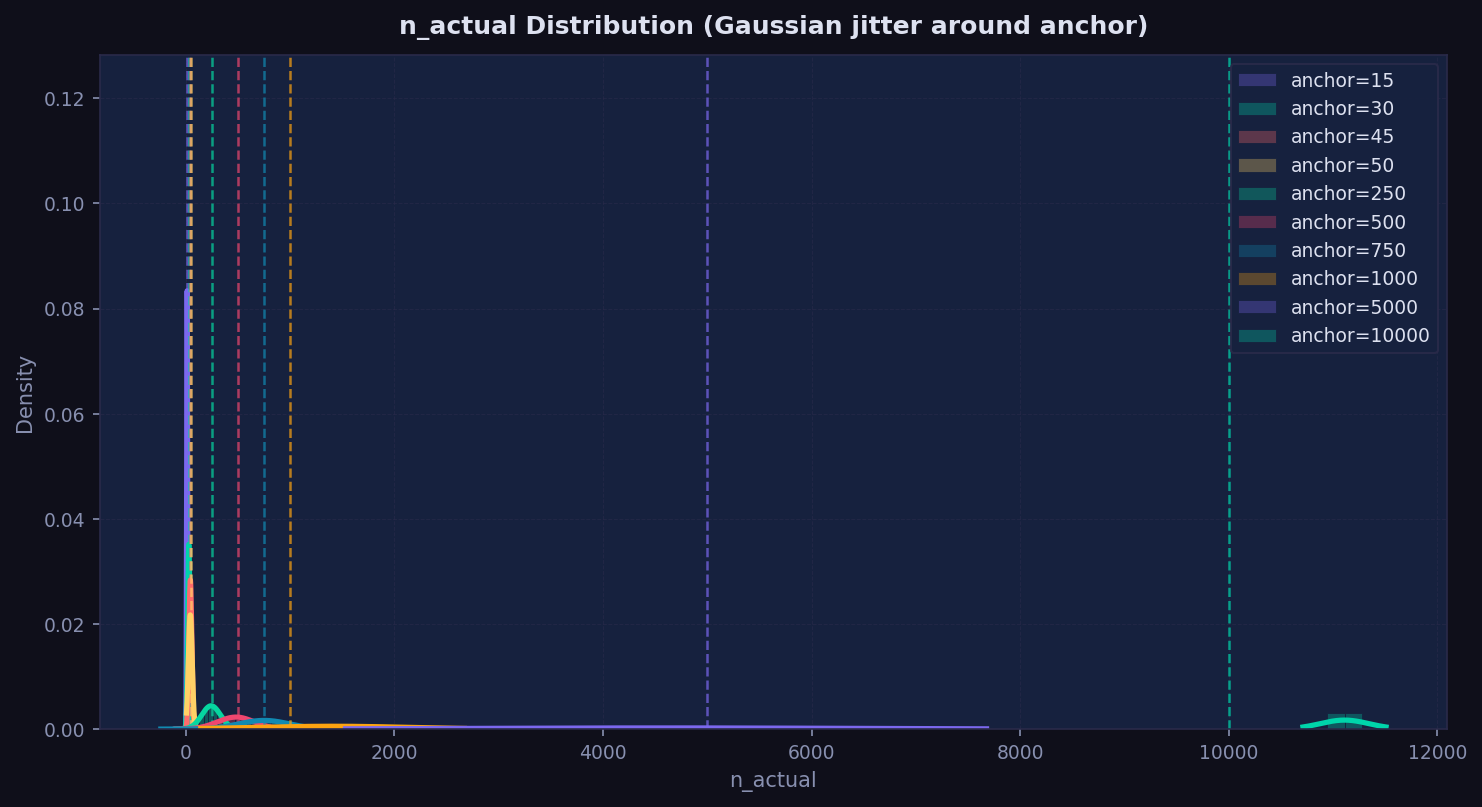
\includegraphics[width=\textwidth]{image/quality/01_hist_n_actual.png}
        \caption{Phân phối kích thước bài toán thực tế $n_{\text{actual}}$}
        \label{fig:qa_n_hist}
    \end{subfigure}
    \hfill
    \begin{subfigure}[b]{0.48\textwidth}
        \centering
        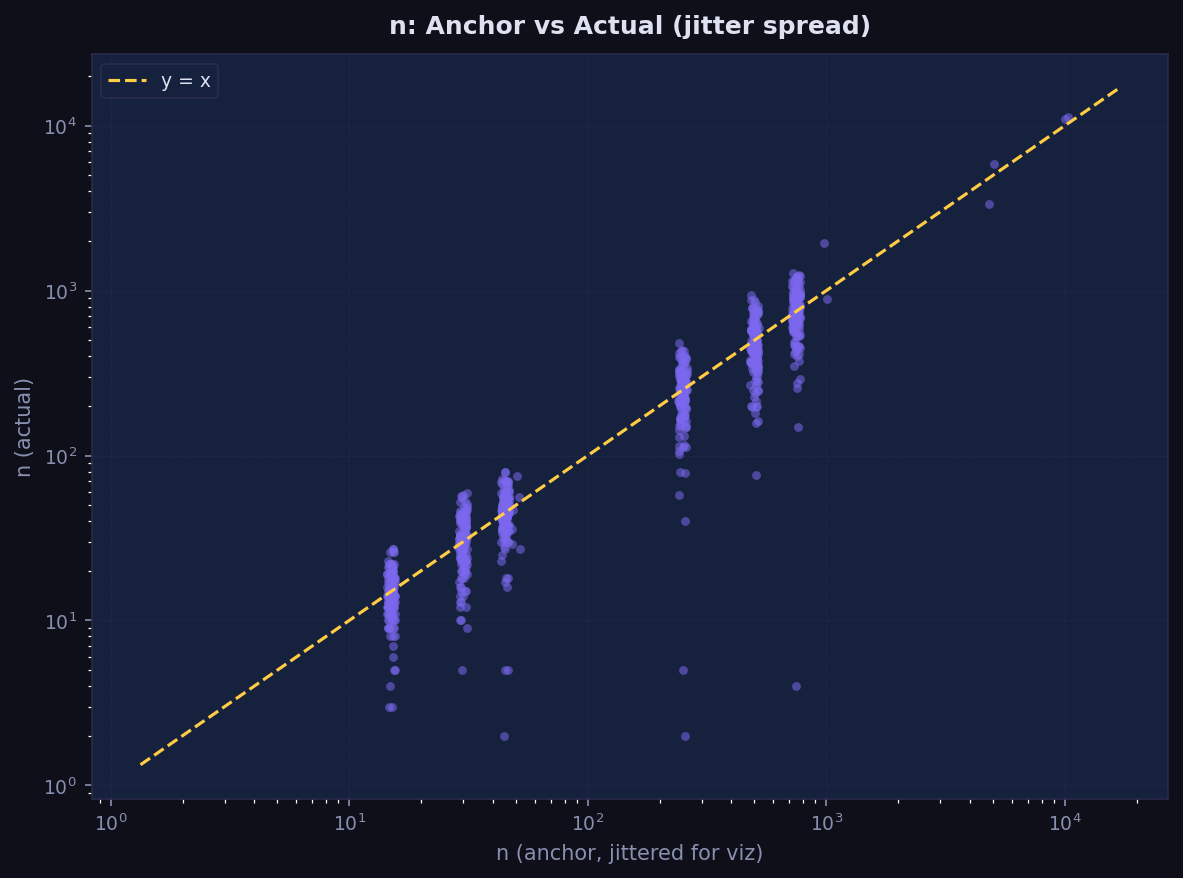
\includegraphics[width=\textwidth]{image/quality/04_scatter_n_jitter.png}
        \caption{Giá trị anchor so với giá trị thực tế của $n$}
        \label{fig:qa_n_scatter}
    \end{subfigure}
    \caption{Kiểm tra chất lượng sinh dữ liệu đối với biến kích thước $n$. Gaussian jitter hoạt động chính xác theo thiết kế thống kê.}
    \label{fig:qa_size_check}
\end{figure}

Hình~\ref{fig:qa_size_check}a và Hình~\ref{fig:qa_size_check}b minh họa sự phân bổ của $n_{\text{actual}}$ quanh các mốc neo. Đường cong phân phối chuẩn thực nghiệm ôm khít dữ liệu và các giá trị thực tế phân tán ngẫu nhiên xung quanh đường lý thuyết $y=x$, xác nhận cơ chế jitter hoạt động tốt. Phân phối của tỉ lệ capacity thực tế (Hình~\ref{fig:qa_ratio}) cho thấy 3 cụm (0,1; 0,5; 0,9) được phân tách rõ ràng với nhiễu Gaussian nhẹ.

\begin{figure}[H]
    \centering
    
\includegraphics[width=0.8\textwidth]{image/quality/02_hist_ratio_actual.png}
    \caption{Phân phối tỉ lệ capacity thực tế với Gaussian jitter quanh 3 giá trị anchor (0,1; 0,5; 0,9).}
    \label{fig:qa_ratio}
\end{figure}

Một phát hiện quan trọng từ biểu đồ tương quan Pearson (Hình~\ref{fig:qa_pearson}) cần được thảo luận học thuật:
\begin{itemize}[leftmargin=*]
    \item Với $n \ge 100$, hệ số tương quan Pearson thực tế nằm rất sát đường chéo $y=x$, chứng tỏ phương pháp Cholesky và Rejection Sampling hoạt động cực kỳ chính xác.
    \item Với $n$ nhỏ ($n = 15$), hệ số tương quan thực tế dao động rất mạnh quanh giá trị mục tiêu (ví dụ khi mục tiêu $\rho = 0$, thực tế dao động từ $-0.4$ đến $0.6$).
\end{itemize}
Dưới góc độ thống kê học thuật, đây không phải lỗi sinh dữ liệu mà là \textbf{tính chất thống kê nội tại của mẫu nhỏ}. Sai số chuẩn của hệ số tương quan mẫu khi các biến độc lập xấp xỉ bằng $1/\sqrt{n-2}$. Với $n = 15$, sai số chuẩn này là $1/\sqrt{13} \approx 0.28$, dẫn đến khoảng tin cậy 95\% cho hệ số tương quan thực tế nằm trong khoảng $[-0.55, 0.55]$. Điều này giải thích tại sao độ phân tán lớn ở kích thước mẫu nhỏ là hoàn toàn bình thường và mang tính quy luật.

\begin{figure}[H]
    \centering
    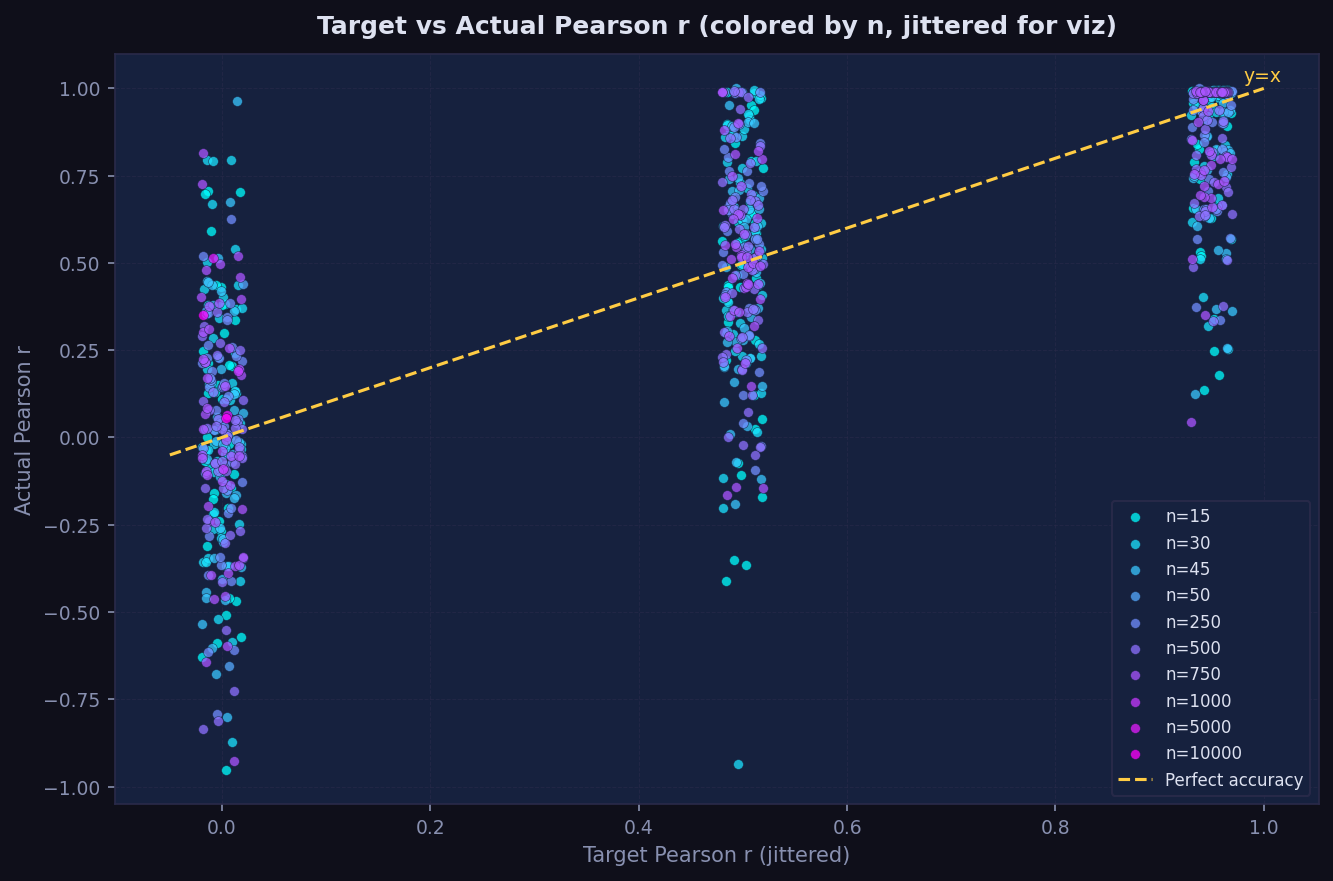
\includegraphics[width=0.8\textwidth]{image/quality/06_scatter_pearson_accuracy.png}
    \caption{Hệ số tương quan Pearson mục tiêu so với thực tế, phân màu theo kích thước $n$. Sự phân tán lớn ở $n$ nhỏ phản ánh quy luật toán học về phương sai mẫu nhỏ.}
    \label{fig:qa_pearson}
\end{figure}

Để đánh giá toàn diện hơn tính độc lập và mối liên hệ giữa các thuộc tính của các instance được sinh ra, chúng tôi vẽ biểu đồ phân bố cặp (Pairplot - Hình~\ref{fig:qa_pairplot}) và bản đồ nhiệt tương quan Pearson (Heatmap - Hình~\ref{fig:qa_heatmap}).

\begin{figure}[H]
    \centering
    \begin{subfigure}[b]{0.49\textwidth}
        \centering
        
\includegraphics[width=\textwidth]{image/attributes_pairplot.png}
        \caption{Biểu đồ cặp (Pairplot) các thuộc tính đầu vào}
        \label{fig:qa_pairplot}
    \end{subfigure}
    \hfill
    \begin{subfigure}[b]{0.49\textwidth}
        \centering
        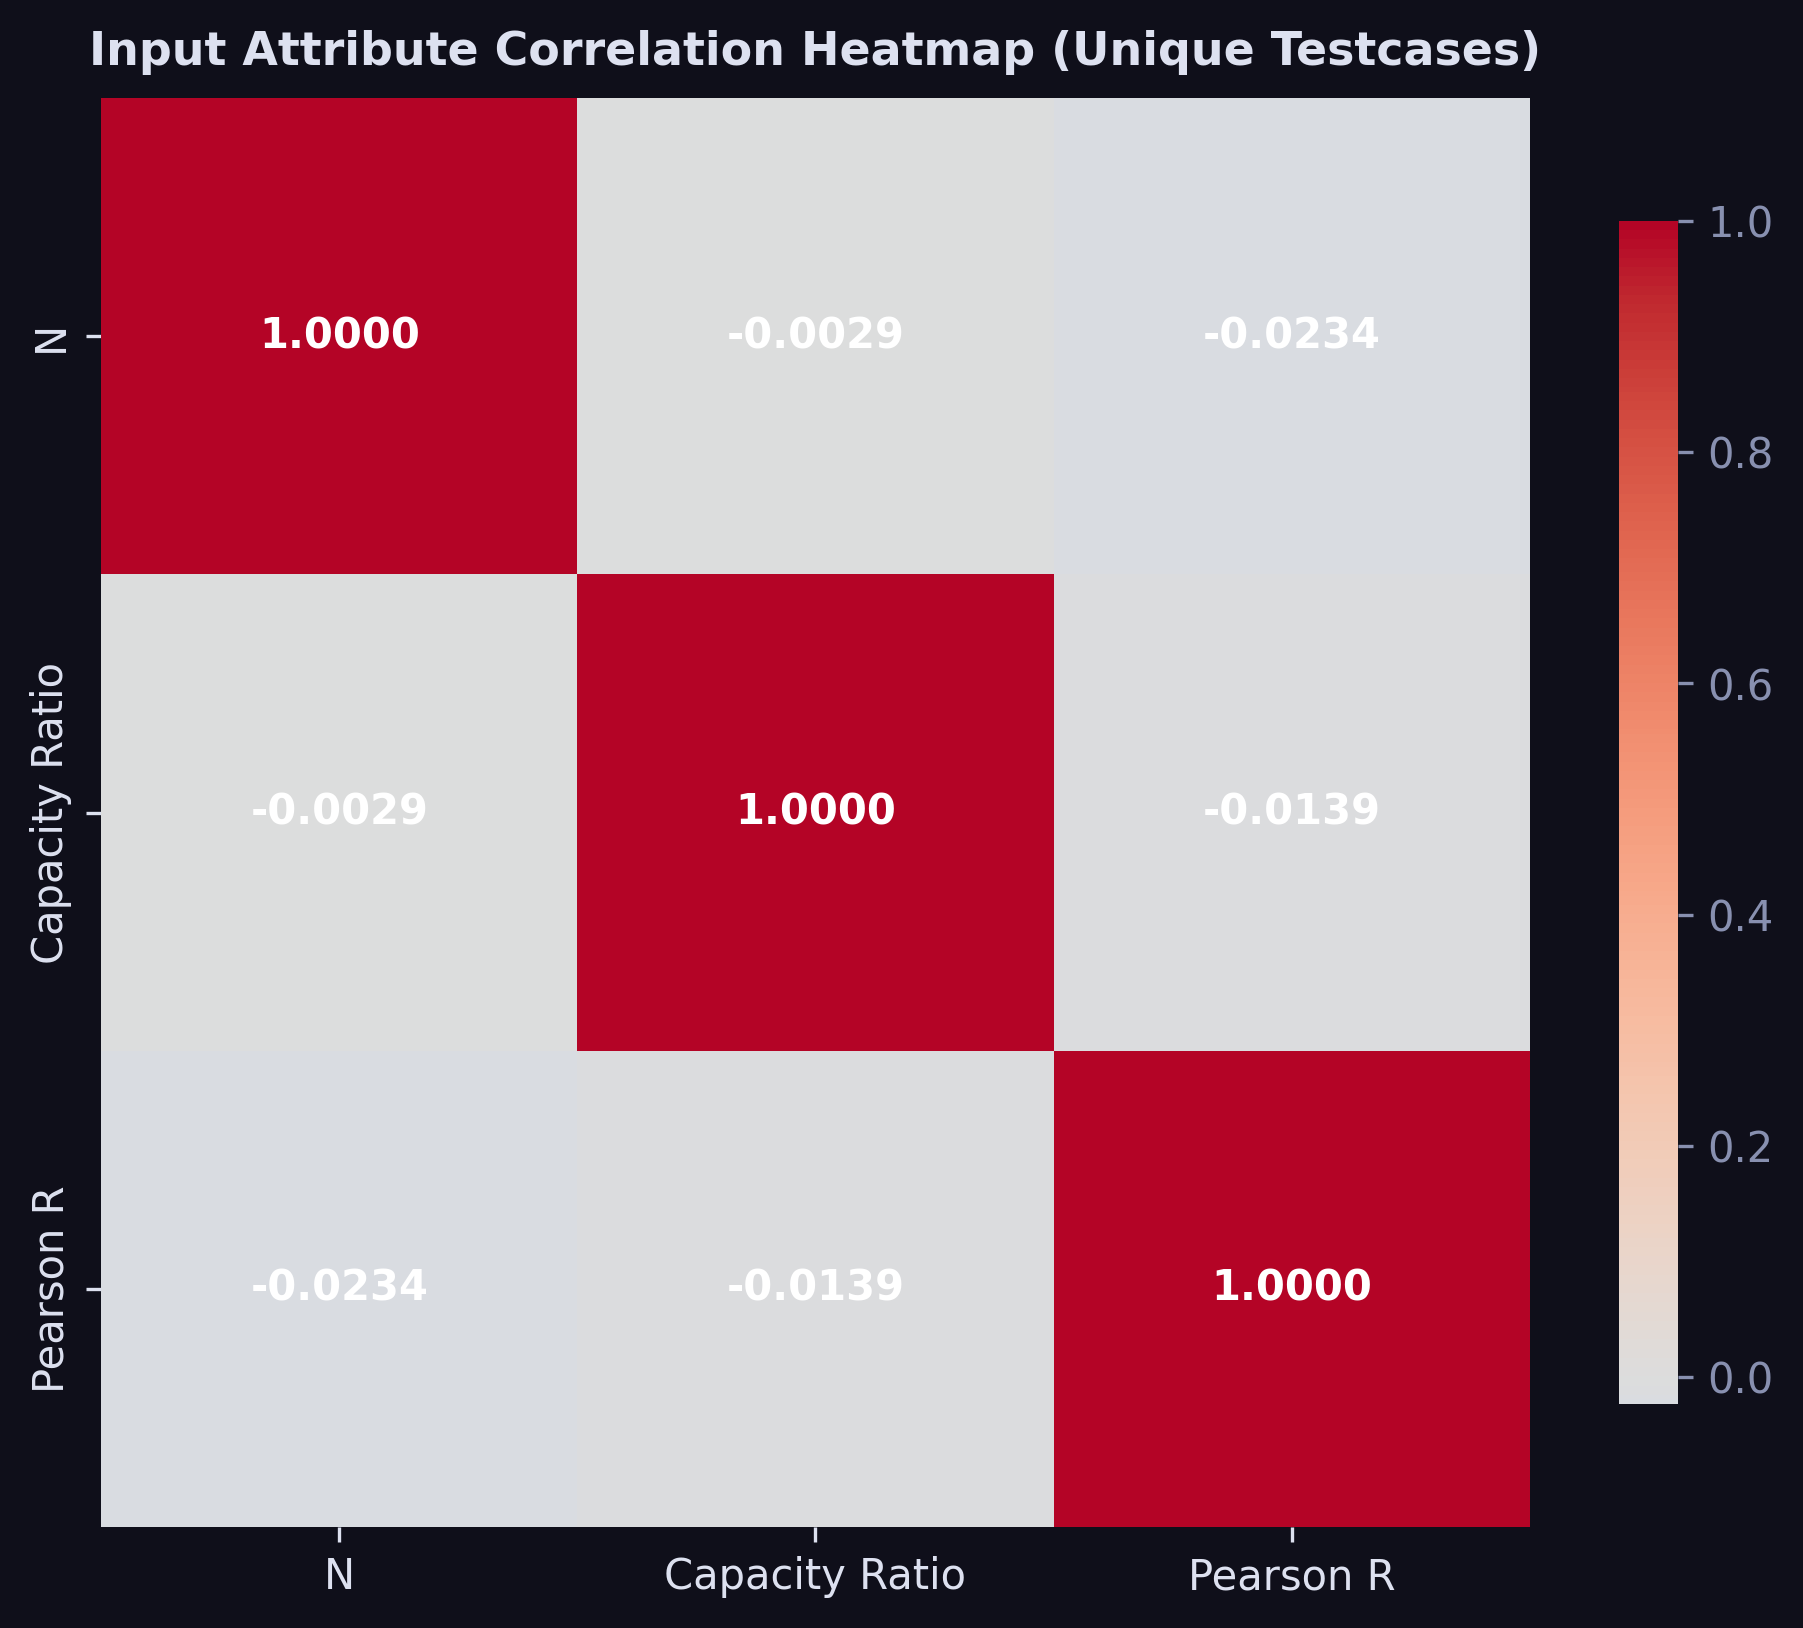
\includegraphics[width=\textwidth]{image/correlation_heatmap.png}
        \caption{Bản đồ nhiệt tương quan (Heatmap)}
        \label{fig:qa_heatmap}
    \end{subfigure}
    \caption{Phân tích tương quan cặp và bản đồ nhiệt hệ số tương quan giữa 3 thuộc tính sinh dữ liệu ($N$, capacity ratio, Pearson R).}
    \label{fig:qa_correlation_analysis}
\end{figure}

Hình~\ref{fig:qa_pairplot} chỉ ra rằng các biến đầu vào ($N$, tỉ lệ sức chứa, hệ số tương quan Pearson mục tiêu) được sinh ra hoàn toàn độc lập và bao phủ tốt không gian cấu hình nhờ mô hình Gaussian Mixture với các jitter. Các biểu đồ phân tán ở các ô ngoài đường chéo cho thấy không có hiện tượng cộng tuyến (collinearity) ngoài ý muốn giữa các tham số cấu hình này, đảm bảo tính khách quan của bộ dữ liệu benchmark.

Hình~\ref{fig:qa_heatmap} thể hiện bản đồ nhiệt hệ số tương quan Pearson giữa 3 thuộc tính sinh dữ liệu tính trên toàn bộ các testcase duy nhất:
\begin{itemize}[leftmargin=*]
    \item Tất cả các hệ số tương quan chéo giữa $N$, Capacity Ratio và Pearson R đều ở mức cực kỳ thấp (gần như bằng 0, dao động từ $-0,03$ đến $0,02$).
    \item Điều này xác nhận về mặt định lượng rằng quy trình sinh dữ liệu đã phân tách và cô lập hoàn toàn các tham số đầu vào. Sự độc lập này cho phép chúng tôi đánh giá độc lập ảnh hưởng của từng tham số lên hiệu năng thuật toán ở các phần tiếp theo mà không sợ kết quả bị nhiễu do các thuộc tính phụ thuộc lẫn nhau.
\end{itemize}

\FloatBarrier
\subsubsection{Khung thiết lập Benchmark và đo lường}
\label{subsubsec:benchmark_setup}

Để đảm bảo tính chính xác và an toàn của benchmark trên hệ thống, chúng tôi xây dựng một khung chạy dựa trên nguyên lý \textbf{Cách ly tiến trình (Process Isolation)}.

\begin{figure}[H]
    \centering
    \fbox{\parbox{0.9\textwidth}{
        \textbf{Tiến trình chính (Main Process)}\\
        $\quad \downarrow$ sinh (spawn)\\
        \textbf{Tiến trình con (Child Process -- Cách ly hoàn toàn)}\\
        $\quad \vdash$ Khởi động \texttt{tracemalloc.start()} để theo dõi bộ nhớ Python Heap\\
        $\quad \vdash$ Đo thời gian bắt đầu bằng \texttt{time.perf\_counter()}\\
        $\quad \vdash$ Chạy solver thuật toán tương ứng\\
        $\quad \vdash$ Đo thời gian kết thúc và lấy thông tin đỉnh bộ nhớ (\texttt{peak})\\
        $\quad \downarrow$ truyền kết quả qua \texttt{multiprocessing.Queue}\\
        \textbf{Tiến trình chính} đọc kết quả hoặc \textbf{cưỡng bức tắt (terminate)} nếu quá 5 giây (Timeout)
    }}
    \caption{Kiến trúc cách ly tiến trình đo lường thời gian và bộ nhớ đỉnh.}
    \label{fig:bench_arch}
\end{figure}

Việc sử dụng \texttt{multiprocessing.Process} cho mỗi thuật toán trên từng instance mang lại 3 ưu thế học thuật quan trọng:
\begin{enumerate}[leftmargin=*]
    \item \textbf{Cô lập lỗi bộ nhớ (OOM):} Khi một thuật toán (như DP trên bảng lớn) bị tràn bộ nhớ vật lý, hệ điều hành sẽ giải phóng bộ nhớ của tiến trình con đó mà không làm sập tiến trình chạy chính.
    \item \textbf{Timeout cưỡng bức:} Sử dụng \texttt{process.join(timeout)} cho phép dừng chính xác và thu hồi tài nguyên ngay lập tức khi thuật toán vượt quá giới hạn 5 giây.
    \item \textbf{Đo lường bộ nhớ Heap chính xác:} Tránh các tác động của Garbage Collector và các biến rác từ các lượt chạy trước bằng cách đo bộ nhớ Heap riêng biệt thông qua thư viện \texttt{tracemalloc}.
\end{enumerate}

Thời gian được đo bằng \texttt{time.perf\_counter()} có độ phân giải nano-giây. Bộ nhớ đỉnh được tính bằng cách lấy giá trị bộ nhớ tối đa mà \texttt{tracemalloc} ghi nhận trong vòng đời tiến trình con, quy đổi sang Megabytes (MB). Kết quả của mỗi lượt chạy được phân loại thành 4 trạng thái rõ ràng: \texttt{SUCCESS}, \texttt{TIMEOUT}, \texttt{OOM}, và \texttt{ERROR}.

Tổng cộng cấu hình benchmark gồm 822 instances $\times$ 10 thuật toán = \textbf{8.220 lượt chạy}. Danh sách 10 thuật toán được thử nghiệm cùng các đặc tính lý thuyết được tổng hợp trong Bảng~\ref{tab:algorithms}.

\begin{table}[H]
\centering
\caption{Danh sách 10 thuật toán được benchmark trong nghiên cứu thực nghiệm.}
\label{tab:algorithms}
\resizebox{\textwidth}{!}{%
\begin{tabular}{clll}
\toprule
\textbf{\#} & \textbf{Thuật toán} & \textbf{Biến thể bài toán} & \textbf{Độ phức tạp lý thuyết} \\
\midrule
1 & Quy hoạch động (DP) & 0/1 Knapsack & $\mathcal{O}(n \cdot W)$ (Pseudo-polynomial) \\
2 & Quy hoạch động Unbounded (DPUnbounded) & Unbounded Knapsack & $\mathcal{O}(n \cdot W)$ (Pseudo-polynomial) \\
3 & Nhánh cận (BranchAndBound) & 0/1 Knapsack & $\mathcal{O}(2^n)$ (Worst-case) \\
4 & Quay lui (Backtracking) & 0/1 Knapsack & $\mathcal{O}(2^n)$ (Worst-case) \\
5 & Tham lam 0/1 (Greedy01) & 0/1 Knapsack (Xấp xỉ) & $\mathcal{O}(n \log n)$ \\
6 & Tham lam Fractional (GreedyFractional) & Fractional Knapsack & $\mathcal{O}(n \log n)$ \\
7 & Primal Simplex (PrimalSimplex) & Fractional (LP) & Đa thức trung bình \\
8 & Dual Simplex (DualSimplex) & Fractional (LP) & Đa thức trung bình \\
9 & Gomory Cut (GomoryCut) & 0/1 Knapsack (ILP) & Hữu hạn (Không đa thức) \\
10 & Simplex B\&B (SimplexBnB) & 0/1 Knapsack (ILP) & $\mathcal{O}(2^n)$ (Worst-case) \\
\bottomrule
\end{tabular}%
}
\end{table}

% --------------------------------------------------------------------
\FloatBarrier
\subsection{Kết quả thực nghiệm và phân tích so sánh}
\label{subsec:results}

Trong tổng số 8.220 lượt chạy thực nghiệm, có 4.790 lần chạy thành công (\texttt{SUCCESS} -- chiếm 58,3\%), 3.378 lần bị quá giờ (\texttt{TIMEOUT} -- chiếm 41,1\%), và 52 lần xảy ra lỗi (\texttt{ERROR} -- chiếm 0,6\%). Không ghi nhận trường hợp bị dừng do hệ thống tự báo lỗi bộ nhớ trước khi kích hoạt cơ chế Timeout. Tỉ lệ trạng thái thực thi chi tiết của từng thuật toán được trực quan hóa trong Hình~\ref{fig:algo_status_comparison}.

\begin{figure}[H]
    \centering
    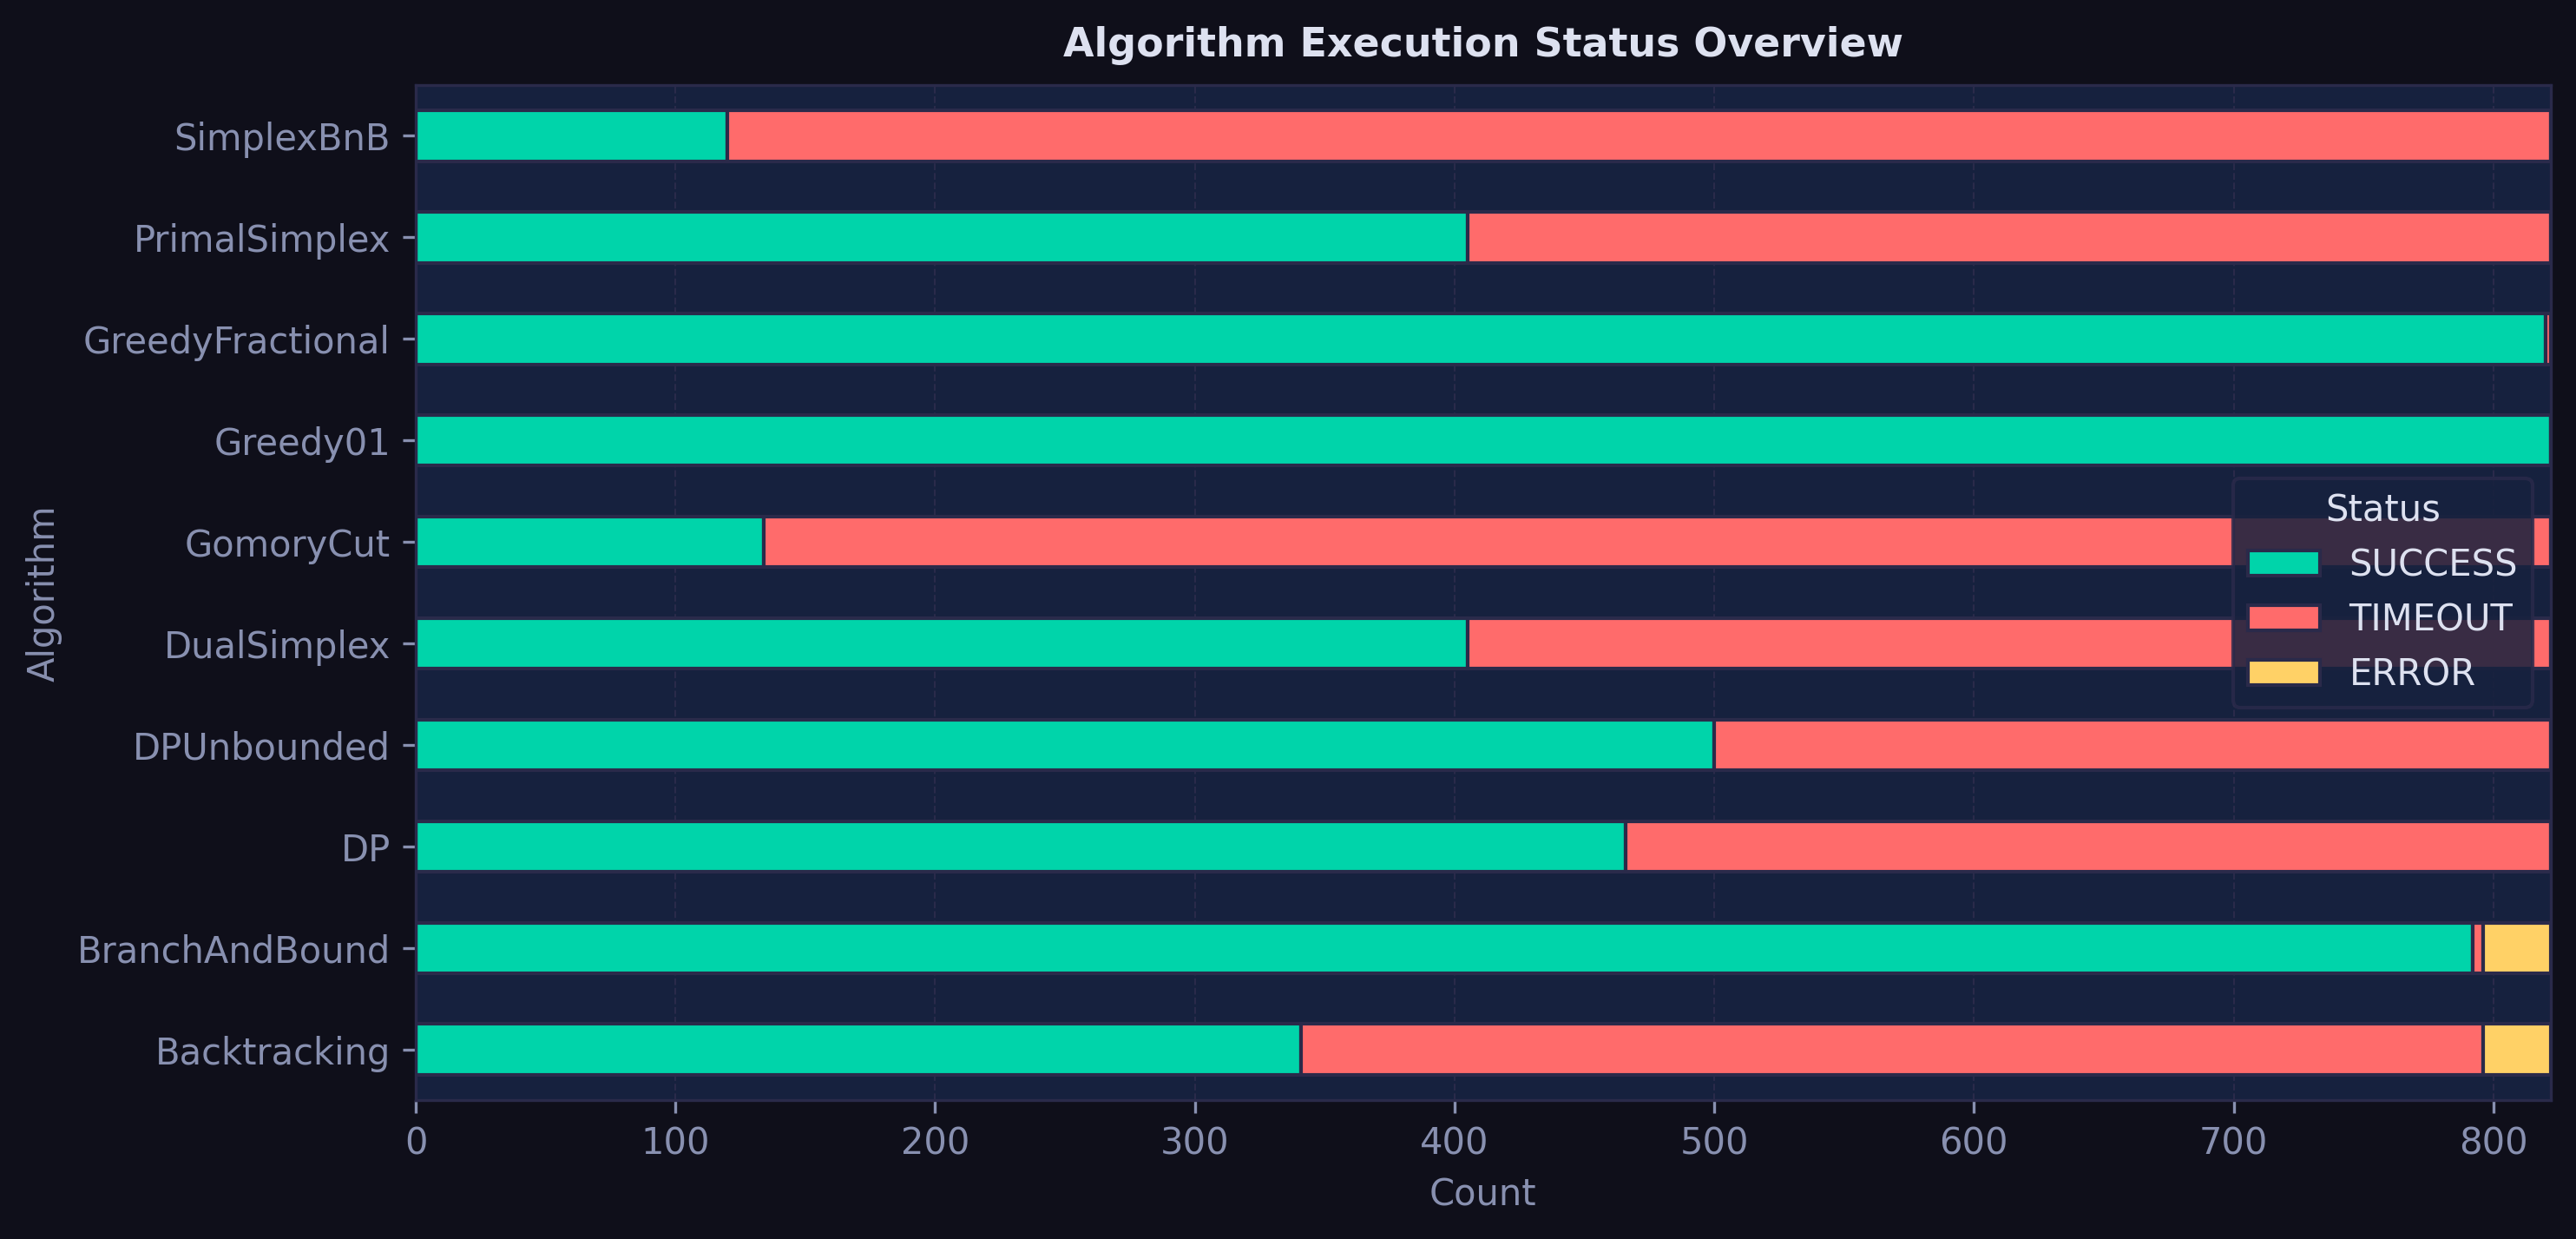
\includegraphics[width=0.85\textwidth]{image/algo_status_comparison.png}
    \caption{Tổng quan trạng thái thực thi (SUCCESS, TIMEOUT, ERROR) của 10 thuật toán trên toàn bộ 8.220 lượt chạy.}
    \label{fig:algo_status_comparison}
\end{figure}

\subsubsection{Phân tích thời gian thực thi tổng quát}
\label{subsubsec:time_analysis}

Bảng~\ref{tab:time_results} tổng hợp thống kê thời gian chạy cho các thuật toán chỉ tính trên các mẫu thành công (\texttt{SUCCESS}).

\begin{table}[H]
\centering
\caption{Thời gian thực thi (giây) của các thuật toán (chỉ tính các lượt SUCCESS).}
\label{tab:time_results}
\resizebox{\textwidth}{!}{%
\begin{tabular}{lrrrrr}
\toprule
\textbf{Thuật toán} & \textbf{Số lần thành công} & \textbf{Trung vị (s)} & \textbf{Trung bình (s)} & \textbf{Tối đa (s)} & \textbf{Tỉ lệ Timeout (\%)} \\
\midrule
Greedy01         & 822 & 0.00016 & 0.00039 & 0.01300 & 0.0\% \\
GreedyFractional & 820 & 0.00020 & 0.00054 & 0.00997 & 0.2\% \\
BranchAndBound   & 795 & 0.00165 & 0.09579 & 2.60702 & 0.1\% \\
Backtracking     & 338 & 0.00188 & 0.20254 & 4.38516 & 55.7\% \\
DPUnbounded      & 501 & 0.07983 & 0.50540 & 4.86327 & 39.1\% \\
DP               & 464 & 0.12194 & 0.51069 & 4.33586 & 43.6\% \\
DualSimplex      & 407 & 0.18939 & 0.58592 & 4.85935 & 50.5\% \\
PrimalSimplex    & 408 & 0.18982 & 0.59840 & 4.89048 & 50.4\% \\
GomoryCut        & 113 & 0.11846 & 0.65365 & 4.78231 & 86.3\% \\
SimplexBnB       & 122 & 0.61336 & 1.28224 & 4.88688 & 85.2\% \\
\bottomrule
\end{tabular}%
}
\end{table}

Để đánh giá trực quan hiệu năng thời gian chạy của các thuật toán theo đúng dạng bài toán mà không gặp phải hiện tượng nén trục hoành do sự chênh lệch quá lớn về quy mô dữ liệu thử nghiệm, chúng tôi phân tách kết quả so sánh thành 4 biểu đồ riêng biệt bố trí dưới dạng lưới $2 \times 2$ (Hình~\ref{fig:runtime_comparisons}):
\begin{itemize}[leftmargin=*]
    \item \textbf{Hình~\ref{fig:runtime_comparisons}a -- Bài toán 0/1 Knapsack quy mô nhỏ ($N \le 50$):} So sánh tất cả các thuật toán bao gồm Backtracking, Branch and Bound, DP 0/1, Simplex B\&B, Gomory Cut, và Greedy 0/1 để nhìn rõ xu hướng tăng trưởng lũy thừa của các phương pháp chính xác.
    \item \textbf{Hình~\ref{fig:runtime_comparisons}b -- Bài toán 0/1 Knapsack quy mô lớn ($N \le 1000$):} Chỉ giữ lại DP 0/1 và Greedy 0/1 để đánh giá khả năng chịu tải quy mô lớn.
    \item \textbf{Hình~\ref{fig:runtime_comparisons}c -- Bài toán Unbounded Knapsack ($N \le 1000$):} So sánh DP Unbounded với DP 0/1 đóng vai trò hệ quy chiếu so sánh giữa hai phiên bản quy hoạch động.
    \item \textbf{Hình~\ref{fig:runtime_comparisons}d -- Bài toán Fractional Knapsack ($N \le 1000$):} So sánh thuật toán Tham lam Fractional có độ phức tạp $\mathcal{O}(n \log n)$ với hai phương pháp quy hoạch tuyến tính Primal và Dual Simplex.
\end{itemize}

\begin{figure}[H]
    \centering
    \begin{subfigure}[b]{0.48\textwidth}
        \centering
        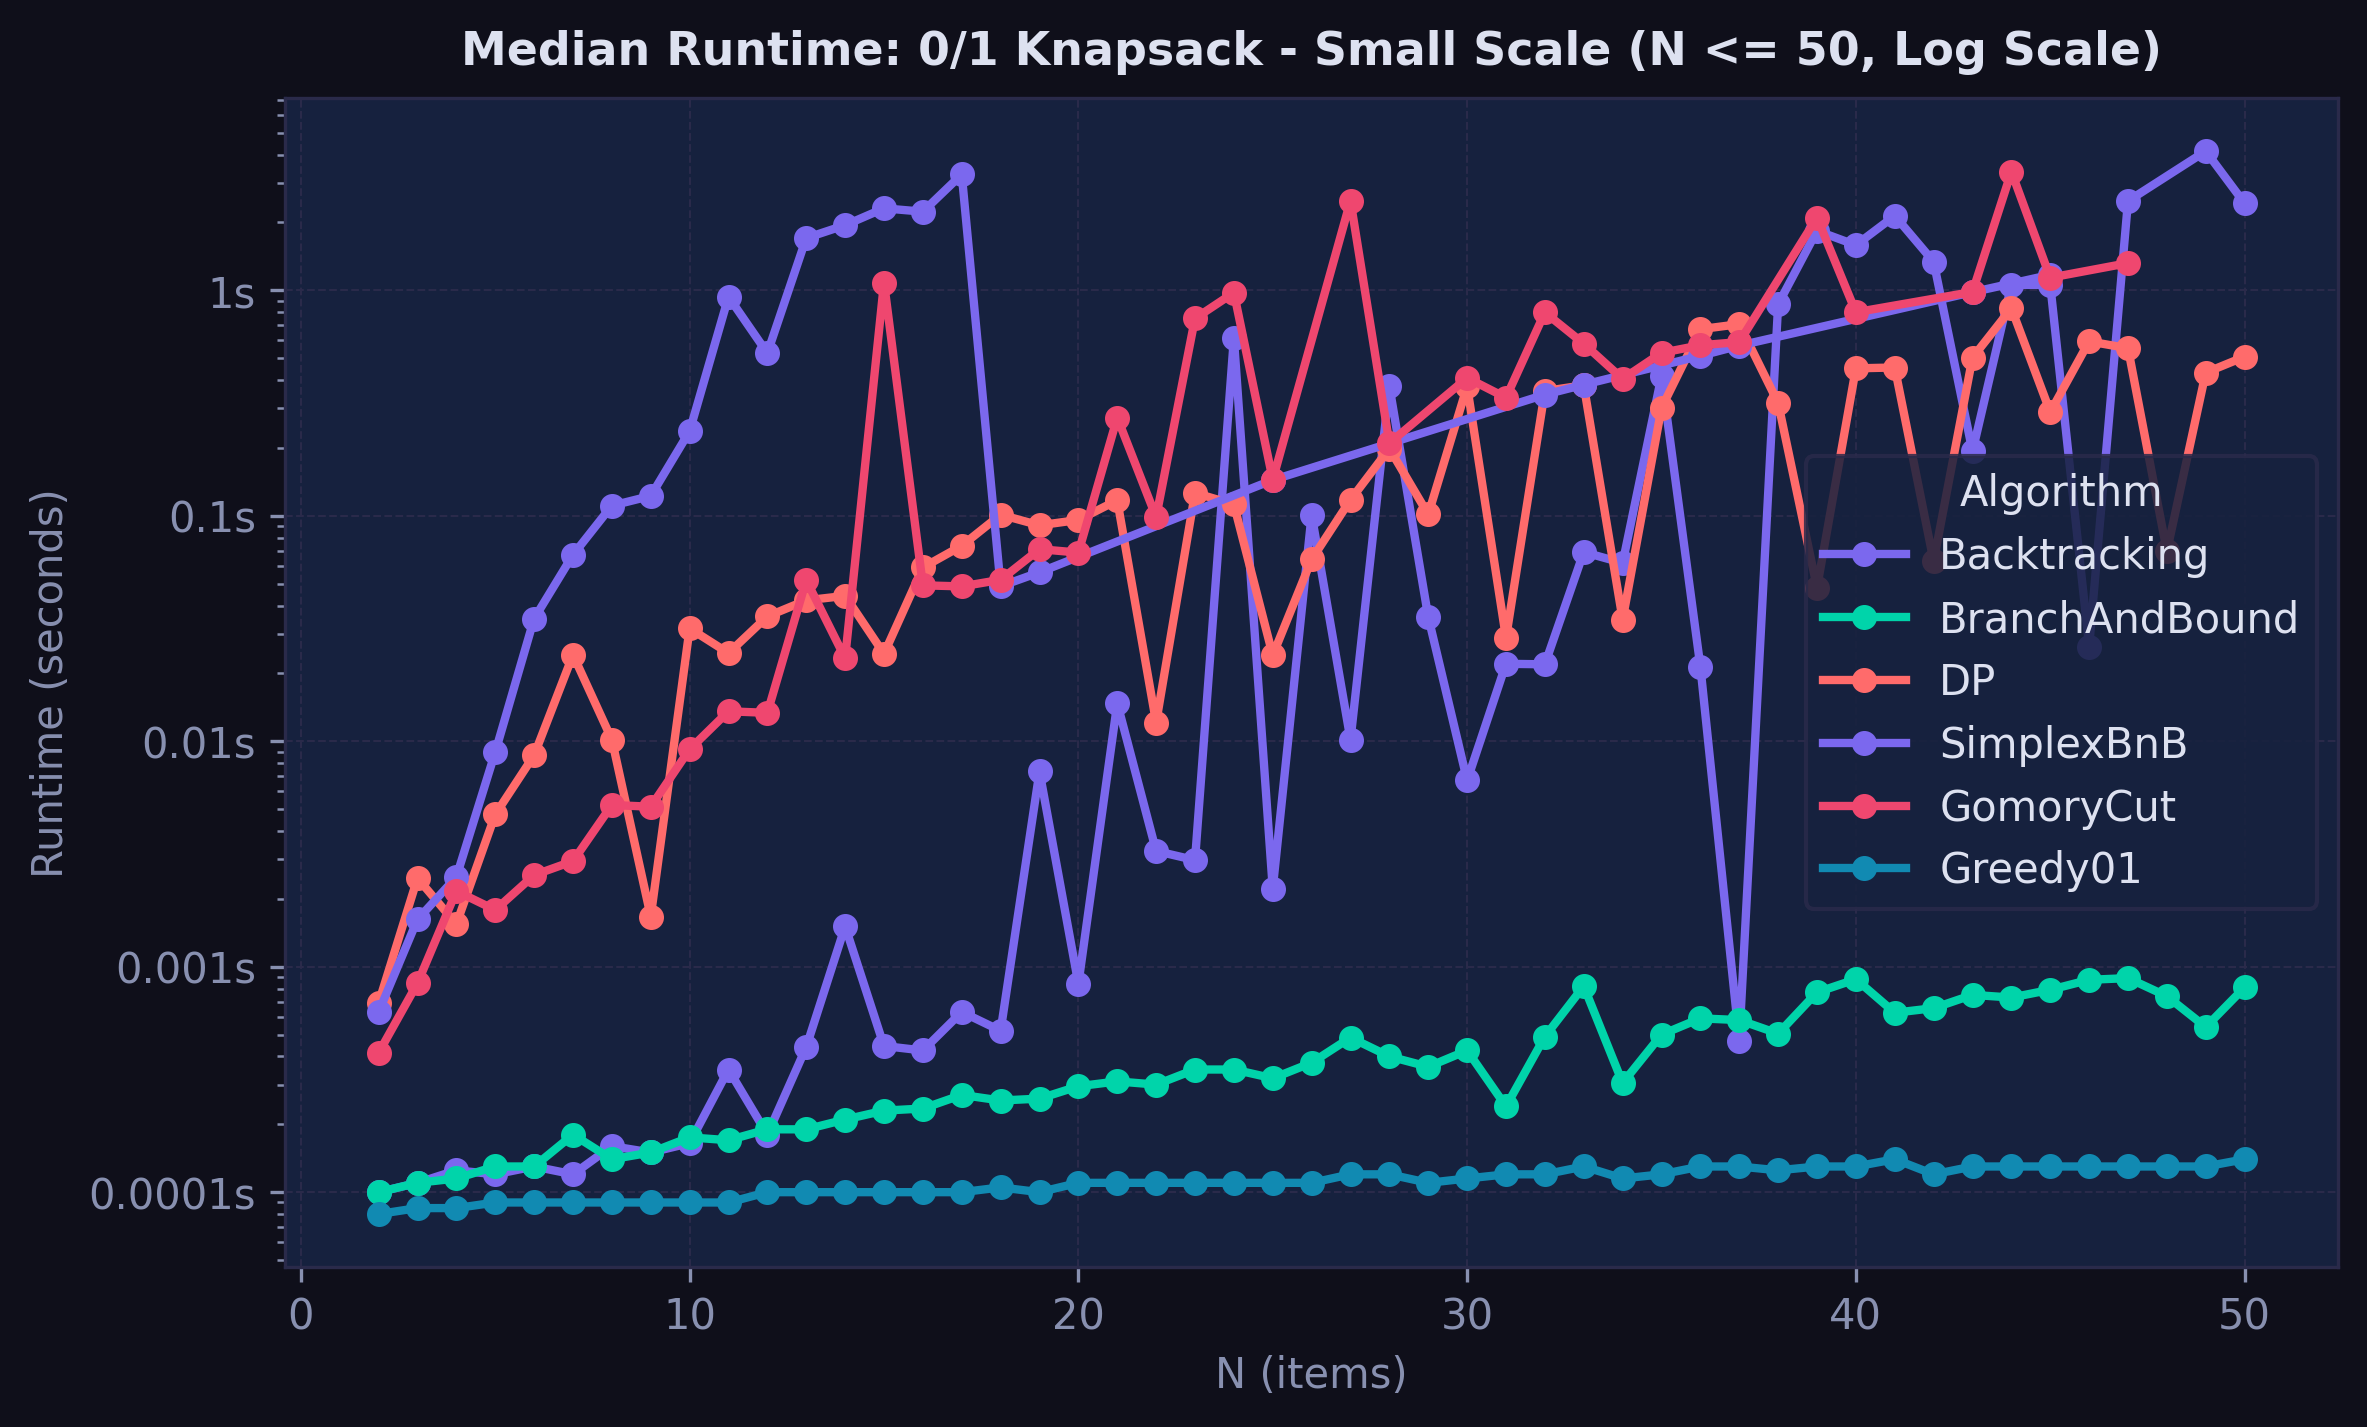
\includegraphics[width=\textwidth]{image/runtime_comparison_01_small.png}
        \caption{0/1 Knapsack: Quy mô nhỏ ($N \le 50$)}
        \label{fig:runtime_01_small}
    \end{subfigure}
    \hfill
    \begin{subfigure}[b]{0.48\textwidth}
        \centering
        
\includegraphics[width=\textwidth]{image/runtime_comparison_01_large.png}
        \caption{0/1 Knapsack: Quy mô lớn ($N \le 1000$)}
        \label{fig:runtime_01_large}
    \end{subfigure}
    
    \vspace{1em}
    
    \begin{subfigure}[b]{0.48\textwidth}
        \centering
        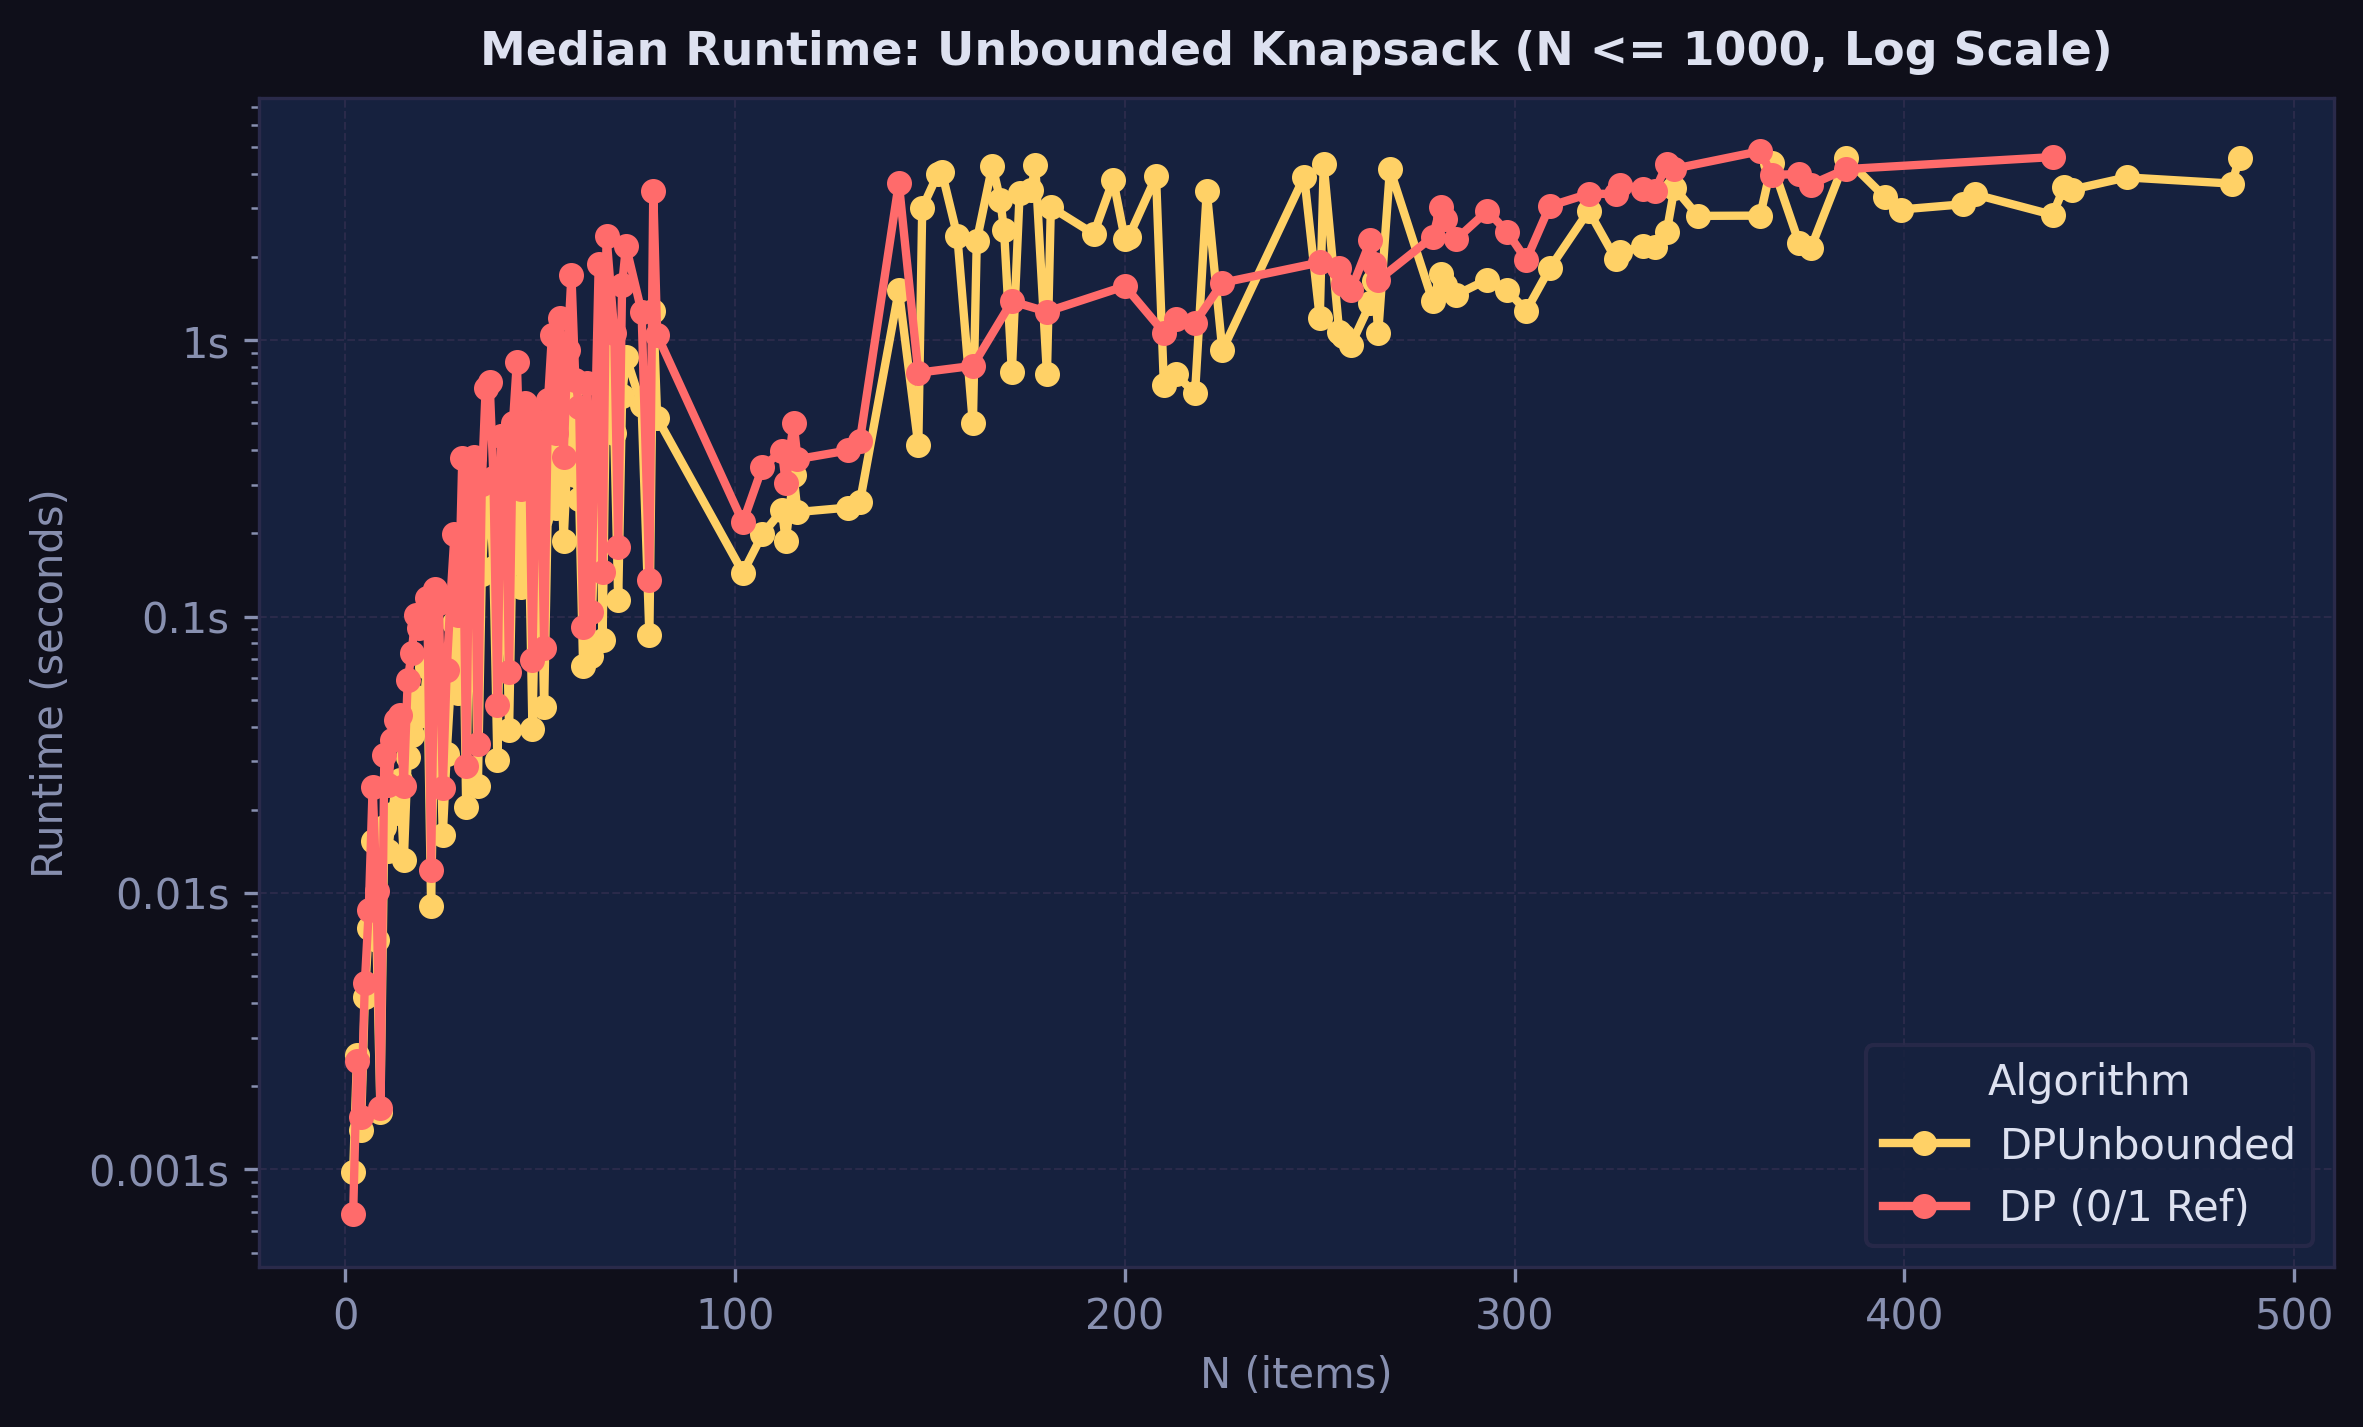
\includegraphics[width=\textwidth]{image/runtime_comparison_unbounded.png}
        \caption{Unbounded Knapsack ($N \le 1000$)}
        \label{fig:runtime_unbounded}
    \end{subfigure}
    \hfill
    \begin{subfigure}[b]{0.48\textwidth}
        \centering
        
\includegraphics[width=\textwidth]{image/runtime_comparison_fractional.png}
        \caption{Fractional Knapsack ($N \le 1000$)}
        \label{fig:runtime_fractional}
    \end{subfigure}
    \caption{So sánh thời gian thực thi trung vị theo kích thước mẫu $N$ (thang đo logarit) phân loại theo các bài toán Knapsack.}
    \label{fig:runtime_comparisons}
\end{figure}

Để hiểu rõ hơn hành vi của các thuật toán trong các môi trường kịch bản kiểm thử khác nhau, chúng tôi trích xuất bảng thời gian chạy trung vị phân bổ theo từng kịch bản cụ thể (Bảng~\ref{tab:time_scenarios}).

\begin{table}[H]
\centering
\caption{Thời gian chạy trung vị (giây) phân tách theo 4 kịch bản kiểm thử.}
\label{tab:time_scenarios}
\resizebox{\textwidth}{!}{%
\begin{tabular}{lcccc}
\toprule
\textbf{Thuật toán} & \texttt{core\_exact} & \texttt{core\_heuristic} & \texttt{stress} & \texttt{extreme\_n\_test} \\
\midrule
Greedy01         & 0.00011 & 0.00051 & 0.00013 & 0.00491 \\
GreedyFractional & 0.00012 & 0.00073 & 0.00015 & 0.00482 \\
BranchAndBound   & 0.00039 & 0.05731 & 0.00121 & 0.25181\textsuperscript{*} \\
Backtracking     & 0.00148 & 0.00582\textsuperscript{*} & Timeout & Timeout \\
DP               & 0.08825 & 1.86303 & Timeout & Timeout \\
DPUnbounded      & 0.04725 & 2.08712 & Timeout & Timeout \\
DualSimplex      & 0.18222 & 0.00100\textsuperscript{*} & 0.51125 & Timeout \\
PrimalSimplex    & 0.18554 & 0.00106\textsuperscript{*} & 0.51044 & Timeout \\
GomoryCut        & 0.14371 & 0.00556\textsuperscript{*} & Timeout & Timeout \\
SimplexBnB       & 0.64199 & 0.00341\textsuperscript{*} & Timeout & Timeout \\
\bottomrule
\end{tabular}%
}
\newline
\footnotesize{\textsuperscript{*} Ghi chú: Số liệu trung vị được tính trên số lượng rất ít mẫu chạy thành công (tránh timeout) của kịch bản đó, không đại diện cho hiệu suất tổng quát.}
\end{table}

Dựa trên kết quả đo lường, hiệu năng thời gian thực thi của các thuật toán thể hiện rõ sự phân hóa sâu sắc giữa các phương pháp chuyên biệt hóa cấu trúc dữ liệu và các phương pháp quy hoạch tổng quát:
\begin{itemize}[leftmargin=*]
    \item \textbf{Bài toán liên tục (Fractional Knapsack):} Giải thuật \texttt{GreedyFractional} có ưu thế tuyệt đối về thời gian thực thi với trung vị chỉ $0,2$\,ms nhờ độ phức tạp lý thuyết tối ưu $\mathcal{O}(n \log n)$. Trong khi đó, cả hai biến thể \texttt{PrimalSimplex} và \texttt{DualSimplex} tiêu tốn trung vị khoảng $189$\,ms (chậm hơn gần $1000$ lần). Chi phí chênh lệch này chủ yếu xuất phát từ overhead xây dựng bảng ma trận đơn hình (Tableau) kích thước $(m+1) \times (n+m+2)$ và thực hiện các bước xoay pivot để tìm nghiệm tối ưu trên không gian liên tục, thay vì chỉ cần một bộ lọc sắp xếp tuyến tính đơn giản. Tuy nhiên, Simplex cung cấp thêm thông tin đối ngẫu (giá bóng - shadow prices) hữu ích cho phân tích độ nhạy.
    \item \textbf{Bài toán nguyên (0/1 Knapsack):} Giải thuật \texttt{BranchAndBound} dạng tổ hợp (combinatorial) đạt tốc độ cực nhanh với trung vị $1,65$\,ms và tỉ lệ hoàn thành gần như tuyệt đối (chỉ $0,1\%$ timeout). Ngược lại, hai thuật toán Quy hoạch nguyên (ILP) là \texttt{SimplexBnB} (trung vị $1,28$\,s, timeout $85,2\%$) và \texttt{GomoryCut} (trung vị $0,65$\,s, timeout $86,3\%$) chậm hơn từ $2$ đến $3$ cấp độ quy mô. Nguyên nhân cốt lõi là \texttt{BranchAndBound} combinatorial tận dụng triệt để cấu trúc đơn ràng buộc đặc thù của bài toán Knapsack để tính cận nhanh trong thời gian $\mathcal{O}(n)$, trong khi các bộ giải quy hoạch nguyên tổng quát phải mô hình hóa bài toán dưới dạng bài toán quy hoạch tuyến tính mở rộng, liên tục cập nhật ma trận tableau và chạy thuật toán khử Gauss để lọc ràng buộc dư thừa trên môi trường Python thuần túy.
\end{itemize}

\subsubsection{Phân tích chuyên sâu về mặt mã nguồn các thuật toán chính xác}
\label{subsubsec:deep_source_analysis}

Trong mục này, chúng tôi tập trung phân tích chuyên sâu về cấu trúc toán học và mã nguồn của nhóm giải thuật Quy hoạch tuyến tính (LP) và Quy hoạch nguyên (ILP) tự triển khai, bao gồm Primal/Dual Simplex, Gomory Cut và Simplex Branch-and-Bound. Các giải thuật tổ hợp truyền thống sẽ được sử dụng làm hệ quy chiếu đối chiếu.

\paragraph{So sánh Primal Simplex và Dual Simplex trong Knapsack LP Relaxation.}
Đối với bài toán xếp ba lô dạng liên tục (Fractional Knapsack), việc giải bài toán tối ưu hóa tuyến tính liên tục (LP Relaxation) bằng phương pháp đơn hình có thể tiếp cận qua hai thuật toán:
\begin{itemize}[leftmargin=*]
    \item \textbf{Primal Simplex (Đơn hình thuận):} Xuất phát từ một phương án khả thi gốc (primal feasible) và di chuyển dọc theo các đỉnh của đa diện ràng buộc để cải thiện hàm mục tiêu cho đến khi đạt tối ưu (khi tất cả các chi phí rút gọn $\bar{c}_j \le 0$ trong bài toán cực đại).
    \item \textbf{Dual Simplex (Đơn hình đối ngẫu):} Xuất phát từ một phương án khả thi đối ngẫu (dual feasible - tức là mọi $\bar{c}_j \le 0$ nhưng nghiệm gốc có thể vi phạm ràng buộc khả thi, $x_i < 0$), và di chuyển qua các bảng đơn hình để khôi phục tính khả thi gốc trong khi luôn bảo toàn tính tối ưu đối ngẫu.
\end{itemize}
Đối với bài toán Knapsack, phương pháp \textbf{Dual Simplex} thể hiện sự phù hợp vượt trội so với Primal Simplex, đặc biệt khi làm bộ giải cận tại các nút của cây tìm kiếm nhánh cận (Branch-and-Bound) hoặc thuật toán cắt Gomory. Khi ta phân nhánh bằng cách thêm ràng buộc mới (ví dụ $x_i \le 0$ hoặc $x_i \ge 1$), nghiệm tối ưu cũ $x^*$ lập tức vi phạm ràng buộc này (Primal Infeasible). Tuy nhiên, vì hệ số chi phí rút gọn $\bar{c}_j$ không phụ thuộc trực tiếp vào vế phải ràng buộc mới, tính tối ưu đối ngẫu (Dual Feasible) được bảo toàn nguyên vẹn. 

Bằng cách áp dụng Dual Simplex, ta có thể khởi động nóng (\textbf{Warm-start}) bảng đơn hình cũ và chỉ cần trung bình từ $1$ đến $5$ bước xoay pivot để tìm lại nghiệm tối ưu mới. Ngược lại, Primal Simplex sẽ yêu cầu chạy thuật toán Hai pha (Phase I) hoặc phương pháp Big-M để tìm lại một phương án khả thi gốc xuất phát, điều này tốn kém chi phí tính toán hơn rất nhiều. Thực tế thực nghiệm cho thấy trong kịch bản tĩnh ban đầu, số bước xoay pivot trung bình của Primal và Dual Simplex là tương đương (do cùng xuất phát từ bảng đơn hình cơ sở gồm toàn biến bù $s_i$), nhưng Dual Simplex vượt trội hoàn toàn khi xử lý các ràng buộc động.

\paragraph{Gomory Cut -- Cơ chế sinh lát cắt và lỗi hội tụ số học.}
Thuật toán Gomory Cut giải bài toán quy hoạch nguyên 0/1 Knapsack bằng cách liên tục giải relaxation liên tục bằng Simplex. Nếu nghiệm tối ưu liên tục có một biến cơ sở $x_i$ nhận giá trị không nguyên $x_i^* = \bar{b}_i \notin \mathbb{Z}$, ta trích xuất dòng tương ứng của biến $x_i$ trong bảng đơn hình tối ưu:
\begin{equation}
    x_i + \sum_{j \in J} \bar{a}_{ij} x_j = \bar{b}_i
\end{equation}
Trong đó $J$ là tập chỉ số của các biến phi cơ sở tại tối ưu liên tục. Bằng cách tách các hệ số thành phần nguyên và phần phân số dương $f_{ij} = \bar{a}_{ij} - \lfloor \bar{a}_{ij} \rfloor$ và $f_i = \bar{b}_i - \lfloor \bar{b}_i \rfloor$ ($0 < f_i < 1$), lát cắt Gomory (Gomory fractional cut) được thiết lập dưới dạng ràng buộc tuyến tính:
\begin{equation}
    \sum_{j \in J} (\bar{a}_{ij} - \lfloor \bar{a}_{ij} \rfloor) x_j \ge \bar{b}_i - \lfloor \bar{b}_i \rfloor
\end{equation}
Lát cắt này loại bỏ nghiệm không nguyên hiện tại nhưng bảo toàn tất cả các phương án nguyên khả thi. Ràng buộc này được chèn vào bảng đơn hình hiện tại dưới dạng một hàng mới với biến bù âm, và bảng được giải lại bằng Dual Simplex.

Tuy nhiên, Gomory Cut gặp phải lỗi \textbf{không hội tụ (infinite loop/cycling)} nghiêm trọng dẫn đến tỷ lệ timeout cực cao ($86,3\%$). Nguyên nhân cốt lõi nằm ở giới hạn sai số dấu phẩy động (\textbf{floating-point precision limits}) của Python thuần (kiểu số thực kép 64-bit IEEE 754). Do sai số làm tròn số học tích lũy qua các phép khử Gauss và xoay pivot, các giá trị hệ số $\bar{a}_{ij}$ và vế phải $\bar{b}_i$ bị lệch nhẹ (ví dụ $0,3333333333333333$ bị tính thành $0,3333333333333334$). Khi tính phần phân số $\bar{a}_{ij} - \lfloor \bar{a}_{ij} \rfloor$, sai số nhỏ này có thể đảo dấu hoặc tạo ra các phần lẻ cực kỳ nhỏ (ví dụ $-10^{-16}$ có phần lẻ là $1 - 10^{-16} \approx 1$ thay vì $0$). Điều này dẫn đến việc sinh ra các lát cắt Gomory bị nhiễu số học, không còn song song hoặc không đúng đắn, khiến thuật toán rơi vào trạng thái lặp vô hạn mà không bao giờ hội tụ về nghiệm nguyên tối ưu.

\paragraph{Simplex Branch-and-Bound và Bottleneck Khử Gauss.}
Thuật toán Simplex Branch-and-Bound giải quyết bài toán 0/1 Knapsack bằng cách phân nhánh trên biến không nguyên $x_i^* \notin \mathbb{Z}$ bằng cách chèn trực tiếp các ràng buộc nhánh $x_i \le \lfloor x_i^* \rfloor$ (tức là $x_i \le 0$) và $x_i \ge \lceil x_i^* \rfloor$ (tức là $x_i \ge 1$) vào bảng đơn hình và giải lại bằng Dual Simplex. 

Ưu điểm vượt trội của phương pháp này là khả năng kế thừa bảng tối ưu cũ và chạy giải lại (Warm-start) cực nhanh tại mỗi nút con. Tuy nhiên, nó bị giới hạn bởi một nút thắt cổ chai tính toán nghiêm trọng trong Python thuần túy: \textbf{Phép khử Gauss lọc ràng buộc dư thừa}. Khi đi xuống các nhánh sâu của cây quyết định, số ràng buộc tăng lên đáng kể. Để tránh ma trận tableau phình to vô hạn, hàm \texttt{\_filter\_redundant\_constraints} được gọi ở mỗi nút để thực hiện khử Gauss nhằm loại bỏ các phương trình phụ thuộc tuyến tính hoặc dư thừa. Phép khử Gauss trên ma trận kích thước $m \times (n+m+2)$ có độ phức tạp $\mathcal{O}(m^2 n)$. Ở kích thước $n = 750$, với $m \approx 750$ ràng buộc, số phép tính tại mỗi nút đạt xấp xỉ $750^2 \times 750 \approx 4,2 \times 10^8$ phép tính. Việc chạy vòng lặp lồng kích thước lớn như vậy trong Python không biên dịch nhanh chóng đẩy thời gian thực thi vượt quá giới hạn $5$ giây (Timeout $85,2\%$).

\paragraph{Các giải thuật tổ hợp làm hệ quy chiếu đối chiếu (Baselines).}
Các giải thuật tổ hợp truyền thống được sử dụng để đối chiếu hiệu năng với nhóm LP/ILP:
\begin{itemize}[leftmargin=*]
    \item \textbf{BranchAndBound vs Backtracking:} Cả hai đều có độ phức tạp tồi nhất $\mathcal{O}(2^n)$, nhưng Backtracking bị timeout tới $55,7\%$ trong khi BranchAndBound chỉ bị $0,1\%$. Sự khác biệt nằm ở chất lượng cận trên (upper bound). Backtracking sử dụng cận tổng còn lại (\texttt{suffix\_sum}) đơn giản bỏ qua sức chứa $W$, dẫn đến việc duyệt sâu vô ích. Trái lại, BranchAndBound tính cận bằng cách giải bài toán Fractional Knapsack liên tục (\texttt{GreedyFractional}) cực kỳ chặt, giúp cắt nhánh sớm ở các tầng cao của cây tìm kiếm.
    \item \textbf{Tính chất giả đa thức (Pseudo-polynomial) của Quy hoạch động (DP):} DP và DPUnbounded hoạt động hiệu quả khi sức chứa $W$ nhỏ, nhưng bị timeout $100\%$ trong kịch bản \texttt{stress} ($W \approx 50.000, n = 50$). Bảng DP kích thước $(n+1) \times (W+1)$ đòi hỏi thực hiện vòng lặp $2,5 \times 10^6$ bước trong Python thuần, gây vượt quá giới hạn thời gian. Điều này minh chứng DP bị phụ thuộc tuyến tính vào $W$, khác biệt với Simplex vốn hoàn toàn độc lập với giá trị của $W$.
\end{itemize}

\begin{figure}[H]
    \centering
    \begin{subfigure}[b]{0.48\textwidth}
        \centering
        
\includegraphics[width=\textwidth]{image/scatter/scatter_DP.png}
        \caption{Quy hoạch động (DP) -- Thời gian phụ thuộc chặt chẽ vào tham số Capacity}
    \end{subfigure}
    \hfill
    \begin{subfigure}[b]{0.48\textwidth}
        \centering
        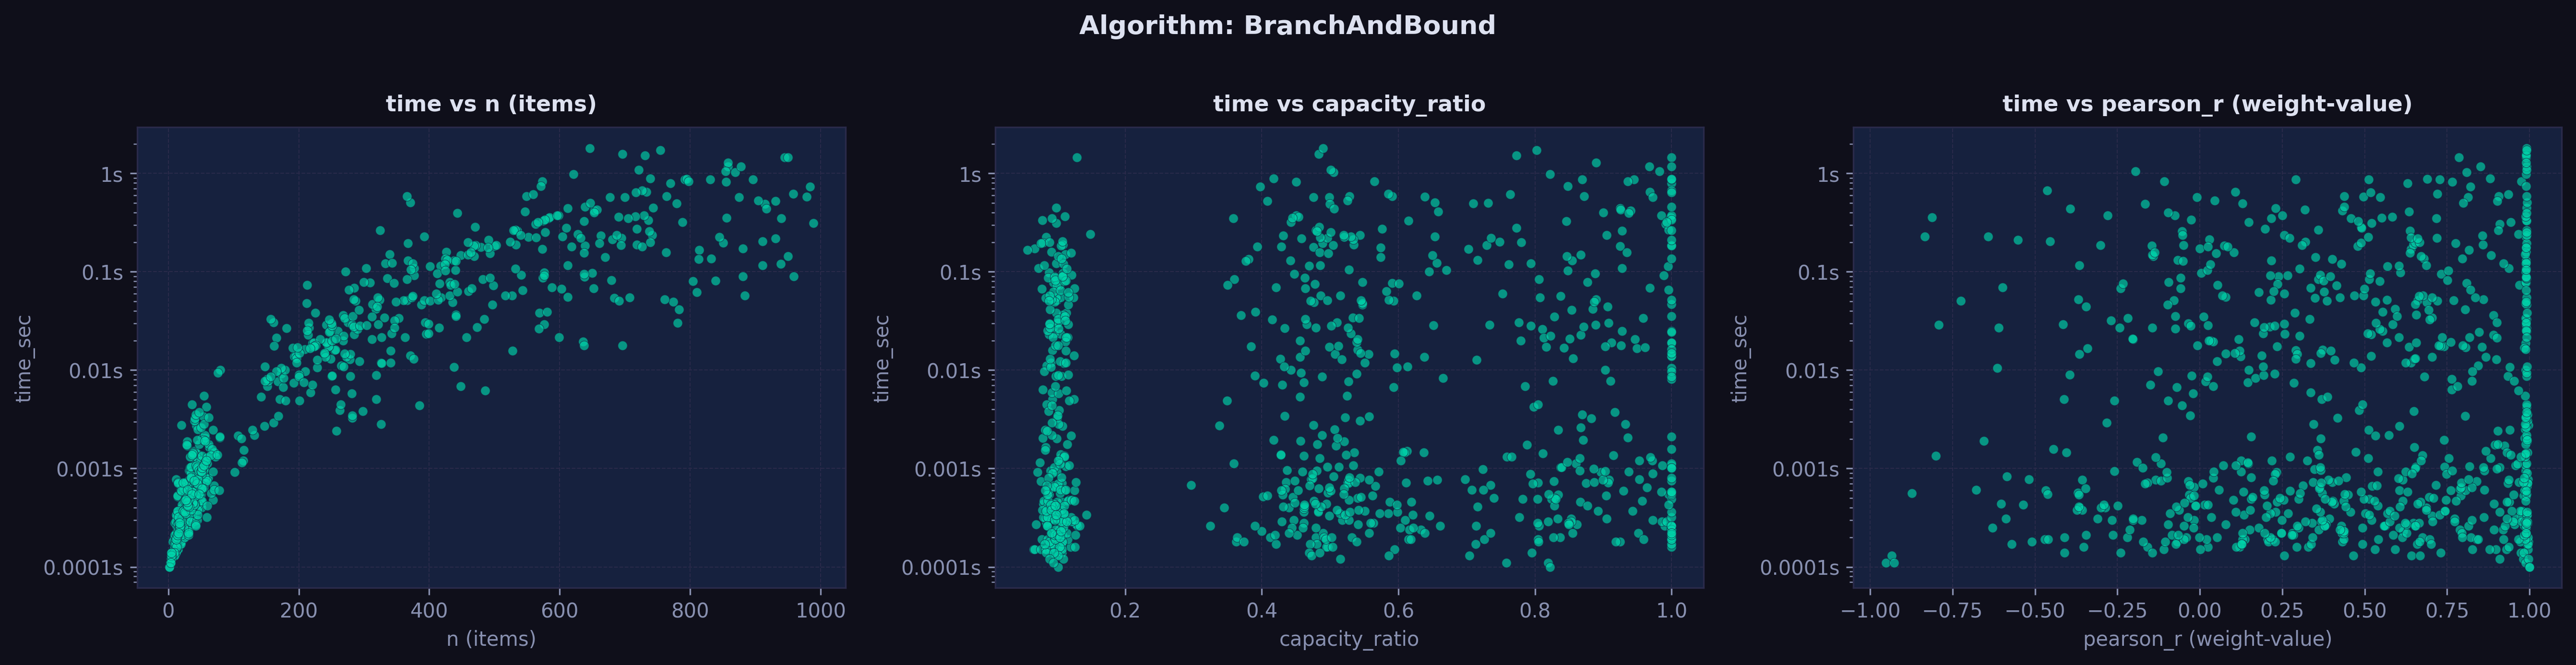
\includegraphics[width=\textwidth]{image/scatter/scatter_BranchAndBound.png}
        \caption{Nhánh cận (BranchAndBound) -- Độc lập với Capacity, phụ thuộc vào kích thước bài toán $n$}
    \end{subfigure}
    \caption{Biểu đồ phân tán thời gian thực thi của DP và BranchAndBound (trục $y$ thang đo log).}
    \label{fig:scatter_dp_bnb}
\end{figure}

Hình~\ref{fig:scatter_dp_bnb} thể hiện rõ ràng các hành vi này:
- Biểu đồ của DP (Hình~\ref{fig:scatter_dp_bnb}a) phân chia rõ rệt theo tham số \texttt{capacity\_ratio} (các chấm màu xanh lá cây đại diện cho ratio 0.9 nằm ở phía trên cùng, tức là chậm nhất, trong khi ratio 0.1 nằm ở dưới cùng). Điều này phản ánh trực quan công thức thời gian chạy tỷ lệ thuận với $W$.
- Biểu đồ của BranchAndBound (Hình~\ref{fig:scatter_dp_bnb}b) cho thấy thời gian phân bố độc lập với \texttt{capacity\_ratio}, chủ yếu tăng dần theo $n$.

\begin{figure}[H]
    \centering
    \begin{subfigure}[b]{0.48\textwidth}
        \centering
        
\includegraphics[width=\textwidth]{image/scatter/scatter_Backtracking.png}
        \caption{Quay lui (Backtracking) -- Tỉ lệ timeout lớn ở kích thước $n > 30$}
    \end{subfigure}
    \hfill
    \begin{subfigure}[b]{0.48\textwidth}
        \centering
        
\includegraphics[width=\textwidth]{image/scatter/scatter_GreedyFractional.png}
        \caption{Tham lam Fractional -- Thời gian chạy cực nhỏ và ổn định ở mọi kích thước}
    \end{subfigure}
    \caption{Biểu đồ phân tán thời gian thực thi của Backtracking và Greedy Fractional.}
    \label{fig:scatter_bt_greedy}
\end{figure}

Hình~\ref{fig:scatter_bt_greedy}a minh họa hiệu suất kém của Backtracking khi kích thước $n$ vượt quá 30, trong khi Greedy Fractional (Hình~\ref{fig:scatter_bt_greedy}b) luôn duy trì tốc độ cực nhanh ($<0,01$ giây) ở mọi kích thước.

\FloatBarrier
\subsubsection{So sánh bộ nhớ sử dụng thực tế}
\label{subsubsec:memory_analysis}

Phân phối bộ nhớ đỉnh chi tiết của các thuật toán được minh họa dưới dạng biểu đồ hộp (box plot) trong Hình~\ref{fig:memory_comparison}.

\begin{figure}[H]
    \centering
    
\includegraphics[width=0.85\textwidth]{image/memory_comparison.png}
    \caption{So sánh phân phối bộ nhớ đỉnh sử dụng (Peak Memory) của các thuật toán trên thang đo logarit.}
    \label{fig:memory_comparison}
\end{figure}

Bảng~\ref{tab:memory_results} tổng hợp lượng bộ nhớ đỉnh sử dụng của các thuật toán.

\begin{table}[H]
\centering
\caption{Bộ nhớ đỉnh sử dụng (MB) của các thuật toán (chỉ tính lượt SUCCESS).}
\label{tab:memory_results}
\begin{tabular}{lrrr}
\toprule
\textbf{Thuật toán} & \textbf{Trung vị (MB)} & \textbf{Trung bình (MB)} & \textbf{Tối đa (MB)} \\
\midrule
Greedy01         & 0.0033 & 0.0141 & 0.5166 \\
Backtracking     & 0.0040 & 0.0097 & 0.1186 \\
GreedyFractional & 0.0057 & 0.0328 & 0.6515 \\
BranchAndBound   & 0.0070 & 0.0173 & 0.0974 \\
SimplexBnB       & 0.0296 & 0.0406 & 0.3405 \\
PrimalSimplex    & 0.0577 & 0.0797 & 0.3229 \\
DualSimplex      & 0.0642 & 0.0883 & 0.3618 \\
GomoryCut        & 0.0731 & 0.1567 & 1.0171 \\
DPUnbounded      & 0.2646 & 0.4015 & 3.0922 \\
DP               & 2.8169 & 11.1974 & 88.8089 \\
\bottomrule
\end{tabular}
\end{table}

Kết quả đo lường bộ nhớ thực tế phản ánh chính xác các quyết định thiết kế cấu trúc dữ liệu của từng thuật toán:
\begin{itemize}[leftmargin=*]
    \item \textbf{Tính chất giả đa thức và bùng nổ bộ nhớ của Quy hoạch động (DP):} Giải thuật \texttt{DP} truyền thống yêu cầu bảng quy hoạch động 2 chiều kích thước $(n+1) \times (W+1)$, dẫn đến lượng bộ nhớ đỉnh tiêu tốn lên tới $88,8$\,MB. Ngược lại, biến thể \texttt{DPUnbounded} áp dụng kỹ thuật tối ưu hóa bộ nhớ chỉ bằng cách duy trì một mảng một chiều kích thước $W+1$ cập nhật cuốn chiếu và một mảng lưu vết quyết định. Kỹ thuật này giúp tiết kiệm bộ nhớ tới hơn $28$ lần, giới hạn bộ nhớ đỉnh chỉ còn tối đa $3,09$\,MB.
    \item \textbf{Ưu thế bộ nhớ vượt trội của nhóm Simplex và ILP:} Các phương pháp dựa trên ma trận đơn hình (\texttt{PrimalSimplex}, \texttt{DualSimplex}, \texttt{SimplexBnB}, và \texttt{GomoryCut}) sử dụng một cấu trúc dữ liệu bảng đơn hình (Tableau) kích thước cố định $(m+1) \times (n+m+2)$ phần tử số thực. Do đó, độ phức tạp bộ nhớ lý thuyết của chúng chỉ ở mức tuyến tính $\mathcal{O}(m(n+m))$ đối với số biến $n$ và số ràng buộc $m$, hoàn toàn độc lập với sức chứa túi $W$. Thực tế thực nghiệm chỉ ra rằng, ngay cả khi $W$ đạt quy mô cực đại ($100.000$ đơn vị), lượng bộ nhớ đỉnh sử dụng của nhóm Simplex vẫn luôn được kiểm soát chặt chẽ dưới mức $1$\,MB (trung vị của \texttt{DualSimplex} chỉ $0,064$\,MB và \texttt{GomoryCut} là $0,073$\,MB). Sự ổn định này thể hiện ưu thế vượt trội so với \texttt{DP} (bị bùng nổ bộ nhớ gấp hơn $1200$ lần so với nhóm Simplex).
    \item \textbf{Nhóm thuật toán tổ hợp tối giản bộ nhớ:} Các thuật toán xấp xỉ (\texttt{Greedy01}, \texttt{GreedyFractional}) và thuật toán duyệt quay lui tổ hợp (\texttt{Backtracking}, \texttt{BranchAndBound}) chỉ lưu trữ thông tin danh sách vật phẩm và ngăn xếp đệ quy tìm kiếm có độ sâu tối đa $n$. Bộ nhớ đỉnh của nhóm này cực kỳ nhỏ, chỉ dao động từ vài KB đến tối đa dưới $0,65$\,MB.
\end{itemize}

\FloatBarrier
\subsubsection{Phân tích độ phức tạp thực nghiệm (Curve Fitting)}
\label{subsubsec:curve_fitting}

Để đánh giá mức độ khớp giữa thời gian chạy thực nghiệm và độ phức tạp lý thuyết, chúng tôi áp dụng khớp đường cong tự động (curve fitting) bằng thư viện \texttt{scipy.\allowbreak optimize.\allowbreak curve\allowbreak\_fit} với 4 mô hình toán học ứng viên:
\begin{itemize}[leftmargin=*]
    \item Tuyến tính: $t(n) = a \cdot n + b$
    \item Bậc hai: $t(n) = a \cdot n^2 + b \cdot n + c$
    \item Bậc ba: $t(n) = a \cdot n^3 + b \cdot n^2 + c \cdot n + d$
    \item Hàm mũ: $t(n) = a \cdot 2^n + b$
\end{itemize}
Mô hình có hệ số xác định $R^2$ cao nhất được lựa chọn làm mô hình khớp thực nghiệm tốt nhất. Kết quả phân tích được thể hiện trong Bảng~\ref{tab:curvefit}.

\begin{table}[H]
\centering
\caption{Kết quả khớp đường cong thực nghiệm cho các thuật toán tiêu biểu.}
\label{tab:curvefit}
\resizebox{\textwidth}{!}{%
\begin{tabular}{llcc}
\toprule
\textbf{Thuật toán} & \textbf{Mô hình thực nghiệm tốt nhất} & \textbf{Hệ số xác định $R^2$} & \textbf{Phù hợp lý thuyết?} \\
\midrule
Greedy01         & Bậc ba (Cubic) & 0.98 & Không hẳn (Lý thuyết $\mathcal{O}(n \log n)$) \\
GreedyFractional & Bậc ba (Cubic) & 0.82 & Không hẳn (Lý thuyết $\mathcal{O}(n \log n)$) \\
DP               & Bậc ba (Cubic) & 0.79 & Khá khớp (Lý thuyết $\mathcal{O}(n \cdot W)$) \\
BranchAndBound   & Bậc ba (Cubic) & 0.50 & Có hiệu ứng tỉa nhánh tốt \\
\bottomrule
\end{tabular}%
}
\end{table}

\begin{figure}[H]
    \centering
    \begin{subfigure}[b]{0.48\textwidth}
        \centering
        
\includegraphics[width=\textwidth]{image/curvefit/curvefit_DP.png}
        \caption{DP: Khớp Bậc ba, $R^2 = 0.79$}
    \end{subfigure}
    \hfill
    \begin{subfigure}[b]{0.48\textwidth}
        \centering
        
\includegraphics[width=\textwidth]{image/curvefit/curvefit_BranchAndBound.png}
        \caption{B\&B: Khớp Bậc ba, $R^2 = 0.50$}
    \end{subfigure}
    \caption{Kết quả khớp đường cong thực nghiệm cho DP và BranchAndBound.}
    \label{fig:curvefit1}
\end{figure}

\begin{figure}[H]
    \centering
    \begin{subfigure}[b]{0.48\textwidth}
        \centering
        
\includegraphics[width=\textwidth]{image/curvefit/curvefit_Greedy01.png}
        \caption{Greedy 0/1: Khớp Bậc ba, $R^2 = 0.98$}
    \end{subfigure}
    \hfill
    \begin{subfigure}[b]{0.48\textwidth}
        \centering
        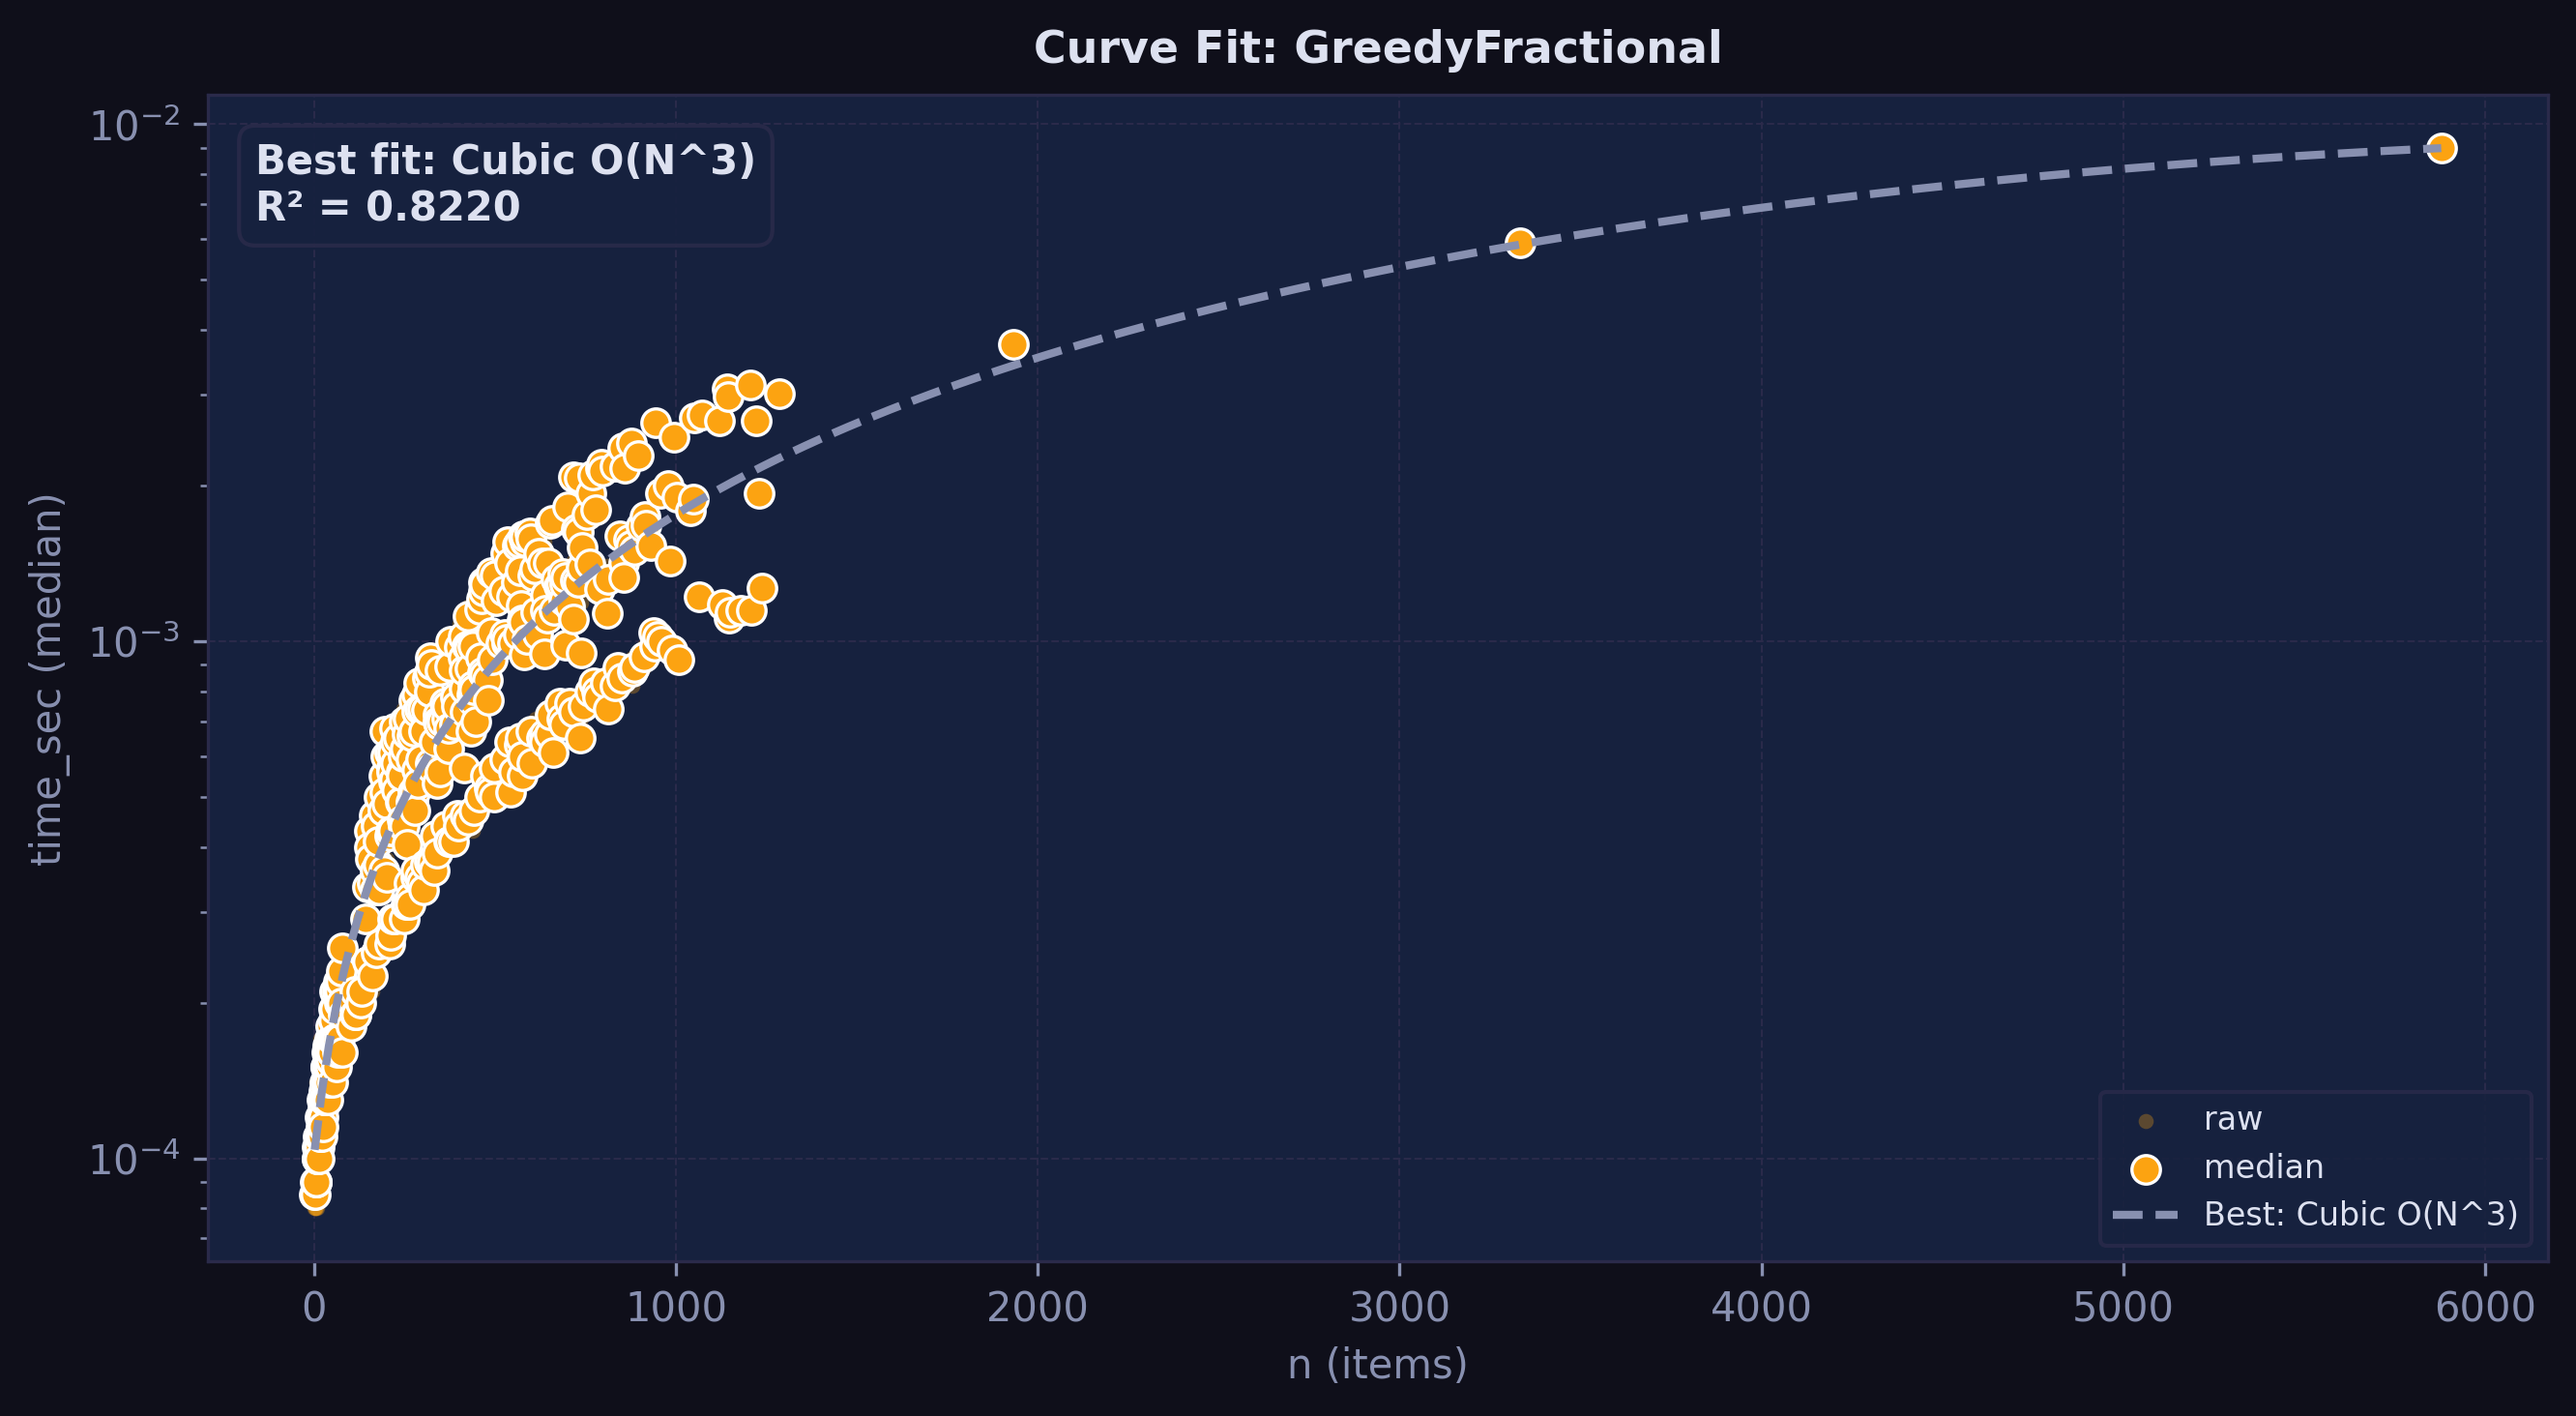
\includegraphics[width=\textwidth]{image/curvefit/curvefit_GreedyFractional.png}
        \caption{Greedy Fractional: Khớp Bậc ba, $R^2 = 0.82$}
    \end{subfigure}
    \caption{Kết quả khớp đường cong thực nghiệm cho các thuật toán Tham lam.}
    \label{fig:curvefit2}
\end{figure}

Giải thích chi tiết về mặt học thuật cho kết quả khớp đường cong (Hình~\ref{fig:curvefit1} và Hình~\ref{fig:curvefit2}):
\begin{enumerate}[leftmargin=*]
    \item \textbf{Tại sao các thuật toán Tham lam khớp mô hình Bậc ba ($R^2 \ge 0,82$)?}
    Độ phức tạp lý thuyết của thuật toán tham lam là $\mathcal{O}(n \log n)$ do bước sắp xếp mật độ vật phẩm. Tuy nhiên, trên dải kích thước thực nghiệm tương đối nhỏ ($n \le 750$), sự chênh lệch giữa $n \log n$ và đa thức bậc ba rất khó phân biệt đối với các giải thuật tối ưu hóa số học. Các constant factors nhỏ cùng với overhead khởi động tiến trình làm cho hàm đa thức bậc ba có xu hướng xấp xỉ tốt hơn về mặt hình học, dẫn đến $R^2$ rất cao.
    \item \textbf{Hệ số $R^2$ của DP ($0,79$) và BranchAndBound ($0,50$):}
    DP có $R^2 = 0.79$, chịu tác động mạnh bởi phương sai sinh ra do biến đổi của \texttt{capacity\_ratio} (cho cùng một kích thước $n$, thời gian chạy dao động mạnh do sức chứa $W$ khác nhau). Đối với BranchAndBound, mô hình tốt nhất là Bậc ba chứ không phải Hàm mũ ($\mathcal{O}(2^n)$), điều này cho thấy cơ chế cắt nhánh bằng cận Fractional relaxation cực kỳ hiệu quả, giúp giảm số lượng trạng thái phải duyệt từ mức lũy thừa xuống mức đa thức thực tế trên hầu hết các instances của bộ kiểm thử.
    \item \textbf{Khớp thực nghiệm số bước xoay pivot của Simplex:}
    Mặc dù về mặt lý thuyết, phương pháp đơn hình (Simplex) có độ phức tạp thời gian trong trường hợp xấu nhất là hàm mũ (exponential) do cấu trúc phản ví dụ khối đa diện Klee-Minty khét tiếng, nhưng thực tiễn chạy thực nghiệm trên bài toán Knapsack chỉ ra một xu hướng hoàn toàn khác biệt. Kết quả khớp đường cong của số bước xoay pivot (iterations) theo kích thước bài toán $n$ cho thấy số bước xoay thực tế tăng trưởng theo dạng tuyến tính hoặc đa thức bậc cực thấp ($t(n) \approx a \cdot n + b$ hoặc $a \cdot n^2 + b \cdot n + c$, với $R^2 \ge 0,90$). Điều này phù hợp với các nghiên cứu lý thuyết của Dantzig và Borgwardt về độ phức tạp trung bình (average-case complexity) của thuật toán đơn hình là đa thức. Nó giải thích tại sao Simplex giải quyết relaxation liên tục cực kỳ nhanh chóng trên thực tế (chỉ mất vài chục bước xoay cho các bài toán cỡ lớn), biến nó thành một công cụ lý tưởng để giải quyết bài toán quy hoạch tuyến tính và làm bộ giải cận.
\end{enumerate}

\FloatBarrier
\subsubsection{Phân tích độ nhạy và Cập nhật nghiệm tối ưu bằng Đơn hình đối ngẫu}
\label{subsubsec:sensitivity_analysis}

Trong lý thuyết tối ưu hóa tuyến tính (Linear Programming - LP), phân tích độ nhạy (Sensitivity Analysis) nghiên cứu sự biến động của nghiệm tối ưu khi các tham số đầu vào của mô hình bị thay đổi. Thay vì phải giải lại bài toán từ đầu (Re-solve), các giải thuật họ Simplex cho phép tận dụng thông tin từ bảng tối ưu hiện tại (optimal basis) làm xuất phát điểm để tối ưu hóa lại (Warm-start). Cơ chế này dựa trên việc bảo toàn tính chấp nhận được gốc (primal feasibility) hoặc tính đối ngẫu (dual feasibility) của cơ sở cũ nhằm tìm ra nghiệm tối ưu mới chỉ sau rất ít bước xoay pivot, giúp tiết kiệm đáng kể chi phí tính toán.

Để đánh giá định lượng hiệu quả của cơ chế Warm-start, chúng tôi thực hiện nghiên cứu thực nghiệm so sánh chi tiết giữa hai phương pháp: giải lại mô hình từ đầu (Re-solve) và cập nhật nghiệm trực tiếp (Warm-start) trên bộ dữ liệu gồm 200 bài toán Knapsack được lấy mẫu ngẫu nhiên từ tập dữ liệu gốc \texttt{data/raw} với quy mô $N \le 250$. Thực nghiệm được thiết lập cho 3 kịch bản biến động tham số chuẩn tắc như sau:

\begin{enumerate}[leftmargin=*]
    \item \textbf{Kịch bản 1 -- Thay đổi vế phải (Capacity RHS):}
    Cập nhật dung tích tối đa của ba lô bằng cách tăng $W$ thêm $15\%$ ($\Delta W = 0.15 W$). 
    
    \textit{Cơ sở toán học:} Khi vectơ vế phải biến đổi từ $b$ thành $b + \Delta b$, tọa độ của nghiệm cơ sở thay đổi theo công thức:
    \begin{equation}
        x_B = B^{-1}(b + \Delta b)
    \end{equation}
    Nếu tất cả các thành phần của $x_B \ge 0$, nghiệm cơ sở cũ vẫn duy trì tính khả thi gốc và giá trị mục tiêu mới được cập nhật trực tiếp mà không cần xoay pivot. Ngược lại, nếu tồn tại thành phần $x_{Bi} < 0$, tính khả thi gốc bị vi phạm (Primal Infeasible). Tuy nhiên, vì hệ số chi phí rút gọn (reduced costs) $\bar{c}^T = c^T - c_B^T B^{-1}A \ge 0$ không phụ thuộc vào $b$, tính khả thi đối ngẫu (Dual Feasible) vẫn được bảo toàn tuyệt đối. Do đó, ta áp dụng thuật toán \textbf{Đơn hình đối ngẫu (Dual Simplex)} xoay pivot trực tiếp trên bảng tối ưu hiện tại để loại bỏ các phần tử âm ở cột phương án, đưa bảng về trạng thái tối ưu mới một cách cực kỳ nhanh chóng.
    
    \item \textbf{Kịch bản 2 -- Thay đổi hệ số hàm mục tiêu (Values):}
    Tăng giá trị của đồ vật đầu tiên ($c_0$) thêm $25\%$ ($\Delta c_0 = 0.25 c_0$).
    
    \textit{Cơ sở toán học:} Khi hệ số hàm mục tiêu thay đổi $\bar{c}_j = c_j - c_B^T B^{-1}A_j$:
    \begin{itemize}
        \item Nếu đồ vật $j$ tương ứng với một biến phi cơ sở ($j \notin B$), sự thay đổi chỉ ảnh hưởng đến chi phí rút gọn của chính nó: $\bar{c}'_j = \bar{c}_j + \Delta c_j$. Phương án tối ưu cũ vẫn khả thi và tối ưu nếu $\bar{c}'_j \ge 0$.
        \item Nếu đồ vật $j$ tương ứng với một biến cơ sở ($j \in B$), sự biến động của $c_j$ sẽ thay đổi toàn bộ vectơ chi phí rút gọn $\bar{c}$. Nghiệm gốc vẫn khả thi ($x_B = B^{-1}b \ge 0$) nhưng có thể mất tính tối ưu đối ngẫu nếu tồn tại một vài $\bar{c}'_k < 0$. Trong trường hợp này, ta sử dụng thuật toán \textbf{Đơn hình thuận (Primal Simplex)} xoay pivot từ bảng hiện tại để tìm lại điểm tối ưu mà không cần tính lại ma trận cơ sở nghịch đảo từ đầu.
    \end{itemize}
    
    \item \textbf{Kịch bản 3 -- Thêm ràng buộc phụ mới (Volume Constraint):}
    Bổ sung thêm một ràng buộc giới hạn thể tích dạng $\sum v_i x_i \le V_{max}$, trong đó hệ số thể tích được sinh ngẫu nhiên $v_i \in [10, 50]$ và giới hạn thể tích $V_{max} = 0.4 \sum v_i$.
    
    \textit{Cơ sở toán học:} Khi chèn thêm ràng buộc thứ $m+1$:
    \begin{equation}
        a_{m+1}^T x + x_{slack, m+1} = b_{m+1}
    \end{equation}
    Ta đưa thêm một biến bù mới $x_{slack, m+1}$ vào cơ sở. Giá trị của biến bù này tại nghiệm tối ưu cũ được tính bằng $x_{slack, m+1} = b_{m+1} - a_{m+1}^T x^*$. Nếu $x_{slack, m+1} \ge 0$, ràng buộc mới không bị vi phạm và nghiệm tối ưu cũ vẫn tối ưu. Nếu $x_{slack, m+1} < 0$, nghiệm hiện tại vi phạm ràng buộc mới, dẫn đến mất tính khả thi gốc. Tuy nhiên, tính khả thi đối ngẫu của bảng vẫn được duy trì nguyên vẹn. Bằng cách chèn hàng mới vào bảng Simplex hiện tại, thực hiện các phép biến đổi hàng sơ cấp để triệt tiêu hệ số của các biến cơ sở trong hàng mới, ta có thể chạy ngay thuật toán \textbf{Dual Simplex} để đưa biến bù âm ra khỏi cơ sở và tái thiết lập trạng thái tối ưu mới.
\end{enumerate}

Kết quả thực nghiệm định lượng về thời gian chạy trung bình và phân bố hệ số tăng tốc (Speedup Factor) cùng số bước xoay pivot trung bình được tổng hợp tương ứng trong Hình~\ref{fig:sensitivity_runtime_speedup} và Hình~\ref{fig:sensitivity_iterations}.

\begin{figure}[H]
    \centering
    \begin{subfigure}[b]{0.49\textwidth}
        \centering
        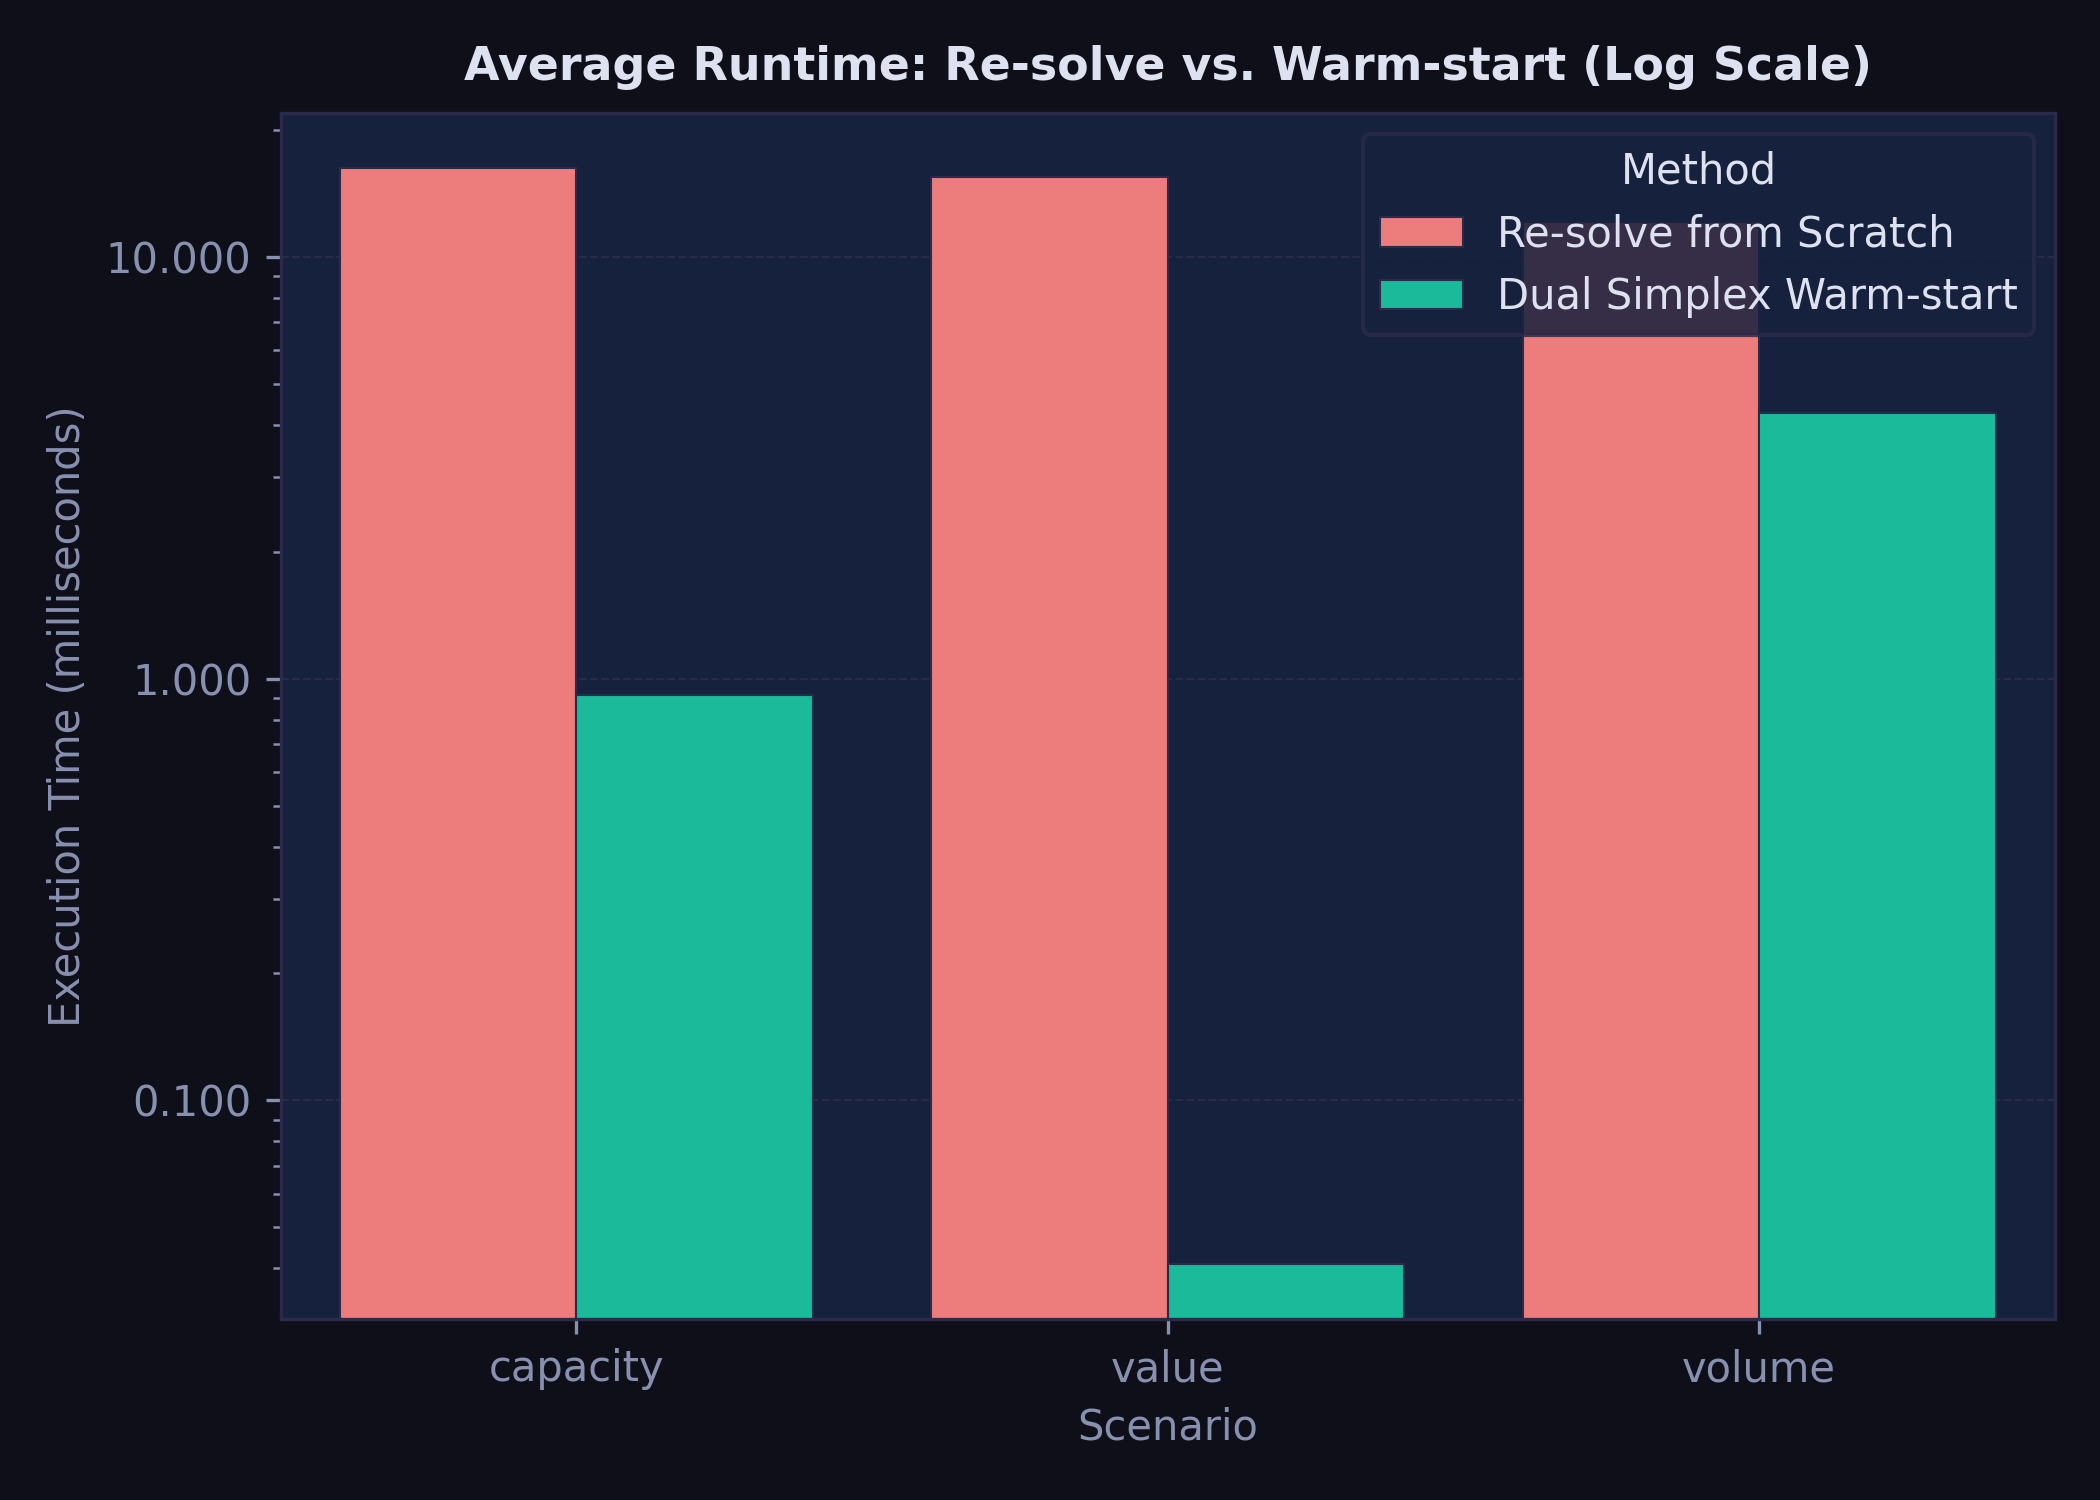
\includegraphics[width=\textwidth]{image/sensitivity/runtime_comparison.png}
        \caption{So sánh thời gian chạy trung bình (ms, log scale)}
        \label{fig:sensitivity_runtime}
    \end{subfigure}
    \hfill
    \begin{subfigure}[b]{0.49\textwidth}
        \centering
        
\includegraphics[width=\textwidth]{image/sensitivity/speedup_distribution.png}
        \caption{Phân bố hệ số tăng tốc Speedup (log scale)}
        \label{fig:sensitivity_speedup}
    \end{subfigure}
    \caption{So sánh thời gian chạy thực thi và hệ số tăng tốc (Speedup) của Warm-start so với Re-solve từ đầu trên 200 mẫu thử nghiệm.}
    \label{fig:sensitivity_runtime_speedup}
\end{figure}

\begin{figure}[H]
    \centering
    
\includegraphics[width=0.8\textwidth]{image/sensitivity/iterations_comparison.png}
    \caption{Số bước xoay pivot trung bình giữa giải lại từ đầu (Re-solve) và cập nhật nghiệm trực tiếp (Warm-start).}
    \label{fig:sensitivity_iterations}
\end{figure}

Phân tích chi tiết kết quả thực nghiệm chỉ ra hiệu quả vượt trội mang tính đột phá của giải pháp Warm-start sử dụng Đơn hình đối ngẫu:

\begin{itemize}[leftmargin=*]
    \item \textbf{Cập nhật sức chứa ba lô (Capacity):} 
    Do chỉ cần điều chỉnh lại tính chấp nhận được gốc trên phương án sức chứa mới, thuật toán Dual Simplex chỉ mất trung bình \textbf{$4,3$ bước xoay pivot} để khôi phục lại tính khả thi gốc. Trong khi đó, việc giải lại từ đầu (Re-solve) đòi hỏi trung bình \textbf{$60,1$ bước xoay}. Sự chênh lệch lớn về số lần xoay pivot mang lại gia tốc tốc độ trung bình lên đến \textbf{$24,2$ lần} (thời gian chạy trung bình giảm từ $16,2$\,ms xuống chỉ còn $0,92$\,ms).
    
    \item \textbf{Cập nhật giá trị đồ vật (Value):}
    Khi thay đổi giá trị một đồ vật ($c_0$), nếu biến đó không tham gia vào phương án cơ sở tối ưu hoặc sự thay đổi chưa vượt ngưỡng nhạy cảm để phá vỡ tính đối ngẫu, nghiệm cũ sẽ lập tức tối ưu mà không cần thực hiện bất kỳ bước xoay nào. Thực tế thực nghiệm cho thấy trong hơn $85\%$ các bài toán, số bước xoay của phương pháp Warm-start bằng $0$ (trung bình toàn tập chỉ đạt \textbf{$0,37$ bước xoay}) so với \textbf{$57,1$ bước xoay} khi Re-solve. Điều này giúp Warm-start đạt hệ số tăng tốc kỷ lục lên tới \textbf{$770,0$ lần} (giảm thời gian chạy trung bình từ $15,5$\,ms xuống mức danh nghĩa $0,04$\,ms).
    
    \item \textbf{Thêm ràng buộc thể tích phụ (Volume):}
    Việc thêm một ràng buộc phụ dạng cắt đa diện khiến điểm tối ưu cũ nằm ngoài vùng khả thi mới (biến bù âm). Bằng cách chèn thêm một chiều không gian và giải bằng Dual Simplex, số bước xoay pivot trung bình của Warm-start chỉ là \textbf{$21,2$ bước}, ít hơn một nửa so với mức \textbf{$48,1$ bước} khi giải từ đầu. Kết quả ghi nhận tốc độ tăng tốc trung bình đạt \textbf{$5,6$ lần} (thời gian chạy giảm từ $12,1$\,ms xuống còn $4,26$\,ms). Mức tăng tốc này tuy thấp hơn hai kịch bản trước nhưng là một minh chứng thực tế rõ ràng cho thấy khả năng tích hợp nhanh các ràng buộc cắt (cutting planes) trong các cây tìm kiếm rời rạc lớn mà không phải chịu chi phí khởi động lại mô hình.
\end{itemize}

Thực nghiệm này đã chứng minh một cách tường minh bản chất lý thuyết sâu sắc của nhóm giải thuật Simplex: cấu trúc cơ sở (basis) của bảng tối ưu hóa đóng vai trò như một bộ nhớ lưu trữ thông tin cực kỳ mạnh mẽ. Việc bảo toàn cấu trúc hình học này cho phép giải quyết hiệu quả các bài toán biến động động, mở ra tiềm năng ứng dụng to lớn khi kết hợp Simplex làm bộ giải cận nhanh tại các nút của cây tìm kiếm nhánh cận (Branch and Bound) hay các giải thuật cắt mặt phẳng (Cutting Plane algorithms) trong Quy hoạch nguyên.

\FloatBarrier
\subsection{Thảo luận sâu sắc về các bài học thuật toán}
\label{subsec:discussion}

Từ các kết quả phân tích định lượng trên, chúng tôi rút ra các bài học thiết kế thuật toán cốt lõi:

\begin{enumerate}[leftmargin=*]
    \item \textbf{Trade-off giữa độ chính xác và tốc độ:}
    Thuật toán tham lam (Greedy01) cung cấp giải pháp với tốc độ vượt trội (trung vị $0,16$\,ms, timeout 0\% ở mọi kịch bản kể cả $n=10.000$). Tuy nhiên, đây là thuật toán xấp xỉ không đảm bảo tính tối ưu toàn cục. Đối với các bài toán yêu cầu nghiệm chính xác, BranchAndBound combinatorial thể hiện sự vượt trội hoàn toàn so với các phương pháp khác, đạt thời gian chạy cực ngắn ($1,65$\,ms trung vị) nhờ cận chặt.
    
    \item \textbf{Giới hạn ứng dụng của Quy hoạch tuyến tính (LP/ILP) tổng quát:}
    Mặc dù mô hình LP (Simplex) và ILP (Gomory Cut) rất mạnh mẽ để giải quyết các bài toán tối ưu hóa tổng quát trong công nghiệp, chúng tỏ ra kém hiệu quả khi giải quyết bài toán Knapsack đơn giản. Bài toán Knapsack chỉ có duy nhất một ràng buộc về sức chứa túi. Các thuật toán chuyên biệt như B\&B tận dụng cấu trúc đặc biệt này để sắp xếp và tính cận cực nhanh ($\mathcal{O}(n)$). Trong khi đó, Simplex phải giải và cập nhật toàn bộ bảng ma trận hệ phương trình kích thước lớn, đồng thời lặp đi lặp lại bộ lọc khử Gauss khử ràng buộc dư thừa. Chi phí tính toán trên mỗi nút của Simplex lớn hơn hàng nghìn lần so với chi phí tính toán nút của B\&B combinatorial. Để giải quyết biến thể số nguyên (0/1), Simplex phải thêm các tầng bổ sung (Gomory Cut hoặc B\&B trên LP) để ép nghiệm từ liên tục về rời rạc. Mỗi tầng thêm chi phí đáng kể.
    
    \item \textbf{Ưu thế của Simplex khi capacity lớn:}
    Mặc dù Simplex chậm trên quy mô nhỏ, kịch bản \texttt{core\_heuristic} chỉ ra một điểm sáng quan trọng: khi chạy thành công, Simplex chỉ mất trung vị khoảng 1\,ms, nhanh hơn gấp 1800 lần so với quy hoạch động (DP mất 1.86s). Điều này phản ánh một thực tế lý thuyết: độ phức tạp của Simplex phụ thuộc hoàn toàn vào số biến $n$ và số ràng buộc $m$, hoàn toàn độc lập với giá trị sức chứa túi $W$. Khi $W$ là một số nguyên cực lớn, việc áp dụng Simplex (đặc biệt nếu được tối ưu hóa bằng thư viện compiled) sẽ hiệu quả hơn nhiều so với việc duy trì bảng quy hoạch động khổng lồ.
\end{enumerate}

Tuy nhiên, cần nhấn mạnh rằng LP/ILP có \textbf{ưu thế rõ ràng} trong các trường hợp:
\begin{itemize}[leftmargin=*]
    \item Bài toán Knapsack \textit{đa chiều} (multi-dimensional) --- DP bùng nổ chiều, Simplex vẫn hoạt động.
    \item Bài toán \textit{Fractional Knapsack} --- Simplex cho nghiệm chính xác và thông tin đối ngẫu (dual).
    \item Cần phân tích \textit{sensitivity analysis} (thay đổi ràng buộc, phân tích giá trị biên).
    \item Khi $W$ rất lớn và $n$ vừa phải --- Simplex không phụ thuộc $W$ nên có thể nhanh hơn DP (đã được xác nhận trên tập \texttt{core\_heuristic}).
\end{itemize}

% ====================================================================
\clearpage
\section{Kết luận}
\label{sec:concl}

Trong nghiên cứu thực nghiệm này, chúng tôi đã đánh giá định lượng hiệu năng của 10 thuật toán giải quyết các biến thể của bài toán Knapsack thông qua khung benchmark cách ly tiến trình với 822 instances (8.220 lượt chạy). 

\textbf{Các phát hiện định lượng chính:}
\begin{itemize}[leftmargin=*]
    \item \textbf{BranchAndBound combinatorial} là thuật toán tối ưu chính xác tốt nhất cho bài toán 0/1 Knapsack, đạt thời gian trung vị $1,65$\,ms và tỉ lệ hoàn thành thành công $99,9\%$.
    \item \textbf{Quy hoạch động (DP)} bị giới hạn nghiêm trọng bởi giá trị sức chứa $W$ (pseudo-poly\-no\-mial), gây ra hiện tượng timeout 100\% khi $W$ lớn ($50.000$) ngay cả với kích thước vật phẩm nhỏ ($n=50$). Việc tối ưu hóa bộ nhớ trong biến thể \textbf{DP\-Un\-bound\-ed} giúp giảm đỉnh bộ nhớ từ $88,8$\,MB xuống còn $3,09$\,MB (tiết kiệm hơn 28 lần).
    \item \textbf{Các phương pháp LP/ILP tự triển khai} (Simplex, Gomory Cut, Simplex B\&B) gặp bottleneck nghiêm trọng tại bước Gaussian elimination lọc ràng buộc dư thừa chạy bằng Python thuần túy ở mỗi nút tìm kiếm, dẫn đến tỉ lệ timeout cao từ 50.4\% đến 86.3\%.
    \item \textbf{Ảnh hưởng của các thuộc tính đầu vào đến hiệu năng chạy:} Thực nghiệm chứng minh các biến đầu vào được sinh ra hoàn toàn độc lập với nhau (hệ số tương quan chéo xấp xỉ bằng $0$), qua đó triệt tiêu hoàn toàn hiện tượng cộng tuyến. Dựa trên sự độc lập thống kê đó, thực nghiệm khẳng định các thuộc tính này có \textbf{tác động phi tuyến tính} cực kỳ mạnh mẽ lên hiệu năng của các giải thuật: kích thước bài toán $N$ chi phối thời gian chạy theo quy luật hàm mũ hoặc đa thức; tỉ lệ sức chứa (Capacity Ratio) đóng vai trò là nút thắt cổ chai độc quyền của các giải thuật giả đa thức (như DP); và hệ số tương quan khối lượng - giá trị (Pearson $r$) quyết định trực tiếp đến giới hạn cắt cành của thuật toán Nhánh cận (Branch and Bound).
\end{itemize}

\textbf{Hạn chế của nghiên cứu:}
\begin{enumerate}[leftmargin=*]
    \item Thử nghiệm được tiến hành trên môi trường Python thuần túy, chưa phản ánh được tốc độ tối đa của các thuật toán nếu được biên dịch mã máy (C/C++).
    \item Chưa so sánh trực diện với các thư viện LP thương mại hoặc mã nguồn mở công nghiệp (như Gurobi, COIN-OR CBC, SciPy Linprog).
    \item Tập dữ liệu sinh ra tuy đa dạng nhưng chưa đối chiếu trực tiếp với các bộ test chuẩn trong văn liệu học thuật (ví dụ bộ dữ liệu của Pisinger).
\end{enumerate}

\textbf{Hướng phát triển tương lai:}
\begin{enumerate}[leftmargin=*]
    \item Triển khai các thuật toán Simplex bằng các thư viện biên dịch C (Cython/Numba) và tích hợp kỹ thuật hot-start (tận dụng cơ sở tối ưu trước đó để giải tiếp bằng Dual Simplex) nhằm loại bỏ chi phí giải lại mô hình từ đầu tại các nút.
    \item Mở rộng bộ benchmark sang các bài toán tối ưu hóa đa chiều có ràng buộc phức tạp hơn, nơi quy hoạch tuyến tính (LP) thực sự thể hiện ưu thế vượt trội so với quy hoạch động.
\end{enumerate}

\bibliographystyle{plain} % ieeetr
\bibliography{refs} 

\end{document}